% !TeX program = pdflatex
\RequirePackage{amsmath}
\documentclass[lineno,paper]{JFM-FLM_Au}

% Canonical manuscript; main.tex selects the yellow revision copy.
\usepackage{xcolor}
\usepackage[most]{tcolorbox}
\definecolor{revisionyellow}{rgb}{1,1,0.55}
\ifdefined\ShowRevisionMarkup
\newenvironment{revision}{\nolinenumbers\begin{tcolorbox}[breakable,colback=revisionyellow,colframe=revisionyellow,boxrule=0pt,arc=0pt,left=5pt,right=5pt,top=5pt,bottom=5pt,before skip=6pt,after skip=6pt]\captionsetup{width=\linewidth}}{\end{tcolorbox}\linenumbers}
\DeclareRobustCommand{\revisionheading}[1]{\colorbox{revisionyellow}{\strut #1}}
\newcommand{\revisionbox}[1]{\colorbox{revisionyellow}{#1}}
\else
\newenvironment{revision}{}{}
\DeclareRobustCommand{\revisionheading}[1]{#1}
\newcommand{\revisionbox}[1]{#1}
\fi
\newtheorem{lemma}{Lemma}
\newtheorem{proposition}{Proposition}
\newtheorem{remark}{Remark}
\newcommand{\Kn}{\mathit{Kn}}
\newcommand{\dd}{\mathrm{d}}
\newcommand{\cl}{\mathrm{cl}}
\newcommand{\DVM}{\mathrm{DVM}}
\newcommand{\PINN}{\mathrm{PINN}}
\newcommand{\tr}{\operatorname{tr}}
\newcommand{\dev}{\operatorname{dev}}

% JFM's custom appendix resets section counters after hyperref is loaded.
% Give PDF destinations distinct namespaces without changing printed numbers.
\renewcommand*{\theHsection}{\ifappendix appendix.\Alph{section}\else main.\arabic{section}\fi}
\renewcommand*{\theHsubsection}{\theHsection.\arabic{subsection}}
\renewcommand*{\theHsubsubsection}{\theHsubsection.\arabic{subsubsection}}
\renewcommand*{\theHequation}{\theHsection.\arabic{equation}}

\lefttitle{E. Roohi}
\righttitle{Closure-channel identifiability in kinetic shocks}

\title{Closure-channel identifiability and two-channel recovery in monatomic kinetic normal shocks}

\author{Ehsan Roohi\aff{1}}

\affiliation{\aff{1}Department of Mechanical and Industrial Engineering, University of Massachusetts Amherst, Amherst, MA 01003, USA}

\corresau{Ehsan Roohi, \email{eroohi@umass.edu}}

\begin{document}
\maketitle
\raggedbottom
\setlength{\abovedisplayskip}{7pt}
\setlength{\belowdisplayskip}{7pt}
\setlength{\abovedisplayshortskip}{4pt}
\setlength{\belowdisplayshortskip}{4pt}


\begin{abstract}
\begin{revision}
Residual agreement in a heat-flux equation does not uniquely identify the higher-order moments entering a monatomic normal shock. We formulate this limitation as an observation-map problem: the heat-flux budget determines the composite fourth-order channel $S=R^{\cl}_{xx}+\Delta/3$, rather than the tensorial closure moment $R^{\cl}_{xx}$ and scalar fourth-order excess $\Delta$ separately. The map has a one-dimensional null space. A complementary scalar-excess budget, evaluated consistently with the discrete velocity method (DVM), supplies the missing information. For Bhatnagar--Gross--Krook (BGK) reference shocks at Mach 2, 3 and 5, two-budget recovery reduces the active-zone tensorial-moment error from approximately $63$--$64\%$ to $2.54$--$4.43\%$. Exploratory moment evaluations at Mach 6, 8 and 12 retain a substantial scalar contribution. Sparse scalar measurements provide an information-reduction test whose accuracy depends on shock-core coverage. Shakhov, independently evolved finite-time ellipsoidal-statistical BGK (ES-BGK) shocks at Mach 2 and 3, ellipsoidal-statistical Fokker--Planck (ES-FP) source diagnostics, and direct simulation Monte Carlo (DSMC) diagnostics distinguish the collision-independent observation channel from collision-dependent scalar production. Completed Mach-5 DVM sensitivity tests give differences below $0.53\%$ for the six tested fields. A separate DSMC sampler comparison at 960 particles per cell gives moment-profile differences of $0.73$--$0.93\%$, comparable to sampling uncertainty; the collision-source difference is $1.41\%$. The central result is an identifiability principle: recovering tensorial and scalar fourth-order closure information requires an independent scalar complement to the heat-flux observation channel.
\end{revision}
\end{abstract}

\section{Introduction}
\label{sec:introduction}

\begin{revision}
A rarefied shock is a velocity-space object.  Its density, velocity and temperature are low-order projections of the molecular distribution, while closure variables in Grad-type and regularised moment systems are higher-order, sign-changing and tail-weighted projections.  The latter are especially sensitive to high-peculiar-speed tails, where sign-changing cancellations are almost invisible to density and velocity but dominate fourth-order transport.  This distinction is central in kinetic gas theory \citep{Cercignani1988,Sone2007,Bird1994} and in reduced moment models descended from Grad's expansion \citep{Grad1949,Levermore1996,Struchtrup2005,Torrilhon2016}.  In the regularised 13- and 26-moment hierarchies, higher moments are not optional diagnostics: the stress equation transports third-order information, and the heat-flux equation transports fourth-order information \citep{StruchtrupTorrilhon2003,TorrilhonStruchtrup2004,StruchtrupTorrilhon2007PRL,GuEmerson2009R26}.  In the regularised 26-moment (R26) system, the third-order tensor $m_{ijk}$, the fourth-order tensor $R^{\cl}_{ij}$ and the scalar fourth-order excess $\Delta$ are promoted to closure-level variables.  A kinetic solver or reduced model that reproduces the visible shock profile but misses these variables has not recovered the closure information needed by the moment hierarchy.
\end{revision}

\begin{revision}
Normal shocks are a particularly stringent test of this issue.  They have long served as kinetic benchmarks for the Boltzmann equation, direct simulation Monte Carlo (DSMC), moment closures and model kinetic equations because the shock layer concentrates transport, production and tail populations into a narrow spatial region \citep{MottSmith1951Shock,Alsmeyer1976Shock,IvanovGimelshein1998Hypersonic}.  Recent comparisons of Bhatnagar--Gross--Krook (BGK), Shakhov, ellipsoidal-statistical BGK (ES-BGK) and Fokker--Planck variants confirm that models with similar lower-order transport can differ substantially in higher-order moments in shock waves \citep{FeiLiuLiuZhang2020ShockBenchmark}.  This makes the normal shock an appropriate base problem for asking not only whether a solver reproduces low-order fields, but also which closure content its residuals actually identify.
\end{revision}

\begin{revision}
The issue considered in this paper is increasingly relevant because residual-based and physics-informed neural solvers are now used for kinetic equations \citep{Raissi2019PINN,Karniadakis2021PINNs,LouMengKarniadakis2021PINNBGK,Oh2025SPINNBGK}.  Such solvers are commonly validated using low-order profiles or small residuals in selected moment equations.  That practice is potentially misleading in rarefied flows: a residual can be exactly satisfied while observing only a projected part of the nonequilibrium distribution.  A companion neural-shock study \citep{Roohi2026NeuralShock} showed this failure mode empirically: a residual-consistent BGK shock solver could recover the macroscopic profiles and several lower nonequilibrium moments while leaving the tensorial fourth-order closure moment poorly determined.  We examine the information content of the kinetic budgets independently of the neural architecture.  Specifically, we ask which fourth-order closure content is observable from the heat-flux budget of a normal shock.  The answer is structural: the heat-flux budget selects a combined channel, while recovery of the tensorial closure moment itself requires one additional scalar fourth-order channel.
\end{revision}

\begin{revision}
We separate two questions: which fourth-order projection appears in the heat-flux flux, and how collisions produce or relax its scalar-excess component. Deterministic discrete-velocity-method (DVM) references allow us to evaluate budgets without particle-sampling noise. BGK supplies the reference two-budget reconstruction; Shakhov tests the effect of correcting heat-flux relaxation; ES-BGK and ellipsoidal-statistical Fokker--Planck (ES-FP) test scalar-source corrections due to anisotropic targets and diffusion. A separate DSMC calculation measures scalar production directly from accepted binary collisions. The observation channel is kinematic, whereas its complementary scalar-source law depends on the collision operator.
\end{revision}

\begin{revision}
Data-driven moment reduction also addresses the closure problem directly. \citet{Han2019MomentClosure} learn generalized moments and their dynamics from kinetic solutions, while \citet{Huang2023HyperbolicClosure} enforce global hyperbolicity in a learned radiative-transfer closure. These approaches concern reduced dynamics and structural constraints. Our question is complementary: given the specific heat-flux observation map of a normal shock, which fourth-order components can its residual identify? The rank test below addresses that map, rather than establishing a limitation of every data-driven closure or replacing their realizability and stability constraints.
\end{revision}

\begin{revision}
The gap addressed here is between validation of an observable and identification of its underlying closure variables. Agreement in a projected budget tests that projection; it does not determine components in the observation map's null space. Consequently, comparisons of shock profiles and collision-model source laws, while necessary, do not alone answer the identifiability question posed here. We separate three tasks: identifying the observable channel, supplying independent scalar information, and testing the numerical reliability of the resulting reconstruction. This distinction makes the contribution complementary to established moment hierarchies and kinetic shock benchmarks rather than a replacement for them.
\end{revision}

\begin{revision}
We first derive the heat-flux observation operator and its null space, then construct the complementary scalar-excess budget. The numerical tests examine budget recovery at Mach 2, 3 and 5, direct fourth-order moments at Mach 6, 8 and 12, sparse and noisy scalar measurements, and collision-model source diagnostics. A standalone DSMC calculation accumulates changes in $|\boldsymbol c|^4$ over accepted collisions. The contribution is the identification and reconstruction of the tensorial--scalar split within established moment budgets; it introduces neither a new R26 balance law nor a neural solver.
\end{revision}

\section{Kinetic shocks, R26 moments and DVM references}
\label{sec:reference}
\begin{revision}
We use $Pr=\mu c_p/\kappa$, where $\mu$ is dynamic viscosity,
$\kappa$ thermal conductivity and $c_p=5R/2$ the monatomic specific
heat at constant pressure. The specific gas constant $R$ is one in
computational units; $R^{\cl}_{ij}$ instead denotes a fourth-order
closure moment. The upstream Mach number is
$M_1=u_1/\sqrt{\gamma RT_1}$, with $\gamma=5/3$.
Subscripts 1 and 2 denote upstream and downstream reservoir states,
respectively, and $p=\rho RT$ is the scalar pressure.
The third-order tensor $m_{ijk}$ is the symmetric trace-free third
central moment of the molecular distribution.
\end{revision}

\begin{revision}
The calculations comprise several distinct solver campaigns. The Prandtl number is selected by the collision model and its parameters, not by the Mach number. In particular, the BGK budget references at $M_1=2,3,5$ and the BGK moment extension at $M_1=6,8,12$ have $Pr=1$. The separate transport-matched Shakhov DVM profiles at $M_1=2,3,4,5$ have $Pr=2/3$, as do the corrected-Shakhov R26 profiles reported at $M_1=2,3$. The separate published-profile Mach-8 Shakhov benchmark also uses $Pr=2/3$, but has a different viscosity law. Table~\ref{tab:solver_campaigns} identifies these campaigns before their results are compared. The monatomic value $2/3$ corrects heat-flux relaxation relative to viscous relaxation; it does not make Shakhov, R26 and DSMC collision production identical.
\end{revision}

\begin{table}
\centering
\revisionbox{\begin{minipage}{0.90\linewidth}\captionsetup{width=\linewidth}\caption{Collision model, transport parameters and numerical scope of the separate campaigns. BGK, Shakhov and the separate Mach-2/3 ES-BGK rows are evolved kinetic calculations; ES source-diagnostic rows are evaluations on BGK distributions. The DSMC Prandtl number is a transport consequence of the collision model, rather than an input relaxation-target parameter. Finite-time snapshots and completed prescribed step counts do not certify stationarity.}
\label{tab:solver_campaigns}\end{minipage}}\par
\small\raggedright\setlength{\tabcolsep}{3pt}
\begin{tabular}{p{0.25\linewidth}p{0.13\linewidth}p{0.09\linewidth}p{0.22\linewidth}p{0.22\linewidth}}
\toprule
Campaign & $M_1$ & $Pr$ & Relaxation/transport & Scope\\
\midrule
BGK budget references & $2,3,5$ & $1$ & Constant $\tau=1$, $\mu=p\tau$ & Full 3V DVM; two-budget recovery\\
BGK sensitivity / high-Mach extension & $5$ / $6,8,12$ & $1$ & Constant $\tau=1$ & Prescribed-step upwind DVM; exploratory high-Mach moments\\
Shakhov cross-method DVM & $2,3,4,5$ & $2/3$ & $\mu=T$, $\tau=1/\rho$ & Reduced-velocity, finite-time profiles\\
Corrected Shakhov R26 & $2,3$ & $2/3$ & $\mu=T$, $\tau=1/\rho$ & Steady residual solve with independent finite-tolerance qualification\\
Shakhov published-profile benchmark & $8$ & $2/3$ & $\mu=\mu_{\rm ref}T^{0.81}$ & Reduced-velocity upwind DVM; positivity/stationarity limitations\\
ES-BGK / ES-FP source diagnostics & $2,3,5$ & $2/3$ & $\alpha_{\rm ES}=-1/2$, $\beta=-5/4$ & Source post-processing on BGK fields\\
Independent ES-BGK DVM & $2,3$ & $2/3$ & $\mu=T$, $\tau_{\rm ES}=3/(2\rho)$ & Evolved finite-time shocks; appendix~\ref{app:esbgk_evolved}\\
DSMC collision-production ensemble & $3$ & Model-derived & Hard-sphere collisions & Eight-seed original/corrected sampler comparisons\\
DSMC high-particle profiles & $2,3,4,5$ & Model-derived & variable hard sphere (VHS) $\omega=1$, isotropic scattering & One seed per Mach; finite-time sampling\\
\bottomrule
\end{tabular}\par
\end{table}

\begin{revision}
We begin with the steady one-dimensional BGK model \citep{Bhatnagar1954},
\begin{equation}
  v_x\partial_x f = \frac{1}{\Kn}\{M[f]-f\},
  \label{eq:bgk}
\end{equation}
Here $\Kn=\tau v_0/L_0$ is the dimensionless relaxation coefficient. We choose $v_0=\sqrt{RT_1}$ and, for the BGK budget profiles, $L_0=\lambda_{\rm rel,1}=v_0\tau_1$, the upstream relaxation length. With constant $\tau=\tau_1$, this gives $\Kn=1$ and the collision update $\exp(-\Delta t)$ in computational units. Here $\Kn=1$ follows from choosing the upstream relaxation
length as the reference length; it does not mean that the
mean free path equals the full computational-domain length.
The factor $\exp(-\Delta t)$ expresses relaxation over a
time step measured in units of $\tau_1$. This choice of units
does not itself determine numerical accuracy, which must
be assessed through spatial, velocity-space and time-step
resolution. The label $x/\lambda_1$ on these BGK plots denotes $x/\lambda_{\rm rel,1}$; it does not identify this length with a hard-sphere mean free path. A domain-scaled coordinate, $\texttt{x\_scaled}=\texttt{x\_mfp}/(2H)$, and coefficient $\texttt{kn\_eff}=1/(2H)$ are also stored by the driver, where $H$ is the half-domain length in relaxation units. The reported BGK budgets use the unscaled relaxation-length coordinate and unit source rate. The Shakhov and DSMC campaigns specify their distinct transport and spatial conventions below.

Here $f(x,\boldsymbol v)$ is the distribution and $M[f]$ is the local Maxwellian with the same density $\rho$, streamwise velocity $u_x$ and temperature $T$ as $f$.  The peculiar velocity is $\boldsymbol c=\boldsymbol v-u_x\boldsymbol e_x$.  The heat flux and normal stress are
\begin{equation}
  q_x = \frac{1}{2}\int |\boldsymbol c|^2 c_x f\,\dd\boldsymbol v,
  \qquad
  \sigma_{xx}=\int \left(c_x^2-\frac{|\boldsymbol c|^2}{3}\right)f\,\dd\boldsymbol v .
  \label{eq:q_sigma}
\end{equation}

The coordinate $x$ is normal to the shock, $\boldsymbol v$ is the
molecular velocity and $\boldsymbol e_x$ the streamwise unit vector;
$c_x=v_x-u_x$. Distributions are mass-weighted, so
$\rho=\int f\,\dd\boldsymbol v$, $\rho u_x=\int v_xf\,\dd\boldsymbol v$
and $3\rho T=\int|\boldsymbol c|^2f\,\dd\boldsymbol v$ in units $R=1$.
Tensor indices range over $x,y,z$, repeated Cartesian indices are
summed, and $\delta_{ij}$ is the Kronecker delta. The full deviatoric
stress is $\sigma_{ij}=\int(c_ic_j-|\boldsymbol c|^2\delta_{ij}/3)
f\,\dd\boldsymbol v$; $\sigma$ denotes the matrix of these entries.


The fourth-order quantities of interest are
\begin{equation}
  R^{\cl}_{xx}
  =\int |\boldsymbol c|^2\left(c_x^2-\frac{|\boldsymbol c|^2}{3}\right)(f-M_d)\,\dd\boldsymbol v
   - 7T\sigma_{xx},
  \label{eq:Rdef}
\end{equation}
The superscript $\mathrm{cl}$ identifies the tensorial closure moment. The subtraction $7T\sigma_{xx}$ removes the conventional stress contribution to the contracted fourth moment; its Gaussian-moment derivation is given in appendix~\ref{app:symmetry_proof}. With $M_d$ the conservative discrete Maxwellian on the same velocity grid, the scalar excess is
\begin{equation}
  \Delta_d=\int |\boldsymbol c|^4(f-M_d)\,\dd\boldsymbol v .
  \label{eq:Deltadef}
\end{equation}
The continuum-reference excess is $\Delta_c=\int |\boldsymbol c|^4 f\,\dd\boldsymbol v-15\rho T^2$, whereas $\Delta_d$ subtracts the fourth moment of $M_d$ on the actual grid. Their difference is the local equilibrium quadrature offset, which need not be spatially constant. Likewise, the continuum-reference tensorial moment omits the $M_d$ subtraction in \eqref{eq:Rdef}. The heat-budget implementation uses continuum-reference moments; our DVM sensitivity and high-Mach extractions use discrete-reference moments without plateau subtraction. If display offsets $o_R(x)$ and $o_\Delta(x)$ are removed, the corresponding channel offset is $o_R+o_\Delta/3$ and must also be retained in any flux or source reconstruction. The regenerated budget figures use continuum-reference moments with the documented plateau subtraction; their distribution inputs, discrete-source evaluation and plotting scripts are recorded in the deposited reproducibility report.
\end{revision}




\begin{table}
\centering
\revisionbox{\begin{minipage}{0.92\textwidth}\captionsetup{width=\linewidth}
\caption{Guide to the moments and their roles in the present analysis.}
\label{tab:revision_moment_guide}
\small
\begin{tabular}{p{0.18\linewidth}p{0.72\linewidth}}
Quantity & Definition and interpretation\\[3pt]
$q_x$ & $\frac12\int |\boldsymbol c|^2c_xf\,\dd\boldsymbol v$: third-order heat transport.\\[3pt]
$\sigma_{xx}$ & $\int(c_x^2-|\boldsymbol c|^2/3)f\,\dd\boldsymbol v$: deviatoric second-order stress.\\[3pt]
$R^{\cl}_{xx}$ & Equation~\eqref{eq:Rdef}: tensorial fourth-order closure after the lower-order contribution is removed.\\[3pt]
$\Delta_d$ & Equation~\eqref{eq:Deltadef}: scalar fourth-order excess relative to the discrete Maxwellian.\\[3pt]
$S$ & Equation~\eqref{eq:obs_operator}: the composite fourth-order channel observed by the one-dimensional heat-flux budget.\\[3pt]
$Q_\Delta$ & Collision production of the scalar fourth-order moment; its source law depends on the collision model.\\
\end{tabular}
\end{minipage}}\par
\end{table}

\begin{revision}
The upstream state is normalised by $\rho_1=T_1=1$ and $u_1=M_1\sqrt{\gamma T_1}$ with $\gamma=5/3$.  The downstream state is set by the monatomic Rankine--Hugoniot relations.  The spatial origin is test-specific: aligned ensemble and cross-method comparisons use $(x-x_s)/\lambda_1$, with $x_s$ the density-midpoint location; archived single-run budget profiles retain their stored $x/\lambda_1$ coordinate. The overview of the closure moments retains its maximum-density-gradient centring. The captions distinguish these conventions.  The Mach-2, Mach-3 and Mach-5 DVM references, generated with deterministic velocity-space quadrature in the spirit of discrete-velocity kinetic solvers \citep{Mieussens2000,FilbetJin2010,DimarcoPareschi2014}, use domains $[-40,40]$, $[-60,60]$ and $[-80,80]$, with $N_x=1600,1800,2200$ spatial points and tensor-product velocity grids $97\times19\times19$, $121\times23\times23$ and $141\times27\times27$ for $M_1=2,3,5$, respectively. Their symmetric velocity-box bounds are $v_{\max}=12,16,22$ in units of $\sqrt{RT_1}$, with composite-trapezoidal quadrature. The archived solver family uses first-order upwind streaming and $\Delta t=C_{\rm CFL}\Delta x/v_{\max}$, with a default $C_{\rm CFL}=0.75$, a conservative discrete-Maxwellian target, exponential relaxation, incoming Rankine--Hugoniot Maxwellian reservoirs, periodic recentering and a $10^{-30}$ floor. The available reference files do not retain their completed step counts or a residual-based stopping record; we therefore do not assign the later Mach-5 sensitivity campaign's 52000-step count to these references or identify the two Mach-5 inputs as the same run. Full distributions are stored for the budget evaluations. A fixed laboratory-frame velocity box must cover the upstream and downstream populations, but does not adaptively resolve bimodality. Appendix~\ref{app:numerical_sensitivity} reports separate Mach-5 extent and refinement tests; resolved outer-box moments do not measure the omitted tails. The separate high-Mach BGK extension uses $M_1=6,8,12$, with the full and lightweight configurations listed in table~\ref{tab:high_mach_grids}; its direct moment comparisons are reported in \S\ref{sec:high_mach}.  The spatial budget reconstructions in \S\ref{sec:heatflux}--\ref{sec:two_budget} use the Mach-2, Mach-3 and Mach-5 BGK DVM references because they provide a clean relaxation source for both the heat-flux and scalar-excess budgets.  Collision-model robustness is examined through the source and channel diagnostics and the separate evolved Mach-2/3 ES-BGK campaign in appendix~\ref{app:esbgk_evolved}: the Shakhov target changes the heat-flux relaxation but leaves the scalar-excess source neutral, while the ES-BGK and ES-FP targets produce stress-dependent scalar-excess corrections through, respectively, an anisotropic Gaussian covariance and anisotropic Fokker--Planck diffusion.
\end{revision}

\begin{table}
\centering
\begingroup\setlength{\fboxsep}{5pt}
\revisionbox{\begin{minipage}{0.92\textwidth}\captionsetup{width=\linewidth}
\caption{High-Mach constant-relaxation BGK configurations. The stored spatial coordinate spans $[-L,L]$ in the upstream relaxation-length coordinate convention used in the figures; velocities are in units of $\sqrt{RT_1}$, with $R=T_1=1$. Each velocity component spans $[-v_{\max},v_{\max}]$. Counts include the endpoints. ``Full'' and ``lightweight'' identify the two stored configurations, rather than a convergence ranking.}
\label{tab:high_mach_grids}
% Grid counts and units are defined in the adjoining text.
\centering\small\setlength{\tabcolsep}{3.5pt}
\begin{tabular}{lrrrrrr}
\toprule
Case & $L$ & $N_x$ & $N_{v_x}\times N_{v_y}\times N_{v_z}$ & $v_{\max}$ & $\Delta x$ & $\Delta v_x$\\
\midrule
M6 full & 95 & 2400 & $151\times29\times29$ & 26 & 0.07920 & 0.34667\\
M8 full & 120 & 2800 & $171\times31\times31$ & 32 & 0.08574 & 0.37647\\
M12 full & 240 & 4200 & $221\times35\times35$ & 64 & 0.11431 & 0.58182\\
\midrule
M8 lightweight & 120 & 2400 & $151\times29\times29$ & 32 & 0.10004 & 0.42667\\
M12 lightweight & 180 & 3200 & $181\times31\times31$ & 56 & 0.11254 & 0.62222\\
\bottomrule
\end{tabular}
\end{minipage}}\par\endgroup
\end{table}

\begin{revision}
Here $N_x$ and $N_{v_i}$ count spatial points and velocity nodes,
$L$ is the spatial half-length, $v_{\max}$ the velocity-box half-width,
and $\Delta x$, $\Delta v_i$ and $\Delta t$ denote spacings and the
time step. The CFL number is $C_{\rm CFL}=v_{\max}\Delta t/\Delta x$,
and $N_t$ denotes the completed number of time steps.
The spatial and velocity grids in table~\ref{tab:high_mach_grids} are uniform, with $\Delta x=2L/(N_x-1)$ and $\Delta v_i=2v_{\max}/(N_{v_i}-1)$. Thus the larger point counts do not imply smaller spacings: both $\Delta x$ and $\Delta v_x$ increase from the full Mach-6 to Mach-12 case as their domains expand. The transverse spacings $\Delta v_y=\Delta v_z$ are 1.85714, 2.13333 and 3.76471 for these three full configurations. Domain extent and quadrature resolution are distinct numerical choices.
\end{revision}

\begin{revision}
The enlarged domains accommodate the increasing molecular-speed range of the stronger shocks. For the monatomic Rankine--Hugoniot states,
\begin{equation}
 \frac{T_2}{T_1}=\frac{(5M_1^2-1)(M_1^2+3)}{16M_1^2},
 \qquad u_1=M_1\sqrt{5T_1/3}.
 \label{eq:high_mach_temperature}
\end{equation}
The downstream temperatures are therefore $T_2/T_1=12.1198$, 20.8721 and 45.8737 at Mach 6, 8 and 12. A fixed laboratory-frame velocity box must cover the shifted upstream population and the broader downstream thermal population, whose width scales as $\sqrt{T_2}$. Increasing $v_{\max}$ provides room for these populations; increasing the node counts partly compensates for the wider box. Tail coverage is particularly relevant here because fourth-order kernels weight large peculiar speeds by factors of order $|\boldsymbol c|^4$. Matching density, momentum and energy on a finite grid does not by itself control these higher moments.
\end{revision}

\begin{revision}
A separate matched-parameter Mach-8 Shakhov benchmark compares density and temperature with \citet{ChenXuCai2013} in appendix~\ref{app:m8_reference}; its scope and limitations are stated there. 
Transport over one relaxation time samples distances of order $|v_x|\tau$; the increasing bulk and thermal speeds therefore motivate greater separation between the shock layer and its equilibrium reservoirs. The larger spatial intervals provide this additional buffer for the non-equilibrium profiles and their tails. This is a rationale for the chosen computational domains, not a universal law for shock thickness or evidence that each boundary is sufficiently remote. The high-Mach full/lightweight comparisons vary several parameters together; isolated spatial-domain, velocity-domain, grid and temporal convergence remain separate requirements.
The independent direct simulation Monte Carlo (DSMC) collision-source test is described, with its full sampling protocol and particle-number audit, in \S\ref{sec:dsmc}.
\end{revision}
\begin{revision}
A separate Mach-5 sensitivity campaign varies velocity-domain extent, velocity resolution, spatial resolution, time step and spatial-domain extent (appendix~\ref{app:numerical_sensitivity}). Over the aligned shock-core interval, the largest relative differences among the six tested fields are $0.0242\%$, $0.3993\%$, $0.0800\%$ and $0.5257\%$ for velocity extent, spatial refinement, half time step and spatial extent, respectively. The velocity-refinement integration is complete at 52000 steps, with a maximum difference of $0.2057\%$. In particular, spatial refinement also changes the Courant--Friedrichs--Lewy (CFL)-controlled time step. Source-level ES-BGK and ES-FP diagnostics are not independent full kinetic shock solutions.
\end{revision}
\section{Observation operator and closure-channel identifiability}
\label{sec:identifiability}

\begin{revision}
The inverse question considered here is whether the heat-flux balance contains enough information to recover two distinct fourth-order moments. We take the lower-order fields and the required collision-source contributions as supplied, and ask what this one balance determines about the remaining moments. This separates an information question from the accuracy of a particular numerical reconstruction.

The choice of unknowns follows the moment hierarchy, rather than an assumed closure relation. In the usual R26 organization, a total of 13 equations for density (continuity equation), velocity (momentum equations in 3 directions), temperature (energy equation), stress (5 independent equations), and heat-flux (3 equations) are supplemented by seven components of the symmetric trace-free third-order moment $m_{ijk}$, five of the contracted trace-free fourth-order moment $R^{\cl}_{ij}$, and the scalar fourth-order excess $\Delta$ \citep{GuEmerson2009R26}. The last two describe different aspects of the fourth-order content: directional anisotropy and scalar excess relative to equilibrium.

For the normal-shock branch considered here, the distribution is invariant under transverse reflections and interchange of the two transverse velocity coordinates. Reflection makes every off-diagonal moment integrand odd, so those components vanish; interchange gives $R^{\cl}_{yy}=R^{\cl}_{zz}$. The tensor is trace-free by its defining kernel, hence $R^{\cl}_{xx}+2R^{\cl}_{yy}=0$ and $R^{\cl}_{yy}=R^{\cl}_{zz}=-R^{\cl}_{xx}/2$. Appendix~\ref{app:symmetry_proof} gives the componentwise proof and its discrete-grid conditions.

These reductions use symmetries in \emph{velocity space}, not merely dependence on one spatial coordinate. A distribution $f(x,c_x,c_y,c_z)$ can vary only with $x$ while having different transverse velocity populations. Dependence on $x$ alone imposes neither $R^{\cl}_{yy}=R^{\cl}_{zz}$ nor vanishing off-diagonal components. Under the stated normal-shock symmetries, one scalar function, $R^{\cl}_{xx}(x)$, therefore specifies this tensor, i.e., the full trace-free tensor
$R^{\mathrm{cl}}_{ij}(x)$ is determined by its streamwise
component:
\[
\boldsymbol{R}^{\mathrm{cl}}(x)
=R^{\mathrm{cl}}_{xx}(x)\,
\operatorname{diag}(1,-1/2,-1/2).
\] The condition $R^{\cl}_{xx}+R^{\cl}_{yy}+R^{\cl}_{zz}=0$ relates its three diagonal components only: it contains no $\Delta$ and supplies no equation for that separate scalar moment. Remind that $\Delta$ is the excess of the scalar moment $\int|\boldsymbol c|^4f\,\dd\boldsymbol v$, not the trace of $R^{\cl}_{ij}$. The isotropic-mixture example in appendix~\ref{app:symmetry_proof} explicitly shows that a zero tensorial moment can coexist with a non-zero scalar excess.
\end{revision}

\begin{revision}
The connection to the heat-flux observation follows from the transport term in the heat-flux balance. The heat flux $q_x$ is a third-order moment with kernel $\psi_q=|\boldsymbol c|^2c_x/2$. The flux transporting this moment in the $x$ direction is
\[
 F_q=\int v_x\psi_q f\,\dd\boldsymbol v
     =u_xq_x+\frac12 B_{xx}[f],
 \qquad B_{xx}[f]=\int |\boldsymbol c|^2c_x^2f\,\dd\boldsymbol v,
\]
since $v_x=u_x+c_x$. Thus $F_q$, rather than $q_x$ itself, contains a fourth-order moment. Its kernel has the exact decomposition
\[
 |\boldsymbol c|^2c_x^2
 =|\boldsymbol c|^2\left(c_x^2-\frac{|\boldsymbol c|^2}{3}\right)
   +\frac{|\boldsymbol c|^4}{3} .
\]
The first term selects the tensorial part and the second selects the scalar part; the factor $1/3$ comes from the three-dimensional velocity-space trace. Using \eqref{eq:Rdef} and \eqref{eq:Deltadef} therefore gives
\[
 2(F_q-u_xq_x)-B_{xx}[M_d]-7T\sigma_{xx}
 =R^{\cl}_{xx}+\frac{\Delta_d}{3} .
\]
This identity selects the inverse unknowns: once the equilibrium and lower-order contributions on the left are supplied, the remaining fourth-order information consists of a weighted sum of $R^{\cl}_{xx}$ and $\Delta_d$. To ask whether those two contributions can be recovered separately, we collect them as
\begin{equation}
  \boldsymbol z(x)=\begin{pmatrix}R^{\cl}_{xx}(x)\\ \Delta(x)\end{pmatrix} .
  \label{eq:z_state}
\end{equation}
Here $\Delta=\Delta_d$ for the discrete-reference identity above; other reference conventions must be applied consistently to both moments and the subtracted terms. The vector $\boldsymbol z$ denotes the two unknown contributions to this flux, not the full R26 state. Their combination is the scalar observation
\begin{equation}
  \mathcal H\boldsymbol z = R^{\cl}_{xx}+\Delta/3 \equiv S .
  \label{eq:obs_operator}
\end{equation}
By observation we mean the combination accessible from the heat-flux balance when its source, lower-order terms and an anchor flux are supplied (\S\ref{sec:heatflux}); knowing $q_x$ alone is not a measurement of $S$. With continuum-reference moments, $B_{xx}[M]=5\rho T^2$ replaces the discrete equilibrium contribution. Here $B_{xx}[g]$ denotes the fourth-order moment
$\int |\boldsymbol c|^2c_x^2g\,\mathrm d\boldsymbol v$
of a distribution $g$. Thus $B_{xx}[M]$ is its equilibrium
value for the local Maxwellian $M[f]$ defined after
\eqref{eq:bgk}, giving $B_{xx}[M]=5\rho T^2$
on full velocity space. Known display offsets must likewise be carried through the reconstruction. These choices change the subtracted terms, not the coefficients of $\mathcal H$.
\end{revision}

\begin{revision}
The matrix $\mathcal H=[1,1/3]$ has one non-zero row and two columns: it maps two scalar unknowns to one scalar datum. Its image is one-dimensional, so its rank is exactly one. The two non-zero coefficients do not provide two independent measurements. Indeed, increasing $R^{\cl}_{xx}$ by $\eta$ can be cancelled by decreasing $\Delta$ by $3\eta$:
\begin{equation}
  R^{\cl}_{xx}\rightarrow R^{\cl}_{xx}+\eta,\qquad
  \Delta\rightarrow\Delta-3\eta .
  \label{eq:null_transform}
\end{equation}
Since $\mathcal H(1,-3)^T=0$, the unobserved direction is
\begin{equation}
  \mathcal N(\mathcal H)=\operatorname{span}\left\{\begin{pmatrix}1\\ -3\end{pmatrix}\right\} .
  \label{eq:nullspace}
\end{equation}
Here $\mathcal N$ denotes the null space and $\eta=\eta(x)$ is a
scalar perturbation with the same units as $R^{\cl}_{xx}$.
Consequently, agreement with $S$ alone cannot establish that either constituent moment has been recovered correctly.

The differential heat-flux balance has the same limitation when its source and lower-order contributions are supplied: it determines $\partial_x S$, and a consistently evaluated boundary flux fixes the integration constant (\S\ref{sec:heatflux}). A perturbation $\eta(x)$ that vanishes at the boundaries still leaves both $S$ and those boundary values unchanged. This is an ambiguity of the selected observation, not a claim that every such perturbation is a realisable distribution or a solution of the full kinetic or R26 equations. Additional moment equations or constitutive information can constrain the unobserved direction. The flux-side projection is kinematic and persists across collision models; evaluating its source, or obtaining an independent channel, can require model-specific information.
\end{revision}

\begin{revision}
A second scalar observation removes the ambiguity if and only if it is not collinear with $\mathcal H$.  Suppose an auxiliary channel observes
\begin{equation}
  \mathcal P\boldsymbol z = aR^{\cl}_{xx}+b\Delta .
  \label{eq:aux_channel}
\end{equation}
Here $a$ and $b$ are supplied scalar weights defining $\mathcal P$. Then the pair $(\mathcal H,\mathcal P)$ is invertible exactly when
\begin{equation}
  \det\begin{pmatrix}1 & 1/3\\ a & b\end{pmatrix}= b-a/3 \neq 0 .
  \label{eq:invert_condition}
\end{equation}
The scalar-excess channel corresponds to $(a,b)=(0,1)$ and supplies the one additional scalar field needed for inversion, yielding directly
\begin{equation}
  R^{\cl}_{xx}=S-\Delta/3 .
  \label{eq:R_from_S_Delta}
\end{equation}
This is a pointwise inversion; reconstructing an entire field from finitely many samples additionally requires spatial interpolation assumptions (\S\ref{sec:sparse_delta}). The algebra explains why sparse scalar-excess probes can work: the missing information is a one-field complement to the observed heat-flux projection, not a dense direct measurement of the tensorial closure moment. Invertibility alone does not quantify reconstruction accuracy: with a common dimensional scaling, the perturbations satisfy $\delta R^{\cl}_{xx}=\delta S-\delta\Delta/3$ and hence $\|\delta R^{\cl}_{xx}\|\leq\|\delta S\|+\|\delta\Delta\|/3$. Relative errors can still be large where the recovered tensorial moment is small.

The scalar-excess budget in \S\ref{sec:delta_budget} provides a physical route to this additional information; it is not inferred from the heat-flux balance itself.
\end{revision}

\begin{revision}
This also clarifies the connection to R26. In the multidimensional heat-flux hierarchy, the fourth-order contribution is one half of the divergence of
\begin{equation}
  A_{ij}=R^{\cl}_{ij}+\frac{1}{3}\Delta\delta_{ij} .
  \label{eq:Aij}
\end{equation}
For a planar normal shock, the streamwise equation contains $\partial_x A_{xx}/2$, which gives the projection \eqref{eq:obs_operator}. R26 evolves the tensorial and scalar moments through additional equations, whereas a diagnostic using only the heat-flux balance has discarded that extra information. Our rank statement concerns this restricted diagnostic. In higher dimensions even the full tensor $A_{ij}$ is not directly observed: the heat-flux equations contain its divergence, so recovery also depends on boundary or constitutive information.
\end{revision}

\begin{revision}
Figure~\ref{fig:dvm_ref} distinguishes the heat flux from the fourth-order moments entering its transport balance. The heat flux $q_x$ is a third-order moment, whereas $S=R^{\cl}_{xx}+\Delta/3$ contributes to the flux $F_q$ that transports this moment; see \eqref{eq:Bxx_split}. Consequently, $q_x$ and $S$ need not have similar spatial profiles. In these shocks, $q_x$ remains negative within the shock layer, while the fourth-order profiles change sign. The bottom-row overlays show how the scalar contribution $\Delta/3$ modifies the tensorial profile: identifying the observed channel $S$ with $R^{\cl}_{xx}$ would discard this contribution. The profiles illustrate this distinction; verification of the differential budget is presented separately in figure~\ref{fig:budget}.
\end{revision}

\begin{figure}
  \centerline{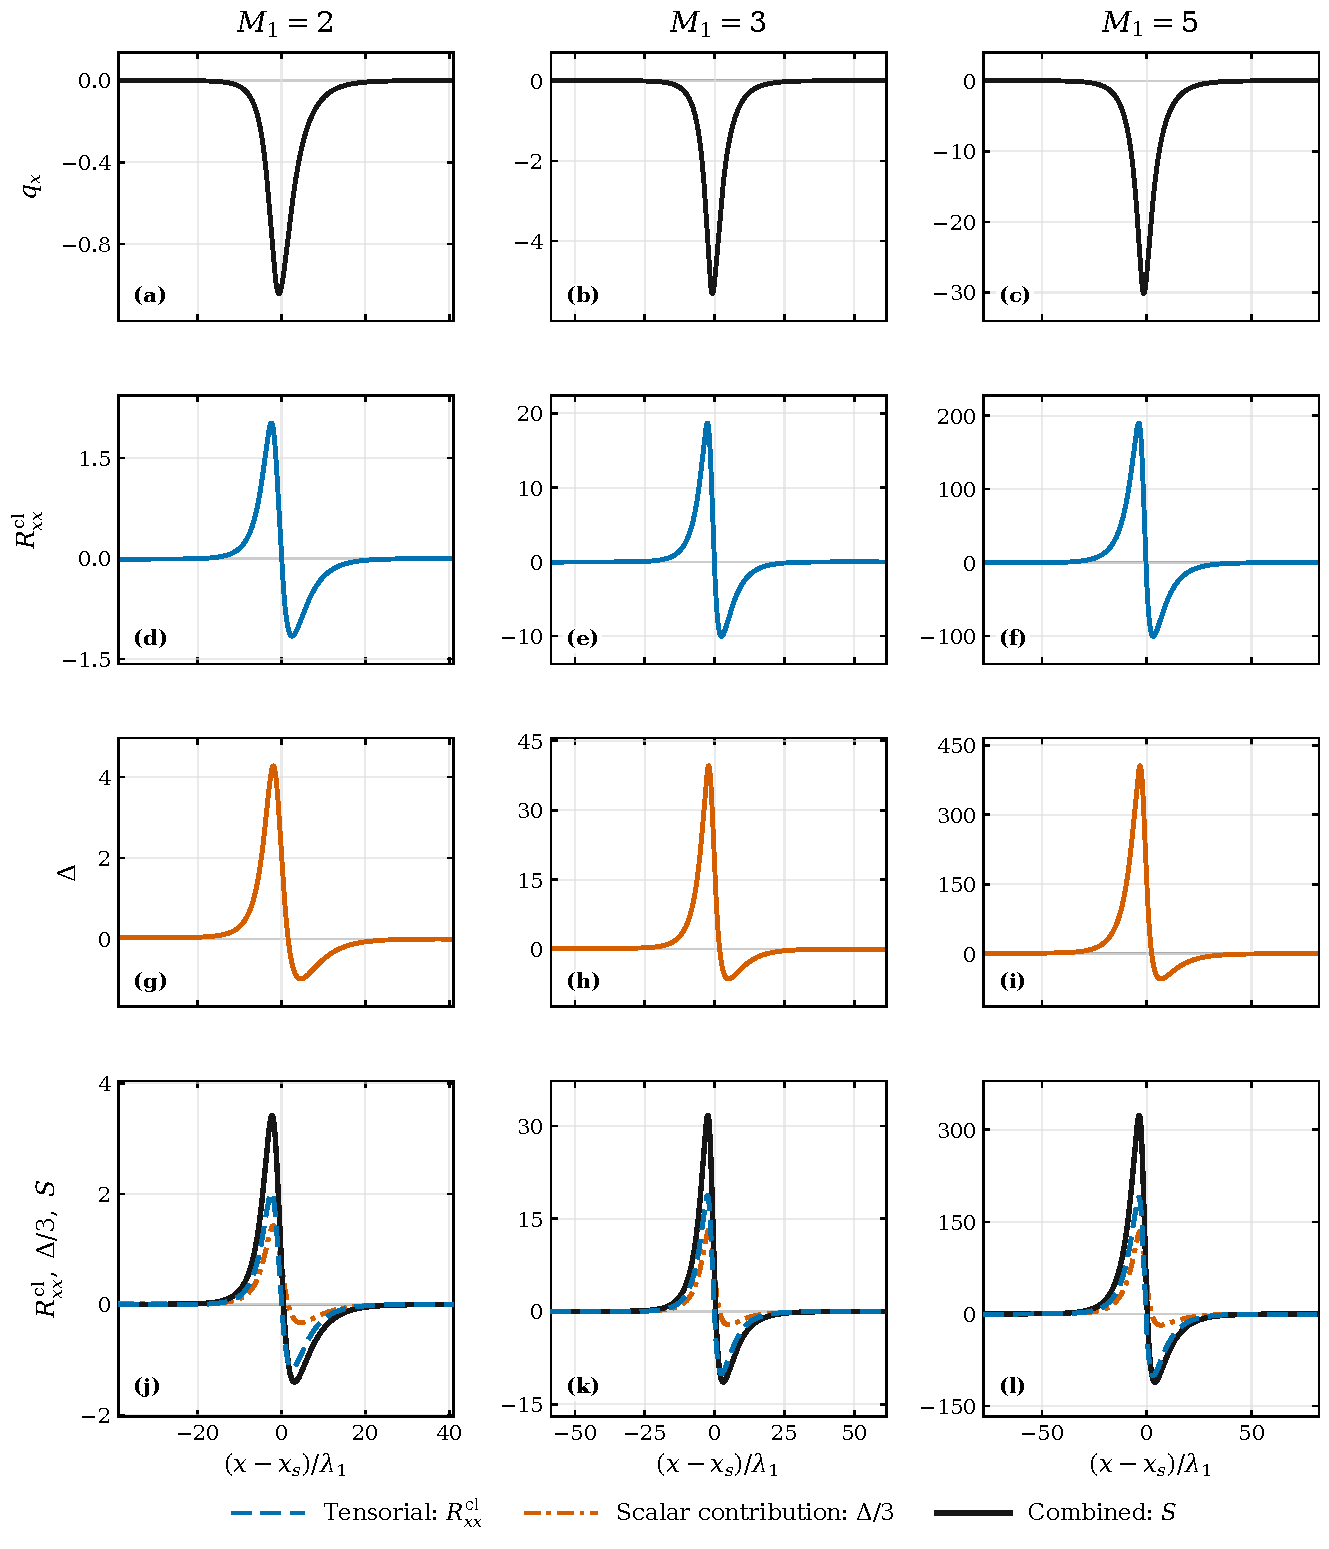
\includegraphics[width=0.98\linewidth]{figures/fig1_dvm_reference.pdf}}
  \caption{Kinetic normal-shock reference profiles at $M_1=2$, 3 and 5. Rows 1--3 show $q_x$, $R^{\cl}_{xx}$ and $\Delta$. The bottom row overlays $R^{\cl}_{xx}$ (blue dashed), $\Delta/3$ (orange dash-dotted) and $S=R^{\cl}_{xx}+\Delta/3$ (black solid) on a common vertical scale within each panel. Vertical scales differ between panels. The archived continuum-reference moments are shown without additional plateau subtraction or smoothing. For this figure, the original plotting convention places $x_s$ at the maximum absolute density gradient, rather than the density midpoint.}
  \label{fig:dvm_ref}
\end{figure}
\clearpage

% Budget source and anchor conventions verified by the deposited full-distribution regeneration.
\section{Exact heat-flux balance and numerical recovery of the observed channel}
\label{sec:heatflux}

\begin{revision}
The identities below state the exact moment balance. The regenerated budget retains the moving-frame contribution and the finite-grid collision source involving $q_x[M_d]-q_x$, and anchors the integrated flux by its directly evaluated value at the first grid point. It uses the same continuum-reference moment definitions and plateau conventions as the scalar-budget reconstruction. The deposited full-distribution checks specify the coordinate, relaxation scale, discrete target and derivative operations; the reported errors refer to this regenerated reconstruction.
\end{revision}

\begin{revision}
For the DVM counterpart of \eqref{eq:bgk}, with $M$ replaced by $M_d$, multiplication by $\frac12|\boldsymbol c|^2c_x$ and integration over velocity give
\begin{equation}
  \partial_x F_q + (\partial_x u_x)\,\mathcal L_q
  =Q_q^{\mathrm{BGK}},
  \qquad
  Q_q^{\mathrm{BGK}}=\frac{q_x[M_d]-q_x[f]}{\Kn} .
  \label{eq:heatbalance_general}
\end{equation}
Here $F_q=\int v_x\psi_q f\,\dd\boldsymbol v$, $\psi_q=|\boldsymbol c|^2c_x/2$, and $\mathcal L_q=\frac12\int v_x(|\boldsymbol c|^2+2c_x^2)f\,\dd\boldsymbol v$. The continuum Maxwellian has $q_x[M]=0$, recovering $Q_q=-q_x/\Kn$. On a fixed finite velocity grid, conservation of density, momentum and energy alone does not impose $q_x[M_d]=0$; its contribution must be evaluated or bounded before using that simplification. The additional term follows from $\partial_x\psi_q=-\frac12(\partial_xu_x)(|\boldsymbol c|^2+2c_x^2)$. It contains moments of order at most three and therefore does not alter the fourth-order observation map. The factor on the right follows from the same $\frac12|\boldsymbol c|^2c_x$ kernel used in the definition of $q_x$. Using the decomposition established in \S\ref{sec:identifiability}, the flux is
\begin{equation}
  F_q=u_xq_x+\frac12\left[B_{xx}[M_d]+7T\sigma_{xx}+S_d\right],
  \qquad S_d=R^{\cl}_{xx}+\Delta_d/3 .
  \label{eq:Bxx_split}
\end{equation}
Here the subscript $d$ emphasises that the budget uses the uncorrected discrete-reference moments. The equilibrium and display-offset conventions are those specified in \S\ref{sec:identifiability}; they must be retained consistently when extracting $S$ from the differential balance.
Explicitly, supplying $Q_q$, $u_x$ and $\mathcal L_q$ gives
\begin{equation}
 F_q(x)=F_q(x_0)+\int_{x_0}^{x}
 \left[Q_q(\xi)-u_x'(\xi)\mathcal L_q(\xi)\right]\,\dd\xi .
 \label{eq:heat_flux_integrated}
\end{equation}
Here $x_0$ is the anchor coordinate, $\xi$ the integration coordinate, and primes on $u_x$ denote spatial derivatives. The flux $F_q(x_0)$ is evaluated from the supplied reference distribution at an anchor point, or from a prescribed full equilibrium distribution when that condition applies. Specifying only incoming reservoir populations does not prescribe the full boundary flux. Equation~\eqref{eq:Bxx_split} then gives $S_d$. One must not impose $S_d=0$ merely because the anchor is called an equilibrium plateau: on a finite grid, $f=M_d$ gives $\Delta_d=0$ but $R^{\cl}_{xx}=-7T\sigma_{xx}[M_d]$, which can be non-zero.

\end{revision}

\begin{revision}
Figure~\ref{fig:budget} compares two ways of evaluating the
same fourth-order channel, $S=R^{\cl}_{xx}+\Delta/3$, for the
Mach-3 BGK reference. The black solid curve, labelled
``full distribution'', is obtained by directly evaluating
the velocity moments defining $R^{\cl}_{xx}$ and $\Delta$
from the saved DVM distribution $f(x,\boldsymbol v)$.
It is therefore a moment profile, not a plot of $f$ itself.

The orange dashed curve, labelled ``integrated heat budget'',
is obtained through the following sequence. Equation~%
\eqref{eq:heatbalance_general} supplies the differential
balance for $F_q$. Equation~\eqref{eq:heat_flux_integrated}
integrates this balance from the first grid point $x_0$,
using the directly evaluated anchor $F_q(x_0)$ and retaining
both the finite-grid source
$Q_q=q_x[M_d]-q_x[f]$ and the moving-frame term
$(\partial_xu_x)\mathcal L_q$ in the present computational
units. Equation~\eqref{eq:Bxx_split} then extracts the
fourth-order channel from the reconstructed flux.
For the continuum-reference moment convention used in
this plot, the resulting expression is
\[
 S_{\rm bud}
 =2\bigl(F_{q,\rm bud}-u_xq_x\bigr)
  -5\rho T^2-7T\sigma_{xx},
\]
with the finite-grid reference offsets treated consistently
before plotting. Both curves use the same display convention:
the mean over the first and last $8\%$ of the spatial samples
is subtracted.

The lower panel evaluates the differential balance using
the directly computed flux, rather than its integrated
reconstruction. Its normalised residual is
\[
 \varepsilon_q(x)=
 \frac{\partial_xF_q-Q_q+
       (\partial_xu_x)\mathcal L_q}
      {\max_x\left|Q_q-(\partial_xu_x)\mathcal L_q\right|}.
\]
Thus, the upper panel checks integrated reconstruction of
$S$, whereas the lower panel checks differential consistency
of the supplied finite-time profile. The reconstruction
uses source and auxiliary moments evaluated from the same
DVM distribution; it is not an independent shock solution
from low-order fields alone. Agreement does not separately
identify $R^{\cl}_{xx}$ and $\Delta$, nor does it by itself
certify stationarity. Separating these two fourth-order
contributions requires the additional scalar budget
introduced in \S\ref{sec:delta_budget}.
\end{revision}

\begin{revision}
The purpose of this comparison is to check the numerical
reconstruction of the observable channel before attempting
to recover its individual components. If the directly
evaluated $F_q$ were merely substituted into
\eqref{eq:Bxx_split}, agreement would follow from the moment
identity. Here, however, the interior flux is reconstructed
by integrating \eqref{eq:heat_flux_integrated}; the direct
flux is used only to supply the anchor at $x_0$.
The comparison therefore tests the combined treatment of
the collision source, moving-frame contribution, integration
and reference offsets. Both evaluations nevertheless use
information from the same DVM distribution, so this is a
consistency check rather than independent validation of the
kinetic model. Its role in the closure-recovery argument is
to establish that $S$ can be reconstructed consistently,
while agreement in $S$ alone cannot distinguish
$R^{\cl}_{xx}$ from $\Delta$. That distinction requires the
additional scalar budget.
\end{revision}

\begin{figure}
  \centerline{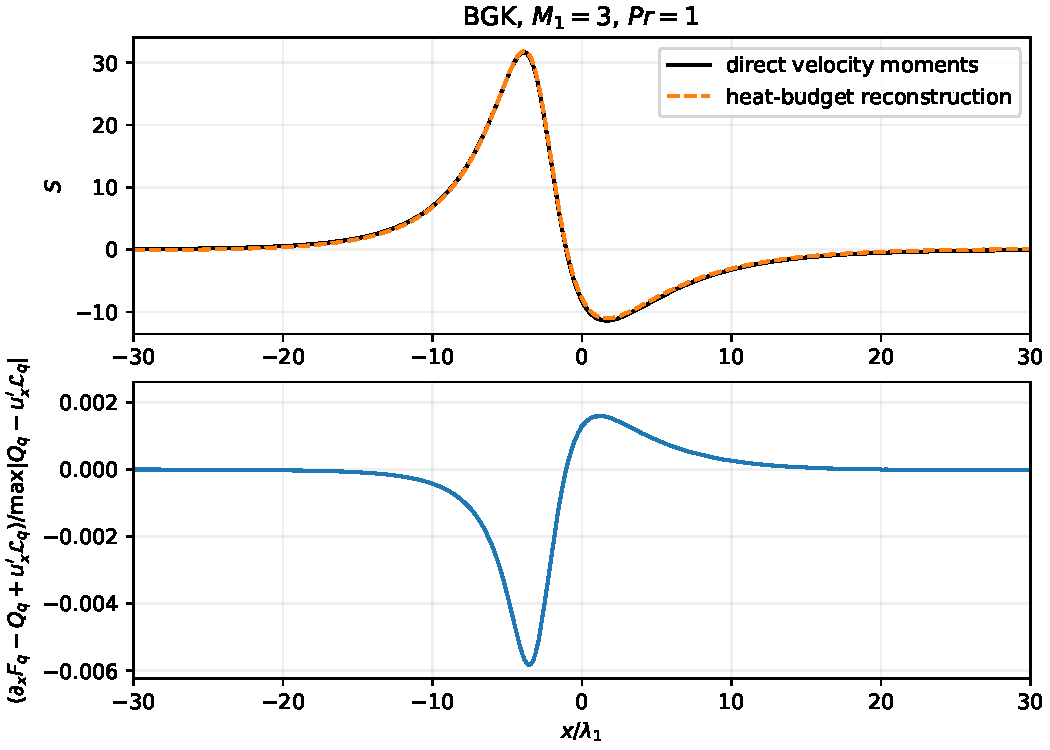
\includegraphics[width=0.97\linewidth]{figures/Figure2_clarified_labels.pdf}}
  \caption{Heat-budget consistency check for the Mach-3 BGK
reference ($Pr=1$). Upper panel: the fourth-order channel
$S=R^{\cl}_{xx}+\Delta/3$ evaluated directly from the full
DVM distribution (black solid) and reconstructed by
integrating the heat-flux balance and extracting $S$
through \eqref{eq:Bxx_split} (orange dashed). Both profiles
use the same plateau subtraction. Lower panel: the
normalised differential residual $\varepsilon_q$, defined
in the text, evaluated with the directly computed $F_q$.
Here $Q_q=q_x[M_d]-q_x[f]$ and
$\mathcal L_q=\int v_x(\tfrac12|\boldsymbol c|^2+c_x^2)
f\,\dd\boldsymbol v$.
The symbol $A$ in the plotting data denotes this same
$\mathcal L_q$; its multiplier is the velocity gradient
$\partial_xu_x$, not the velocity $u_x$.
The comparison tests reconstruction and differential
consistency, not independent closure recovery or
certified stationarity.}
  \label{fig:budget}
\end{figure}

\newpage
\section{\revisionheading{Scalar-excess budget and two-channel recovery}}
\label{sec:delta_budget}

\begin{revision}
The missing channel is supplied by a scalar fourth-order budget.  Multiplication of \eqref{eq:bgk} by $|\boldsymbol c|^4$ gives
\begin{equation}
  \int |\boldsymbol c|^4 v_x\partial_x f\,\dd\boldsymbol v = Q_\Delta .
  \label{eq:delta_raw}
\end{equation}
Because the peculiar velocity depends on the local velocity $u_x(x)$, the flux derivative contains a moving-frame contribution.  Define
\begin{equation}
  J_\Delta=\int v_x|\boldsymbol c|^4 f\,\dd\boldsymbol v,
  \qquad
  K_\Delta=\int v_x|\boldsymbol c|^2 c_x f\,\dd\boldsymbol v .
  \label{eq:J_K_delta}
\end{equation}
These fluxes specify what additional information is needed. In fact $K_\Delta=2F_q$, whereas
\[
 J_\Delta=u_x\int |\boldsymbol c|^4f\,\dd\boldsymbol v
             +\int c_x|\boldsymbol c|^4f\,\dd\boldsymbol v
\]
contains a fifth-order moment not determined by the lower-order fields and $S$. Here these fluxes are evaluated from the full DVM distribution: the two-budget procedure tests moment recovery and consistency, rather than defining a closed solver from low-order data alone. Since $\partial_x|\boldsymbol c|^4=-4|\boldsymbol c|^2c_x\partial_xu_x$, one obtains
\begin{equation}
  \int |\boldsymbol c|^4 v_x\partial_x f\,\dd\boldsymbol v
  =\partial_x J_\Delta+4(\partial_xu_x)K_\Delta .
  \label{eq:delta_flux_identity}
\end{equation}
For BGK, the collision source is
\begin{equation}
  Q_\Delta^{\mathrm{BGK}}=\frac{1}{\Kn}\int |\boldsymbol c|^4(M_d-f)\,\dd\boldsymbol v=-\frac{\Delta_d}{\Kn} ,
  \label{eq:delta_bgk_source}
\end{equation}
where in the DVM implementation $M\to M_d$. The identity is exact for the uncorrected discrete excess $\Delta_d$ in \eqref{eq:Deltadef}; use of a plateau-corrected $\Delta$ requires the same correction in the source. Thus the raw budget reconstructs $\Delta_d$. A displayed field $\Delta=\Delta_d-o_\Delta$ instead satisfies $Q_\Delta=-(\Delta+o_\Delta)/\Kn$ and requires subtracting $o_\Delta$ from the reconstructed excess. Hence
\begin{equation}
  \Delta_{d,\rm bud}=-\Kn\left[\partial_xJ_\Delta+4(\partial_xu_x)K_\Delta\right].
  \label{eq:delta_rec}
\end{equation}
The scalar-budget derivative uses a centred seven-point boxcar on the moment inputs, with the same convention for the Mach-2, Mach-3 and Mach-5 reconstructions. 
\end{revision}

\begin{revision}
The form of the scalar-excess source depends on the collision operator, but the flux-side observation operator does not.  For a generic kinetic equation $v_x\partial_x f=\mathcal C[f]$, the heat-flux source is
\begin{equation}
  Q_q=\int \frac12 |\boldsymbol c|^2 c_x\,\mathcal C[f]~\dd\boldsymbol v,
  \qquad
  Q_\Delta=\int |\boldsymbol c|^4\,\mathcal C[f]~\dd\boldsymbol v .
  \label{eq:generic_sources}
\end{equation}
The source changes with the collision model, while the observed fourth-order channel in the heat-flux flux remains the same kinematic projection. Recovering $\Delta$ from a budget requires a source law invertible for $\Delta$ once its other inputs are supplied; a general Boltzmann production measurement alone is not such an algebraic inversion. The analytic Shakhov, ES-BGK and ES-FP source laws below use full velocity-space integrals and the continuum-reference excess $\Delta=\Delta_c$, without plateau subtraction. Discrete-reference diagnostics require the corresponding equilibrium-offset corrections; finite-box Fokker--Planck evaluations also require boundary and discretisation checks.  BGK gives \eqref{eq:delta_bgk_source}.  The Shakhov target changes the heat-flux moment so that $Q_q=-Pr\,q_x/\Kn$, but its correction is odd in $\boldsymbol c$ and integrates to zero against the even kernel $|\boldsymbol c|^4$; therefore $Q_\Delta=-\Delta/\Kn$ is unchanged. This parity proof applies on full velocity space (or a domain symmetric in $\boldsymbol c$). A fixed laboratory-frame grid is generally not symmetric about the local $u_x$; discrete neutrality must be evaluated for the actual target and quadrature rather than inferred from this continuum argument. Thus a correct-Prandtl Shakhov correction alters the heat-flux relaxation without changing the scalar-excess source.
\end{revision}

\begin{revision}
Unlike Shakhov, ES-BGK uses an anisotropic Gaussian target \citep{Holway1966ESBGK,FeiLiuLiuZhang2020ShockBenchmark},
\begin{equation}
  G_\Theta(\boldsymbol c)
  =\frac{\rho}{(2\pi)^{3/2}(\det\Theta)^{1/2}}
  \exp\left[-\frac12 c_i(\Theta^{-1})_{ij}c_j\right],
  \label{eq:es_gaussian}
\end{equation}
with covariance tensor $\Theta$.
 The operators $\det$ and $\tr$ denote determinant and trace.
The dimensionless coefficient $\alpha_{\rm ES}$ controls target anisotropy.  In the conventional monatomic ES-BGK construction, $\Theta=T I+\Lambda_{\rm ES}$, where $\Lambda_{\rm ES}$ is a trace-free tensor proportional to the stress; in the notation used here one may write $\Lambda_{\rm ES}=\alpha_{\rm ES}\sigma/\rho$ with the stress convention defined above. Here $T$ is the local scalar temperature in the adopted
units ($R=1$), and $I$ is the $3\times3$ identity tensor;
thus $TI$ represents the isotropic part of the
velocity covariance. The heat-flux observation channel does not change, because it is determined by the left-hand-side flux.  The scalar-excess source does change, because the target distribution no longer has the Maxwellian fourth scalar moment.
\end{revision}

\begin{revision}
For any zero-mean Gaussian with covariance $\Theta$,
\begin{equation}
  \int |\boldsymbol c|^4G_\Theta\,\dd\boldsymbol v
  =\rho\left[(\tr\Theta)^2+2\tr(\Theta^2)\right].
  \label{eq:es_fourth}
\end{equation}
This identity follows from Wick's theorem:
 the brackets here denote expectation under the normalised Gaussian $G_\Theta/\rho$; $\langle c_i c_i c_j c_j\rangle=(\tr\Theta)^2+2\tr(\Theta^2)$.  For a Maxwellian, $\Theta=T I$, so $(\tr\Theta)^2=9T^2$ and $2\tr(\Theta^2)=6T^2$, giving $15T^2$.  For ES-BGK, however, the trace-free part $\Lambda_{\rm ES}$ gives
\begin{equation}
  \Delta_G^{\rm ES}
  =\rho\left[(\tr\Theta)^2+2\tr(\Theta^2)-15T^2\right]
  =2\rho\,\tr(\Lambda_{\rm ES}^2)
  =\frac{2\alpha_{\rm ES}^2}{\rho}\tr(\sigma^2).
  \label{eq:es_delta_target}
\end{equation}
Thus the ES-BGK scalar-excess source is not simply $-\Delta/\Kn$, but
\begin{equation}
  Q_\Delta^{\rm ES-BGK}
  =\frac{1}{\Kn}\left(\Delta_G^{\rm ES}-\Delta\right) .
  \label{eq:es_delta_source}
\end{equation}
In a one-dimensional normal shock, $\sigma_{yy}=\sigma_{zz}=-\sigma_{xx}/2$, so $\tr(\sigma^2)=3\sigma_{xx}^2/2$ and
\begin{equation}
  \Delta_G^{\rm ES}=\frac{3\alpha_{\rm ES}^2}{\rho}\sigma_{xx}^2 .
  \label{eq:es_1d_delta_target}
\end{equation}
This term is nonnegative: the ES-BGK target carries a non-zero scalar fourth-order excess whenever the covariance is anisotropic.  Shakhov changes the odd heat-flux channel and leaves the even $|\boldsymbol c|^4$ channel neutral; ES-BGK changes the even scalar-excess target through a stress-squared covariance effect.
\end{revision}


To estimate the size of this correction in the present shocks, we post-process the Mach 2, 3 and 5 DVM profiles using \eqref{eq:es_1d_delta_target} with $Pr=2/3$ and $\alpha_{\rm ES}=1-1/Pr=-1/2$.  Table~\ref{tab:model_source_corrections} reports the relative
magnitude $\|\Delta_G^{\rm ES}\|/\|\Delta\|$ of the
stress-dependent target excess. Here ``correction'' denotes
the additional contribution $\Delta_G^{\rm ES}/\Kn$ to the
BGK scalar-excess source $-\Delta/\Kn$. The ratio $\|\Delta_G^{\rm ES}\|/\|\Delta\|$ in the active shock layer is approximately $4.3$--$4.5\%$ for all three Mach numbers, and the ES-BGK scalar-excess source remains almost collinear with the BGK/Shakhov source, with correlations exceeding $0.999$.  The correction is therefore modest on these evaluated BGK profiles, but it is systematically non-zero and grows in absolute magnitude with Mach number: the peak value of $\Delta_G^{\rm ES}$ increases from $0.196$ at $M_1=2$ to $20.25$ at $M_1=5$.  These percentages describe source evaluations on the stored BGK profiles, not independently evolved ES-BGK fields. We additionally implement and evolve the ES-BGK kinetic model itself at Mach 2 and 3, with $Pr=2/3$ and transport matched to the Shakhov campaign. Appendix~\ref{app:esbgk_evolved} reports its solver, finite-time profiles and two-budget reconstructions. The source-only comparison in table~\ref{tab:model_source_corrections} and figure~\ref{fig:esfp_esbgk_sources} is retained as a controlled comparison on common input fields; ES-FP remains a post-processing diagnostic.

\begin{revision}
Fokker--Planck models provide a complementary example because their sources are generated by drift and diffusion rather than by relaxation to a target distribution.  For a velocity-space Fokker--Planck operator
\begin{equation}
  \mathcal C_{\rm FP}[f]
  =-\partial_{c_i}(A_i f)+\frac12\partial_{c_i}\partial_{c_j}(D_{ij}f),
  \label{eq:fp_operator}
\end{equation}
two integrations by parts on full velocity space, with sufficiently decaying distributions and vanishing boundary terms, transfer the derivatives to $\phi=|\boldsymbol c|^4$. Since $\partial_{c_i}\phi=4|\boldsymbol c|^2c_i$ and $\partial_{c_i}\partial_{c_j}\phi=8c_ic_j+4|\boldsymbol c|^2\delta_{ij}$, the scalar production is
\begin{equation}
  Q_\Delta^{\rm FP}
  =\int \left[4A_i|\boldsymbol c|^2c_i+4D_{ij}c_i c_j+2D_{ii}|\boldsymbol c|^2\right]f~\dd\boldsymbol v .
  \label{eq:fp_delta_source_general}
\end{equation}
This form is useful because it makes the difference from BGK-type relaxation explicit.  In an ES-FP model with standard linear drift $A_i=-\nu c_i$ and anisotropic diffusion $D_{ij}=2\nu(T\delta_{ij}+\beta\sigma_{ij}/\rho)$, substitution gives
\begin{equation}
  Q_\Delta^{\rm ES-FP}
  =\nu\left[-4\Delta+\frac{8\beta}{\rho}\tr(\sigma^2)\right]
  =4\nu\left[-\Delta+\frac{2\beta}{\rho}\tr(\sigma^2)\right].
  \label{eq:esfp_delta_source}
\end{equation}
Here $A_i$ is the velocity-space drift, $D_{ij}$ the diffusion tensor,
$\nu>0$ the collision-rate scale and $\beta$ the dimensionless
diffusion-anisotropy coefficient. The fourth-order test function is
$\phi(\boldsymbol c)=|\boldsymbol c|^4$.

For the correct-Prandtl choice $\beta=-5/4$, the ES-FP correction is therefore proportional to the same stress-squared invariant as the ES-BGK correction, but with a different coefficient and opposite sign. For clarity, substitution of $\int c_ic_jf\,\dd\boldsymbol v=\rho T\delta_{ij}+\sigma_{ij}$ and $\tr\sigma=0$ gives
\[
 \frac{Q_\Delta}{\nu}
 =-4(\Delta+15\rho T^2)+24\rho T^2+36\rho T^2
   +\frac{8\beta}{\rho}\tr(\sigma^2).
\]
The equilibrium terms cancel, yielding \eqref{eq:esfp_delta_source} before any normal-shock symmetry reduction. On a finite velocity box the discarded boundary terms require a separate check. This formal source identity presupposes an admissible diffusion tensor. With $\mathsf C=\rho^{-1}\int\boldsymbol c\boldsymbol c f\,\dd\boldsymbol v=TI+\sigma/\rho$ the actual distribution covariance, its normalised form is $D/(2\nu)=(1-\beta)TI+\beta\mathsf C$. At $\beta=-5/4$, positive definiteness requires every eigenvalue of $\mathsf C$ to be smaller than $9T/5$. A fixed correct-Prandtl coefficient does not guarantee this condition for arbitrary nonequilibrium states.  Entropy inequalities for Gaussian ES-BGK and admissible ES-FP models are established in the literature \citep{Andries2000GaussianBGK,MathiaudMieussens2016ESFP}. In particular, the latter allows a state-dependent anisotropy parameter to maintain admissible diffusion; a fixed $\beta=-5/4$ cannot be extended to arbitrary far-from-equilibrium states. Those results are distinct from our sampled finite-grid entropy diagnostic. This is the scalar-excess analogue of the high-order-moment production differences emphasised in shock-wave benchmark studies of BGK, Shakhov, ES-BGK, ES-FP and Cubic-FP models \citep{FeiLiuLiuZhang2020ShockBenchmark}.  It also explains why equal Prandtl number does not imply equal fourth-order closure production: the heat-flux relaxation rate is a lower-order transport constraint, whereas $Q_\Delta$ samples an even fourth-order kernel.
\end{revision}

\begin{revision}
The constant source-correction ratio follows directly from this algebra, not from a separate numerical fit.  After the ES-FP source is scaled by $4\nu$, its stress-quadratic correction is
\begin{equation}
  Q_{\Delta,\mathrm{corr}}^{\rm ES-FP}/(4\nu)
  =\frac{2\beta}{\rho}\tr(\sigma^2),
\end{equation}
whereas the ES-BGK correction from \eqref{eq:es_delta_target} is
\begin{equation}
  \Delta_G^{\rm ES}
  =\frac{2\alpha_{\rm ES}^2}{\rho}\tr(\sigma^2).
\end{equation}
Equivalently, $Q_{\Delta,\mathrm{corr}}^{\rm ES-FP}/(4\nu)=(\beta/\alpha_{\rm ES}^2)\Delta_G^{\rm ES}$ for $\alpha_{\rm ES}\ne0$. Wherever $\Delta_G^{\rm ES}\ne0$, their pointwise ratio is
\begin{equation}
  \frac{Q_{\Delta,\mathrm{corr}}^{\rm ES-FP}/(4\nu)}{\Delta_G^{\rm ES}}
  =\frac{\beta}{\alpha_{\rm ES}^2}.
  \label{eq:esfp_esbgk_ratio}
\end{equation}
For $Pr=2/3$, $\alpha_{\rm ES}=1-1/Pr=-1/2$ and $\beta=-5/4$, so \eqref{eq:esfp_esbgk_ratio} gives exactly $-5$.  The ratio $-5$ is therefore an analytical consequence of the ES-BGK Gaussian covariance and ES-FP anisotropic diffusion coefficients; the DVM post-processing only measures the size of the common stress-squared invariant relative to the actual shock-layer $\Delta$.
\end{revision}

Table~\ref{tab:model_source_corrections} and figure~\ref{fig:esfp_esbgk_sources} compare the ES-BGK and ES-FP source-level diagnostics on the same DVM shock profiles.  The ES-FP correction contributes $21.5\%$, $22.4\%$ and $22.0\%$ of $\|\Delta\|$ for Mach 2, 3 and 5, respectively, about five times the ES-BGK correction in magnitude and with the opposite sign for $\beta=-5/4$.  Nevertheless, the full scaled ES-FP source remains strongly aligned with the BGK/Shakhov scalar-excess source, with correlations $0.987$, $0.984$ and $0.984$.  Thus ES-FP does not change the kinematic observation channel; it changes the source that drives the missing scalar complement.  This distinction is central to the paper: $S$ is the channel observed by the heat-flux flux, while $Q_\Delta$ is the collision-model-specific mechanism by which the scalar-excess information is produced.

\begin{table}
  \centering
\revisionbox{\begin{minipage}{0.96\textwidth}\captionsetup{width=\linewidth}
  \caption{Source-level ES-BGK and ES-FP scalar-excess corrections evaluated on the DVM shock profiles.  The ratios are active-zone norms relative to $\|\Delta\|$.  The opposite signs reflect different mechanisms: anisotropy raises the fourth scalar moment of the ES-BGK Gaussian target, whereas the ES-FP correction contracts the stress with anisotropic diffusion. At $Pr=2/3$, $\beta/\alpha_{\rm ES}^2=-5$; this is a source coefficient ratio, not an entropy-production sign. The ES-FP source is the scaled source $Q_\Delta^{\rm ES-FP}/(4\nu)$ in \eqref{eq:esfp_delta_source}; the correlation compares the full ES-FP scaled source with the BGK/Shakhov baseline $-\Delta$.}
  \label{tab:model_source_corrections}
  \begin{tabular}{lrrr}
  \toprule
  Mach & ES-BGK correction & ES-FP correction & corr$(Q_\Delta^{\rm ES-FP},-\Delta)$\\
  \midrule
  M2 & 0.0431 & 0.215 & 0.987\\
  M3 & 0.0447 & 0.224 & 0.984\\
  M5 & 0.0439 & 0.220 & 0.984\\
  \bottomrule
  \end{tabular}
  \end{minipage}}\par
\end{table}

\begin{figure}
  \centerline{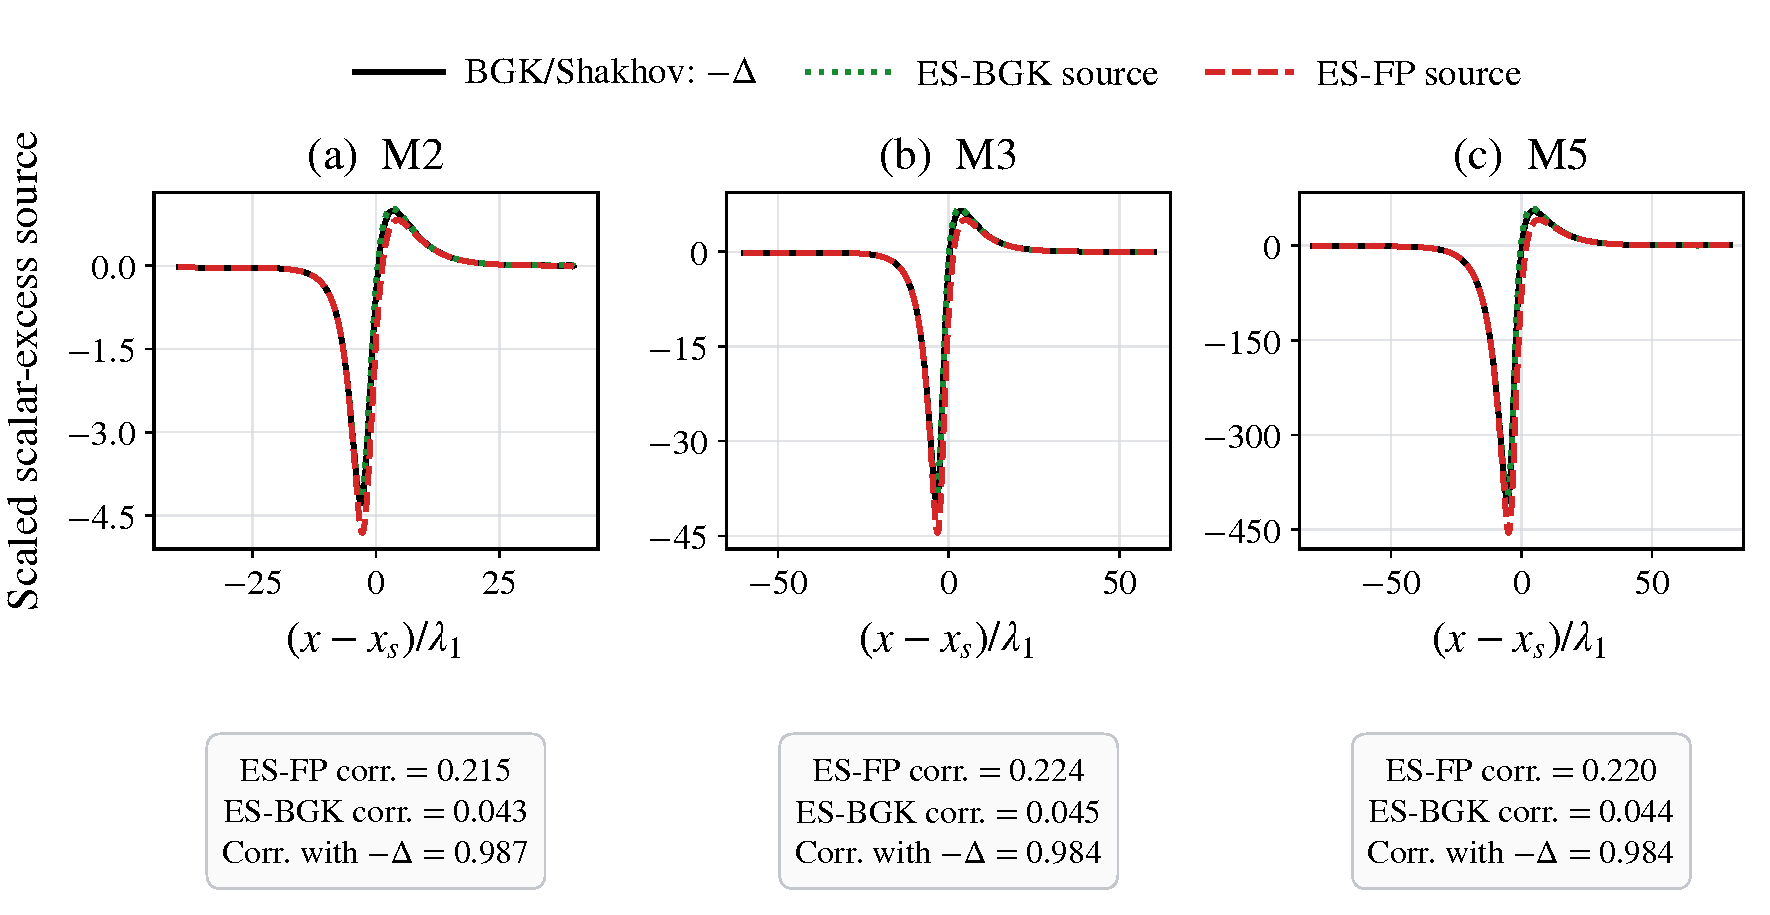
\includegraphics[width=0.98\linewidth]{figures/Figure3_large_fonts.pdf}}
  \caption{Scaled scalar-excess source for BGK/Shakhov, ES-BGK and ES-FP, evaluated on the Mach 2, 3 and 5 DVM shock profiles.  The black curve is the BGK/Shakhov baseline $-\Delta$.  ES-BGK gives a small stress-quadratic correction from the anisotropic Gaussian target, whereas ES-FP gives a larger anisotropic-diffusion correction of opposite sign.  The nearly coincident shapes show that the source remains strongly aligned with the scalar-excess channel, while the separation between green and red curves shows that correct-Prandtl kinetic models can assign different fourth-order production laws to the same observed heat-flux channel.}
  \label{fig:esfp_esbgk_sources}
\end{figure}

This result is consistent with benchmark studies showing that correct-Prandtl kinetic models can agree in low-order transport while differing in higher-order moments and their production terms in shock waves \citep{FeiLiuLiuZhang2020ShockBenchmark}.  In the present language, ES-BGK changes the scalar-excess source through a stress-quadratic target term, ES-FP changes it more strongly through anisotropic diffusion, and Shakhov does not change it at all.  These differences are invisible if one looks only at density, velocity, stress or heat-flux relaxation rates.  They become visible only after the scalar-excess channel has been identified as the missing complement to the heat-flux observation channel.

\subsection{Shakhov source-neutrality and channel-consistency check}
\label{sec:shakhov}

\begin{revision}
The Shakhov model is the most direct correct-Prandtl test of the BGK result because it changes the heat-flux relaxation without replacing the Maxwellian covariance by an anisotropic one.  We therefore evaluate a conservative discrete Shakhov target \citep{Shakhov1968} on the Mach-3 DVM shock.  The Shakhov target, denoted $M_S$, has the form of a Maxwellian multiplied by an odd heat-flux correction.  Consequently the odd correction contributes to the heat-flux projection but vanishes against the even scalar kernel $|\boldsymbol c|^4$; the target retains the Maxwellian scalar fourth moment.  Numerically, the target gives $q_x[M_S]/q_x[f]=0.333323\simeq 1-Pr$ and the direct heat-flux collision source gives $Q_q/q_x[f]=-0.666677\simeq -Pr$, as required for $Pr=2/3$.  At the same time, the evaluated scalar-excess source remains $Q_\Delta=-\Delta/\Kn$ to numerical precision for this target and grid; this is a numerical check of the discrete construction.  
\end{revision}

\begin{revision}
This check is deliberately not another spatial budget reconstruction.  It evaluates the collision projections directly from the discrete distribution and therefore isolates the channel identity from the finite-difference derivative error present in figures~\ref{fig:two_budget} and \ref{fig:sparse_delta}.  Figure~\ref{fig:shakhov_check} shows that the heat-flux flux reconstructs $S$ with a $0.064\%$ active-zone error, the scalar-excess channel reconstructs $\Delta$ to numerical precision, and the two-channel recovery reduces the $R^{\cl}_{xx}$ error from $68.4\%$ to $0.10\%$.  This source-neutrality verification shows that the heat-flux observation channel and scalar-excess complement survive correction of the Prandtl-number defect of BGK; it does not introduce a new recovery method.
\end{revision}

\begin{figure}
  \centerline{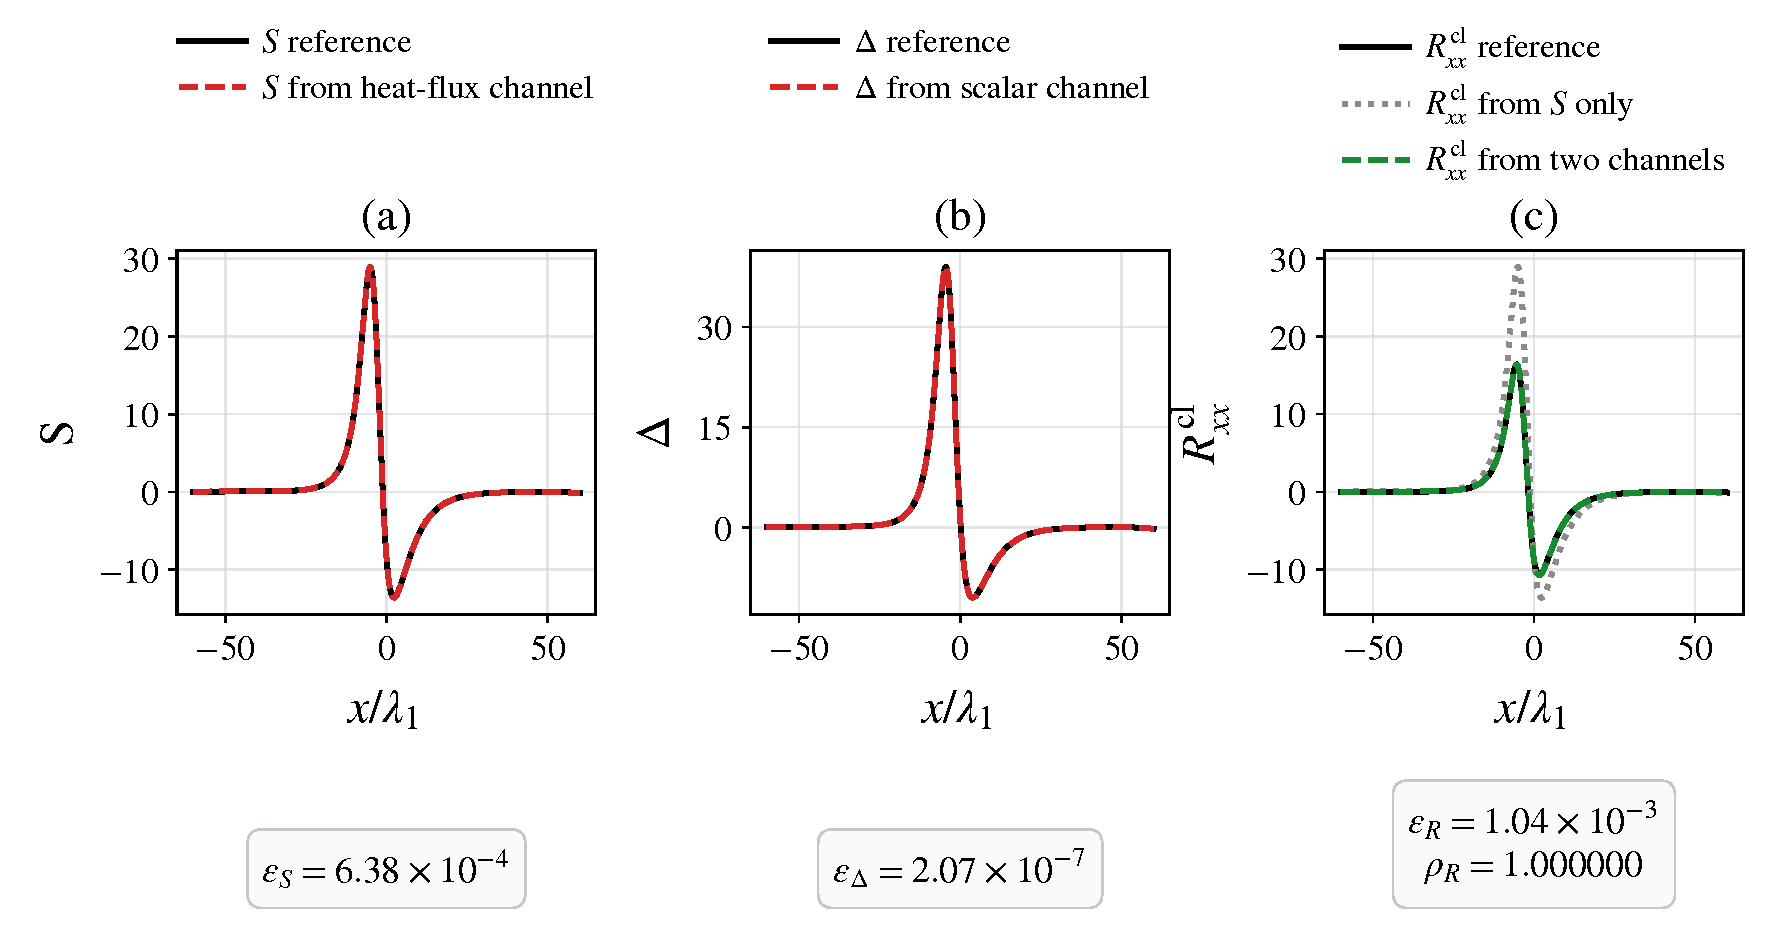
\includegraphics[width=0.99\linewidth]{figures/Figure4_large_fonts.pdf}}
  \caption{Conservative discrete Shakhov channel check for the Mach-3 shock with $Pr=2/3$. (a) The heat-flux flux channel reconstructs $S$. (b) The scalar-excess source is neutral under the Shakhov correction and recovers $\Delta$. (c) The heat-flux channel alone gives a large $R^{\cl}_{xx}$ error, whereas the two-channel reconstruction recovers the tensorial closure moment. The panel errors are relative norms expressed as fractions. The collision sources are evaluated directly from the discrete distribution, so this checks channel consistency rather than replacing the BGK spatial budget sweep in figures~\ref{fig:two_budget} and \ref{fig:sparse_delta}.}
  \label{fig:shakhov_check}
\end{figure}

\begin{revision}
The check uses $Pr=2/3$ and a unit computational source scale. The distribution minimum is near $10^{-30}$, while the signed target minimum is approximately $-9.96\times10^{-5}$; the collision projection therefore does not certify a nonnegative Shakhov target or a stationary shock. Each displayed reference and reconstructed channel has the mean of the first and last $8\%$ of points removed, with active mask $|S|>0.02\max|S|$. The agreement in the scalar channel is plateau-corrected: $\Delta_{\rm source}+\Kn Q_\Delta$ is a constant offset, approximately $0.06816$. The flux-side subtraction uses $5\rho T^2$, whereas the directly evaluated closure moments use $f-M_d$, so the small flux-channel discrepancy also contains the discrete Maxwellian reference defect. The numerical curves have been regenerated from the archived full distribution; the input, code, profiles and provenance are deposited with the article.
\end{revision}



\begin{revision}
A separate short diagnostic compares clipped and signed Shakhov updates for 20 sweeps from the same initial state. Relative differences in $R$, $\Delta$ and $S$ are approximately $1.335\%$, $1.547\%$ and $1.465\%$. This finite-sweep comparison does not establish a steady solution for either branch, but it prevents treating positivity clipping as numerically neutral. The analytic odd-parity source-neutrality statement concerns the unmodified collision correction; it must be distinguished from conservation and source balances after clipping.
\end{revision}

\subsection{Boltzmann limit and direct DSMC production}
\label{sec:model_ladder_boltzmann}

\begin{revision}
For the Boltzmann collision operator, the analogue is the genuine collision-production integral $\int |\boldsymbol c|^4 Q(f,f)\,\dd\boldsymbol v$.  In DSMC this production can be accumulated directly by summing the change of $|\boldsymbol c|^4$ over accepted binary collisions.  The hierarchy of sources is therefore: BGK and Shakhov give a scalar relaxation of $\Delta$; ES-BGK adds a stress-squared target excess; ES-FP modifies the same channel through anisotropic diffusion; and the Boltzmann operator defines the fourth-order production, which DSMC estimates from molecular collisions.  In all cases, however, the flux-side heat-flux observation operator remains the same composite fourth-order channel.  The DSMC test in \S\ref{sec:dsmc} closes this loop by measuring the scalar-excess production directly in a stochastic binary-collision shock.
\end{revision}

\begin{revision}

Table~\ref{tab:source_laws} separates the common kinematic channel $S$ from the model-dependent scalar production $Q_\Delta$. This distinction allows the same observation map to be tested with different collision-source laws.
\end{revision}

\begin{table}
  \begin{center}
  \caption{Observation channel and fourth-order source laws for the models considered here.  The heat-flux observation channel is kinematic, whereas the source laws are collision-model dependent.  The analytic relaxation formulas use continuum-reference moments on full velocity space; discrete equilibrium and quadrature corrections are as described in the text. Here $\psi_q=\frac12 |\boldsymbol c|^2c_x$, $G_\Theta$ is the ES-BGK anisotropic Gaussian, $A_i$ and $D_{ij}$ are Fokker--Planck drift and diffusion coefficients, and $Q(f,f)$ is the Boltzmann collision operator.}
  \label{tab:source_laws}
  \begin{tabular}{p{0.17\textwidth}p{0.22\textwidth}p{0.23\textwidth}p{0.25\textwidth}}
  \toprule
  Model & Heat-flux source $Q_q$ & Scalar-excess source $Q_\Delta$ & Interpretation\\
  \midrule
  BGK & $-q_x/\Kn$ & $-\Delta/\Kn$ & Baseline relaxation of heat flux and scalar excess.\\
  Shakhov & $-Pr\,q_x/\Kn$ & $-\Delta/\Kn$ & Corrects heat-flux relaxation; odd Shakhov correction is neutral in the even $|\boldsymbol c|^4$ channel.\\
  ES-BGK & target-dependent & $(\Delta_G^{\rm ES}-\Delta)/\Kn$ & Anisotropic covariance adds a stress-quadratic scalar-excess target.\\
  ES-FP & drift/diffusion dependent & $\nu[-4\Delta+8\beta\tr(\sigma^2)/\rho]$ & Anisotropic diffusion changes the scalar-excess production even when the Prandtl number is corrected.\\
  Boltzmann/DSMC & $\int \psi_q Q(f,f)\,\dd\boldsymbol v$ & $\int |\boldsymbol c|^4 Q(f,f)\,\dd\boldsymbol v$ & True collisional production; sampled in DSMC from pre/post-collision changes of $|\boldsymbol c|^4$.\\
  \bottomrule
  \end{tabular}
  \end{center}
\end{table}

\subsection{\revisionheading{Numerical two-budget recovery across Mach number}}
\label{sec:two_budget}

\begin{revision}
The closure recovery now follows directly.  The heat-flux budget gives $S$, the scalar-excess budget gives $\Delta_{\rm bud}$, and the tensorial closure is reconstructed as
\begin{equation}
  R^{\cl}_{xx,\rm bud}=S_{\rm bud}-\Delta_{\rm bud}/3 .
  \label{eq:two_budget_R}
\end{equation}

The numerical budgets use the actual discrete velocity weights and retain the Maxwellian target moments in the collision contractions. In particular, $Q_q=(q_x[M_d]-q_x[f])/\tau$ and the scalar reconstruction is
\begin{equation}
\Delta_{\rm bud}
=
\sum_k w_k|\boldsymbol c_k|^4 M_{d,k}
-15\rho T^2
-\tau\left(
\frac{\mathrm dJ_\Delta}{\mathrm dx}
+4\frac{\mathrm du_x}{\mathrm dx}K_\Delta
\right).
\end{equation}

Here $k$ indexes the discrete three-dimensional velocity nodes
$\boldsymbol v_k$, $w_k$ denotes their velocity-quadrature weights,
and $\boldsymbol c_k=\boldsymbol v_k-u_x\boldsymbol e_x$ is the
peculiar velocity at node $k$, with $\boldsymbol e_x$ the unit vector
in the shock-normal direction. The quantity $M_{d,k}$ is the
conservative discrete Maxwellian target evaluated at that node,
matching the density, momentum and energy of the local discrete
distribution. The fields $\rho$, $u_x$ and $T$ are the local density,
streamwise mean velocity and temperature, respectively; temperature
is expressed in the computational convention $R=1$.
The parameter $\tau$ is the BGK relaxation time, equal to one in
the computational units used for these budget reconstructions.
The two fluxes are evaluated with the same quadrature:
\[
J_\Delta=\sum_k w_k v_{x,k}|\boldsymbol c_k|^4 f_k,
\qquad
K_\Delta=\sum_k w_k v_{x,k}|\boldsymbol c_k|^2c_{x,k}f_k,
\]
where $f_k=f(x,\boldsymbol v_k)$.\par\end{revision}\begin{revision}
Thus $\Delta_{\rm bud}$ reconstructs the continuum-reference
scalar excess
$\Delta_c=\sum_k w_k|\boldsymbol c_k|^4f_k-15\rho T^2$,
before the subsequent plateau subtraction.

Suffixes $d$ and $c$
refer to discrete and continuum equilibrium, respectively;
$\rm bud$, $\rm full$ and $\rm sparse$ identify budget reconstruction,
complete scalar-field input and interpolated probe input.
Macroscopic fields are recomputed consistently from the stored distribution, and the conservative discrete target is evaluated in double precision with four matching iterations. The heat-flux integral is anchored by its directly evaluated value at the first grid point. With the stored \texttt{x\_mfp} coordinate, computational $\tau=1$ is used. Derivatives employ one $(1,4,6,4,1)/16$ pass on $u_x$ for the heat budget and a seven-point boxcar on $J_\Delta,u_x,K_\Delta$ for the scalar budget. The raw discrete-source inversion reconstructs $\Delta_d$. Adding the local offset $\sum_k w_k|\boldsymbol c_k|^4M_{d,k}-15\rho T^2$ converts it to $\Delta_c$ before the stated plateau subtraction. The heat-flux channel subtracts the continuum term $5\rho T^2$; it retains the directly evaluated $q_x[M_d]$ in the source and the measured first-point flux anchor. The tensorial reference likewise omits the discrete-Maxwellian fourth-moment subtraction. These choices put both reconstructed channels and their reference on the same continuum-reference convention. These budget checks do not establish stationarity or independent grid convergence.

\textbf{Error measures and comparison sets.} For a reconstruction $g_{\rm rec}$ and reference $g_{\rm ref}$ on a set $\mathcal A$, we report
\[
 \epsilon_g=100\frac{\|g_{\rm rec}-g_{\rm ref}\|_{2,\mathcal A}}{\|g_{\rm ref}\|_{2,\mathcal A}},\qquad
 \rho_g=\frac{\sum_{i\in\mathcal A}(g_{{\rm rec},i}-\bar g_{\rm rec})(g_{{\rm ref},i}-\bar g_{\rm ref})}{\sqrt{\sum_{i\in\mathcal A}(g_{{\rm rec},i}-\bar g_{\rm rec})^2\sum_{i\in\mathcal A}(g_{{\rm ref},i}-\bar g_{\rm ref})^2}}.
\]
Here $\|g\|_{2,\mathcal A}=(\sum_{i\in\mathcal A}g_i^2)^{1/2}$,
where $i$ indexes spatial samples. Uniform-grid quadrature factors
cancel in relative errors. Suffixes $\rm rec$ and $\rm ref$ denote
reconstruction and reference. Here the bars are means on the same set; $\rho_g$ is the Pearson correlation. The budget masks in figure~\ref{fig:two_budget} and table~\ref{tab:two_budget} are the frozen sets $|S_{\rm bud}|\geq0.02\max|S_{\rm bud}|$ after plateau subtraction, containing 622, 536 and 725 points for Mach 2, 3 and 5. The masks from the archived and regenerated heat-budget channels coincide. The Shakhov channel check uses $|S|>0.02\max|S|$ on its own plateau-corrected reference; the core-gap probe test uses $|\Delta|\geq0.02\max|\Delta|$. The deposited DSMC postprocessor defines its default comparison mask as the union of points with $|\Delta|>0.02\max|\Delta|$ or $|Q_\Delta|>0.02\max|Q_\Delta|$, retaining cells with at least one logged collision (with a whole-domain fallback if fewer than ten points remain); its relative budget error uses measured collisional production as denominator and is quoted as a fraction rather than percent. The historical summary does not retain the mask arguments or its point count, so exact mask-command provenance for that diagnostic remains incomplete. The sensitivity and cross-method comparisons use the fixed aligned interval $|(x-x_s)/\lambda_1|\leq15$, with the stated reference profile as denominator. Thus ``active zone'' denotes a specified comparison set, not one universal mask across experiments.

No direct $R^{\cl}_{xx}$ anchoring or supervised $R$ data enter this reconstruction.  Figure~\ref{fig:two_budget} shows the result.  The first column verifies the scalar-excess budget.  The middle column shows the rank-deficient heat-flux interpretation obtained by setting $\Delta=0$, which gives $R$ errors of about $63$--$64\%$.  The third column shows the two-budget reconstruction.  The errors drop to $4.43\%$, $3.73\%$ and $2.54\%$, close to the reference error obtained when the full DVM $\Delta$ field is used.  The correlations range from 0.99949 to 0.99974.
\end{revision}

\begin{figure}
  \centerline{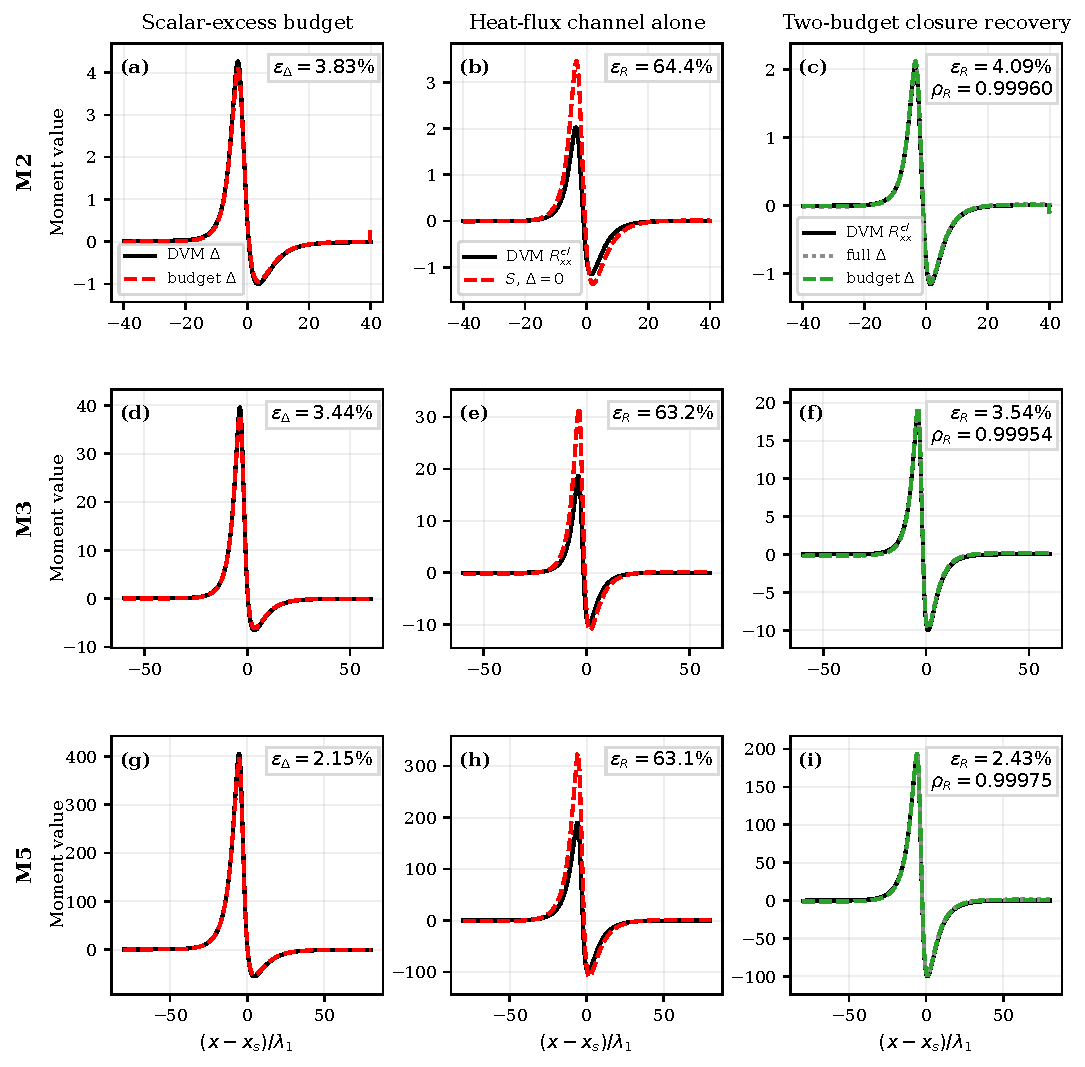
\includegraphics[width=0.99\linewidth]{figures/fig3_two_budget_recovery.pdf}}
  \caption{Two-budget recovery of the tensorial fourth-order closure moment. First column: scalar-excess budget reconstruction of $\Delta$. Second column: heat-flux channel alone, where $R^{\cl}_{xx}\simeq S$ corresponds to setting $\Delta=0$. Third column: two-budget reconstruction $R^{\cl}_{xx}\simeq S_{\rm bud}-\Delta_{\rm bud}/3$. The dotted curve shows the full-$\Delta$ reference reconstruction, i.e. the reference reconstruction obtained when the complete DVM scalar-excess field is available.}
  \label{fig:two_budget}
\end{figure}

\begin{table}
  \begin{center}
  \caption{Two-budget recovery of $R^{\cl}_{xx}$.  Errors are active-zone relative $L^2$ errors in percent.  The heat-flux budget alone gives $S$, while the scalar-excess budget supplies $\Delta$.}
  \label{tab:two_budget}
  \begin{tabular}{lrrrrr}
  \toprule
  Mach & $\epsilon_\Delta$ & $\epsilon_R(\Delta=0)$ & $\epsilon_R(\Delta_{\rm full})$ & $\epsilon_R(\Delta_{\rm bud})$ & $\rho_R(\Delta_{\rm bud})$\\
  \midrule
  M2 & 3.757 & 64.362 & 3.356 & 4.427 & 0.99950\\
  M3 & 3.457 & 63.225 & 3.101 & 3.735 & 0.99949\\
  M5 & 2.182 & 63.112 & 2.219 & 2.544 & 0.99974\\
  \bottomrule
  \end{tabular}
  \end{center}
\end{table}


\clearpage
\subsection{\revisionheading{Fourth-order channels at higher Mach numbers}}
\label{sec:high_mach}
\begin{revision}
The stored full BGK distributions extend the moment-level comparison to Mach 6, 8 and 12 (figure~\ref{fig:high_mach_moments}). These runs retain the constant-relaxation BGK model, $Pr=1$ and $\tau=1$, on the grids in table~\ref{tab:high_mach_grids}. Their spatial endpoints impose only incoming Maxwellian populations: $f(x_L,\boldsymbol v)=M_{d,1}$ for $v_x>0$ and $f(x_R,\boldsymbol v)=M_{d,2}$ for $v_x<0$, with the two reservoir states related by Rankine--Hugoniot conditions. Outgoing populations are determined by the interior solution. The stored distributions are single precision; their moments are re-evaluated in double precision, which reduces accumulation error but does not upgrade the precision of the underlying kinetic solution. Here $\Delta_d$ is measured relative to a Maxwellian matched on the discrete velocity grid, and $S_d=R^{\cl}_{xx}+\Delta_d/3$. No far-field plateau is subtracted. Increasing the matching iteration count from four to twelve changes $\Delta_d$ by at most $4.71\times10^{-6}$ in relative $L_2$ norm across the five full/lightweight datasets.

The high-Mach integrations use first-order upwind streaming and the frozen-local-target BGK relaxation update, with $\Delta t=0.75\Delta x/v_{\max}$. Table~\ref{tab:high_mach_run_audit} reports the logged time steps and completed step counts. Runs terminate at these prescribed counts, with periodic recentering and a $10^{-30}$ positivity floor, rather than a residual-based stationary stopping criterion. The different step counts and time steps also mean that full/lightweight comparisons do not isolate temporal error.
\end{revision}

\begin{table}
\centering
\revisionbox{\begin{minipage}{0.92\textwidth}\captionsetup{width=\linewidth}
\caption{Logged high-Mach BGK run parameters and upstream reservoir quadrature checks. Time steps are rounded as in the original logs; every run reaches the stated $N_t$. The final column is the stress of the fitted upstream discrete Maxwellian, normalised by $\rho_1T_1=1$; its continuum equilibrium value is zero. It is a grid diagnostic, not physical upstream stress.}
\label{tab:high_mach_run_audit}
\centering\small
\begin{tabular}{lrrr}
\toprule
Case & $\Delta t$ & $N_t$ & $\sigma_{xx}[M_{d,1}]/(\rho_1T_1)$\\
\midrule
M6 full & $2.2846\times10^{-3}$ & 120000 & 0.04233\\
M8 full & $2.0097\times10^{-3}$ & 160000 & 0.1129\\
M12 full & $1.3397\times10^{-3}$ & 220000 & 0.8413\\
M8 lightweight & $2.3448\times10^{-3}$ & 100000 & 0.1639\\
M12 lightweight & $1.5071\times10^{-3}$ & 140000 & 0.8257\\
\bottomrule
\end{tabular}
\end{minipage}}\par
\end{table}

\begin{revision}
The upstream check exposes a limitation of these historical velocity grids. Matching density, mean velocity and scalar temperature does not enforce an isotropic pressure tensor. The narrow upstream thermal population remains at $T_1=1$ while the velocity box expands to cover the hotter downstream gas; the coarse transverse spacing then produces a nonzero equilibrium stress, reaching $0.8413\rho_1T_1$ in the full Mach-12 case. The similar defect in its lightweight partner shows why close agreement between two moment profiles can coexist with a shared quadrature error. Double-precision post-processing and discrete-equilibrium subtraction do not remove errors already introduced during kinetic evolution. The high-Mach profiles are therefore exploratory evidence about the stored moment channels, with equilibrium-quadrature and temporal limitations, rather than independently validated strong-shock solutions.

Within this scope, the higher-Mach profiles show that the scalar complement remains substantial in the stored stronger-shock distributions. The ratios $\max|\Delta_d/3|/\max|R^{\cl}_{xx}|$ are 0.714, 0.716 and 0.720 at Mach 6, 8 and 12, respectively. The positive upstream lobe and negative downstream lobe persist, while their amplitudes increase in the stored nondimensional units. Thus the additional evidence is persistence of a comparable scalar contribution at higher Mach number, rather than a new observation channel or an inferred universal Mach scaling. These peak ratios do not measure pointwise cancellation. In particular, the Mach-2--5 budget-recovery errors in table~\ref{tab:two_budget} are not extrapolated to these cases: the present extension evaluates moments directly from the distributions.

For Mach 8, full/lightweight relative $L_2$ differences in $(R^{\cl}_{xx},\Delta_d,S_d)$ are $(0.274,0.234,0.253)\%$; at Mach 12 they are $(0.230,0.272,0.253)\%$. The comparison uses the common stored $x/\lambda_1$ interval, linear interpolation and the full-profile norm as denominator, without further alignment or plateau subtraction. Table~\ref{tab:high_mach_grids} makes the differences between the paired configurations explicit. At Mach 8, the spatial and velocity point counts change at fixed domain extents. At Mach 12, both extents and point counts change; the full configuration even has a slightly larger $\Delta x$ than the lightweight one. These comparisons therefore measure combined numerical sensitivity rather than isolated convergence. A separate matched-parameter Shakhov comparison with a published Mach-8 benchmark is given in appendix~\ref{app:m8_reference}.
\end{revision}
\begin{figure}
\centering
\begingroup\setlength{\fboxsep}{6pt}
\revisionbox{\begin{minipage}{0.92\textwidth}\captionsetup{width=\linewidth}
\centering
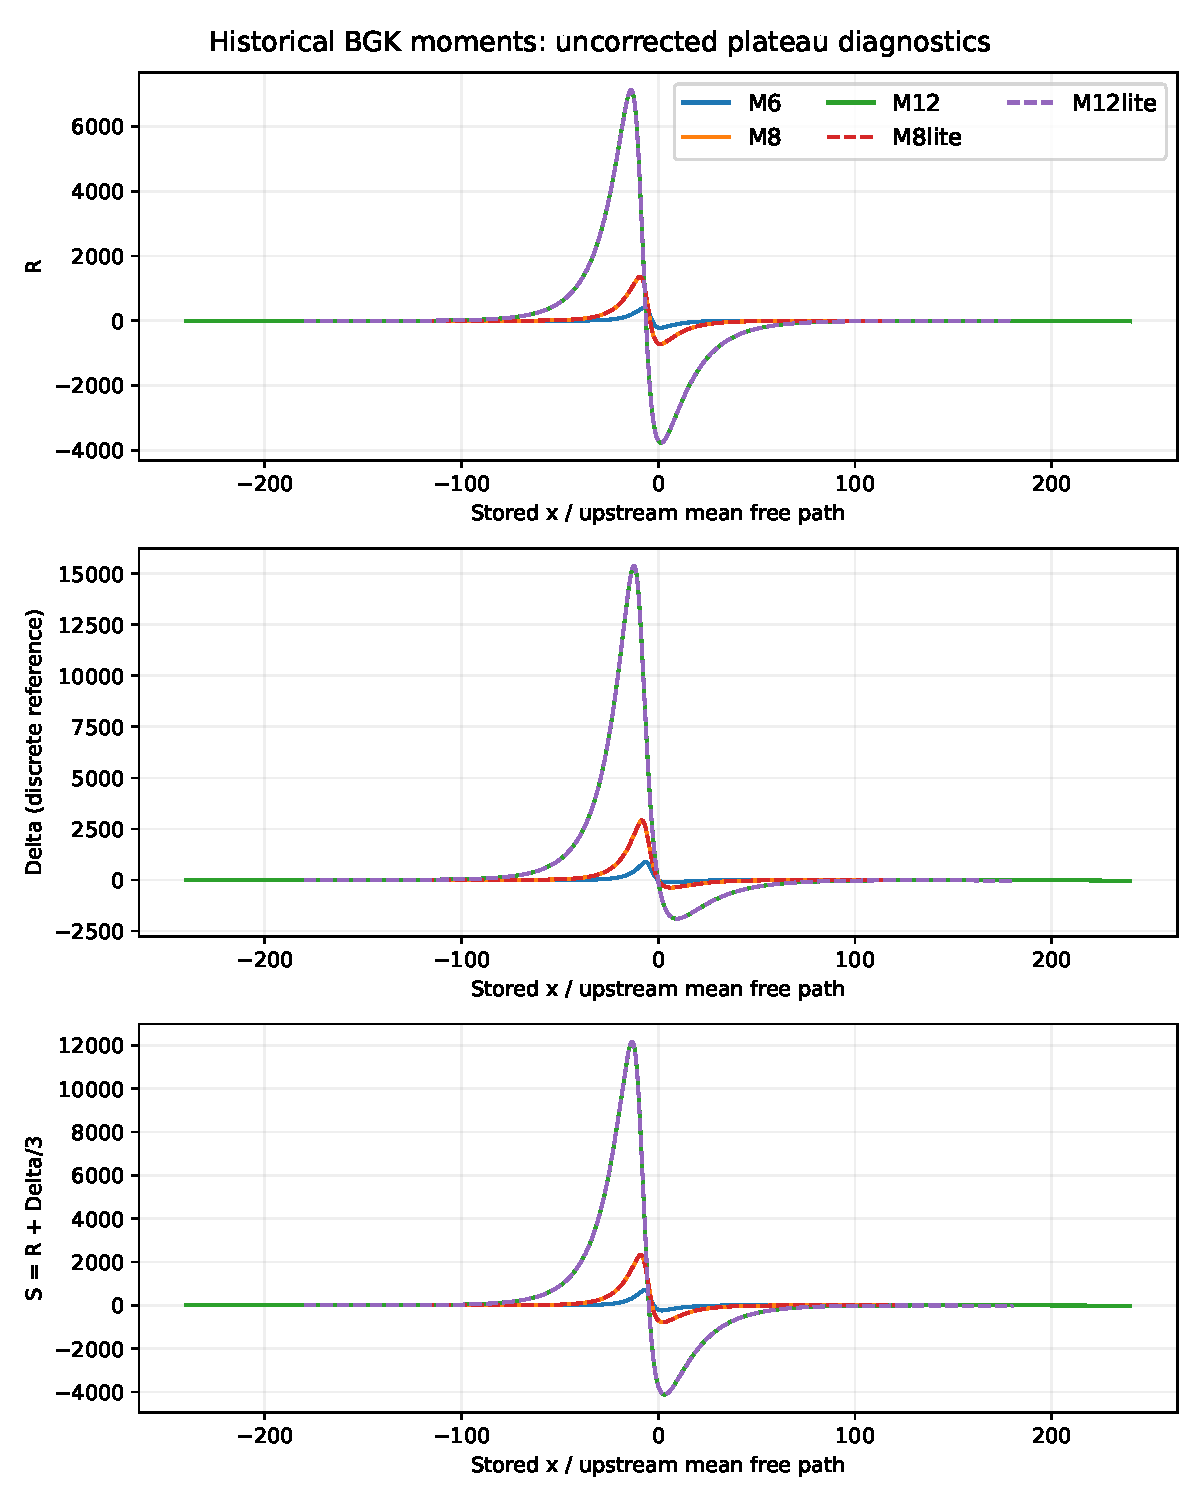
\includegraphics[width=0.98\linewidth,height=0.64\textheight,keepaspectratio]{figures/high_mach_moments.pdf}
\caption{BGK fourth-order moments at Mach 6, 8 and 12 for the full configurations in table~\ref{tab:high_mach_grids}. Dashed curves show the lightweight Mach-8 and Mach-12 variants in the same table. The discrete-reference scalar excess is retained separately from the continuum-reference excess. The plotted fields use the stored upstream mean-free-path coordinate without plateau subtraction. Full/lightweight agreement measures combined numerical sensitivity and does not establish independent velocity-tail, spatial-grid or temporal convergence; the upstream equilibrium-quadrature defects are reported in table~\ref{tab:high_mach_run_audit}.}
\label{fig:high_mach_moments}
\end{minipage}}\endgroup
\end{figure}

\clearpage
\section{Sparse scalar-excess information}
\label{sec:sparse_delta}

The budget reconstruction above uses full DVM moments to establish the physical channel.  To test whether this channel represents reduced information rather than disguised direct access to $R^{\cl}_{xx}$, we replace the full $\Delta$ field by a sparse scalar-excess probe.  The DVM $\Delta$ profile is sampled at 24 shock-local interior points with two endpoint anchors and reconstructed with a smooth radial-basis-function (RBF) representation; no values of $R^{\cl}_{xx}$ are used.  The tensorial closure is then computed from $R^{\cl}_{xx}=S-\Delta_{\rm sparse}/3$.

\begin{revision}
Figure~\ref{fig:sparse_delta} reports a separate interpolation test using its archived, fixed heat-budget channel. With 24 shock-local interior samples of $\Delta$ and two endpoint anchors, the tensorial errors are $4.33\%$, $4.49\%$ and $3.77\%$ for $M_1=2,3,5$; adding $1\%$ probe noise keeps the error below $4.7\%$ under that same contract. These results test scalar information reduction within the archived channel; they are not a new sparse-probe evaluation of the regenerated discrete-source budget in table~\ref{tab:two_budget}. The full-field reference curves in this interpolation study belong to the same archived contract.
\end{revision}

\begin{revision}
This is an interpolation and information-reduction experiment, not a theorem that 24 probes are sufficient in a universal or optimal sense.  
\end{revision}

\begin{revision}
The structural statement is instead that the missing information has the type of one scalar fourth-order field; the number of probes required to interpolate that field depends on smoothness, shock thickness, noise level and probe placement.  The convergence curve in figure~\ref{fig:sparse_delta}(a) should therefore be read as an operating study for the present shock family.  Small numbers of probes already remove the order-unity ambiguity, and the 24-interior-probe case is a tested operating point within the fixed-channel interpolation experiment, not a certified sensor minimum or a comparison with the newly regenerated full-field budget.  Thus the information needed to resolve the heat-flux ambiguity is not a dense $R^{\cl}_{xx}$ field; it is an independent scalar measure of isotropic fourth-order tail intensity.  This distinction matters for experiments and reduced solvers: a scalar diagnostic, surrogate or auxiliary equation for tail intensity can close the heat-flux null space without supervising the whole tensorial closure field.
\end{revision}

\begin{figure}
  \centerline{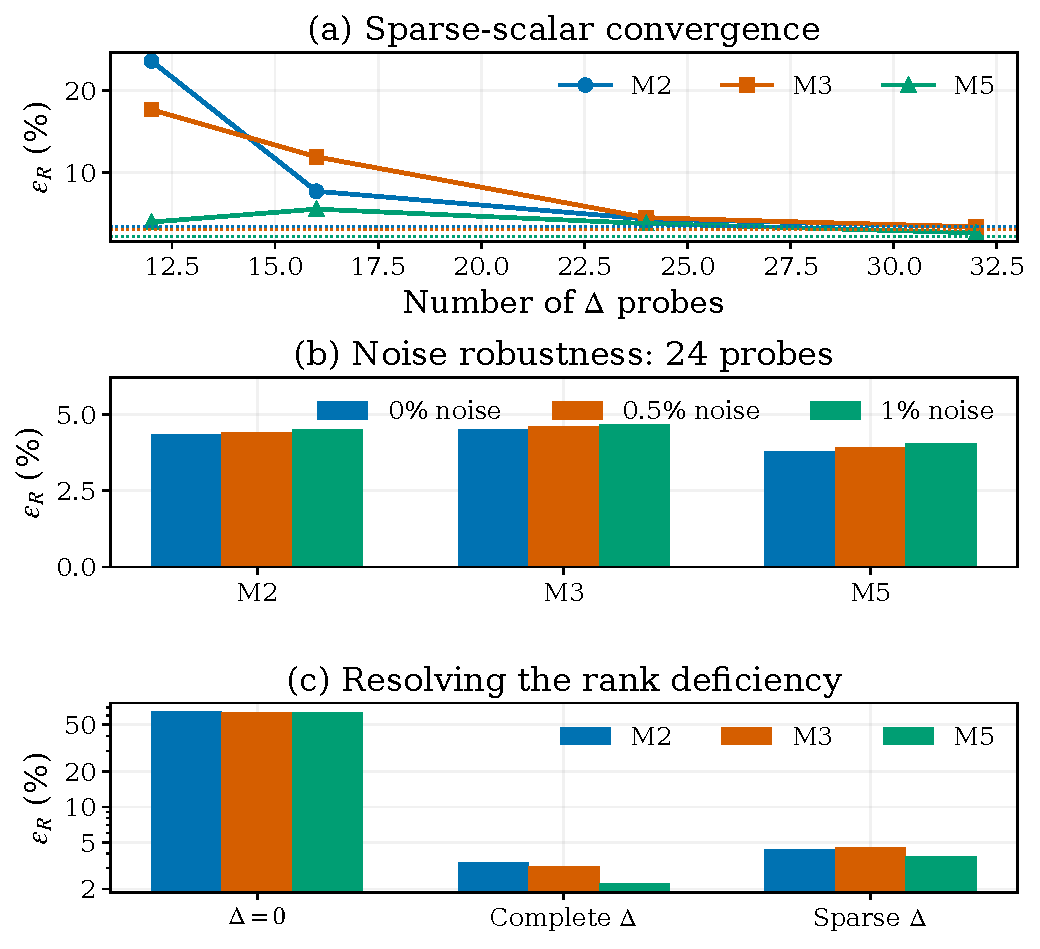
\includegraphics[width=0.96\linewidth]{figures/fig4_sparse_delta_robustness.pdf}}
  \caption{Sparse scalar-excess information tested with the archived fixed heat-budget channel, separate from the regenerated budget in table~\ref{tab:two_budget}. (a) Convergence of the $R^{\cl}_{xx}$ reconstruction error as the number of shock-local $\Delta$ probes increases; dotted lines denote the full-$\Delta$ reference errors and the 24-interior-probe case, supplemented by two endpoint anchors, is a representative operating point for this interpolation test in (b,c). (b) Robustness of the 24-probe reconstruction to $0.5\%$ and $1\%$ noise in the $\Delta$ probes. (c) Comparison between the rank-deficient heat-flux reconstruction $(\Delta=0)$, the full-$\Delta$ reference reconstruction and the 24-probe sparse-$\Delta$ reconstruction.}
  \label{fig:sparse_delta}
\end{figure}


\begin{revision}
\textbf{Sensitivity to probe placement.} The small errors above apply to the specified shock-local sampling layouts, not arbitrary sets of 24 points. Figure~\ref{fig:revision_sparse_gap} tests this distinction on the completed Mach-5 baseline. With the same 24 interior probes and two boundary anchors, an active-uniform layout gives a $3.107\%$ active-zone error in $R^{\cl}_{xx}$, whereas a gap of width $25\%$ of the active interval, centred at the largest scalar-excess magnitude, raises that error to $33.014\%$. The existing full-domain-uniform layout, with 24 total probes including endpoints, gives $17.385\%$ and is not an exactly equal-count comparison. These controlled tests supply $S=R^{\cl}_{xx}+\Delta/3$ exactly to isolate scalar interpolation error; they do not revalidate the budget-derived channel or replace the earlier Mach-sweep errors. The active interval is chosen using the reference field, so the experiment also does not demonstrate blind sensor placement. A low leave-one-out error on observed probes does not guarantee accuracy within an unobserved core gap. The practical sparse-recovery claim therefore requires adequate core coverage.
\end{revision}

\begin{figure}
\centering
\begingroup\setlength{\fboxsep}{6pt}
\revisionbox{\begin{minipage}{0.92\textwidth}\captionsetup{width=\linewidth}
\centering
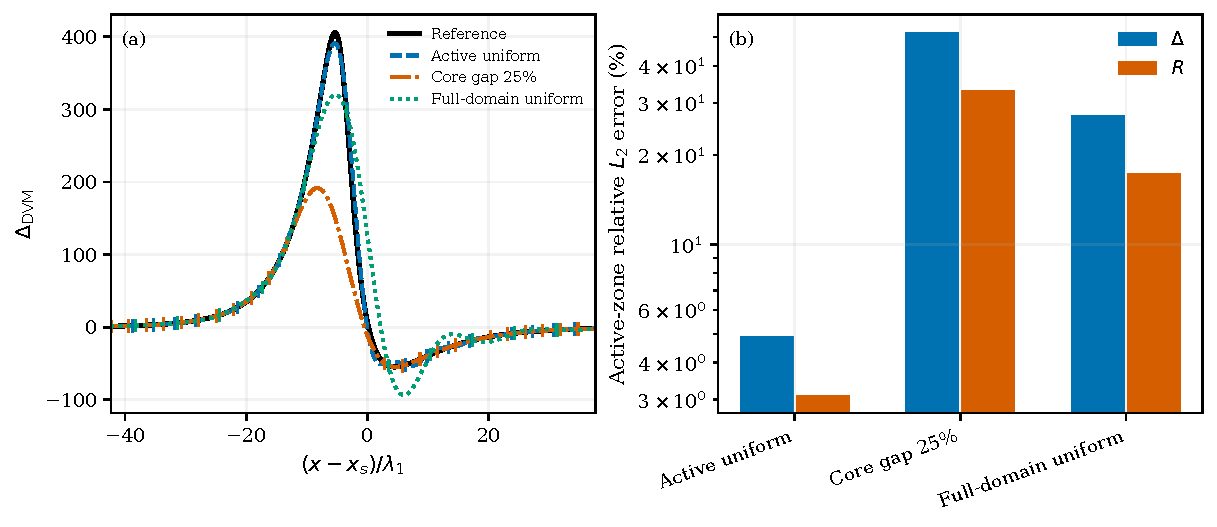
\includegraphics[width=\linewidth]{figures/A4_sparse_core_gap.pdf}
\caption{Controlled probe-placement sensitivity for the Mach-5 scalar channel. Left: reference and Gaussian RBF reconstructions, with probe locations marked. Right: relative $L_2$ errors over $|\Delta|\geq0.02\max|\Delta|$. Active-uniform and core-gap layouts have 26 total probes (16 and 14 in the active interval); full-domain uniform has 24 total (seven active). The active span is padded by $25\%$ on either side; the gap width is $25\%$ of the unpadded active span. The mean of the outermost $8\%$ at each end is subtracted following the existing interpolation procedure. Gaussian-RBF parameters are selected from sparse data by leave-one-out validation: 28/32/48 centres, width multipliers 0.5/0.6/0.8/1/1.2/1.5 and ridge parameters $10^{-10}/10^{-8}/10^{-6}/10^{-4}/10^{-2}$. No noise is added; $S$ is exact. This is a controlled interpolation stress test, not full two-budget validation.}
\label{fig:revision_sparse_gap}
\end{minipage}}
\endgroup
\end{figure}

\section{Direct DSMC collision production of the scalar-excess source}
\label{sec:dsmc}

The relaxation models above are useful because they isolate specific collision-model mechanisms.  BGK and Shakhov relax the scalar excess as $-\Delta/\Kn$, while ES-BGK adds a stress-quadratic target contribution.  A stronger test is to measure the scalar-excess production from collisions without prescribing any relaxation target.  We therefore perform a standalone DSMC calculation of a Mach-3 monatomic hard-sphere normal shock and accumulate the production of the central fourth scalar moment directly during accepted binary collisions.

For each accepted collision pair in cell $j$, let $\boldsymbol c_1$ and $\boldsymbol c_2$ denote peculiar velocities relative to the instantaneous cell mean velocity before collision, and let primed quantities denote the post-collision velocities after elastic hard-sphere scattering.  The cell-wise scalar-excess production is sampled as
\begin{equation}
  Q_{\Delta,j}^{\rm DSMC}
  =\frac{1}{V_j\Delta t_{\rm samp}}
  \sum_{\rm coll\in j}
  \left[
  |\boldsymbol c'_1|^4+|\boldsymbol c'_2|^4
  -|\boldsymbol c_1|^4-|\boldsymbol c_2|^4
  \right]w_p,
  \label{eq:dsmc_qdelta}
\end{equation}
Here $j$ labels a collision cell of volume $V_j$, and the sum runs
over accepted binary collisions accumulated during the exposure
$\Delta t_{\rm samp}$. The constant weight $w_p$ is the mass
represented by one simulation particle (equivalently molecular count
in unit molecular-mass units). Pair labels 1 and 2 denote the two
particles, using the same pre-collision cell mean $\boldsymbol u_j$:
$\boldsymbol c_\ell=\boldsymbol v_\ell-\boldsymbol u_j$ and
$\boldsymbol c'_\ell=\boldsymbol v'_\ell-\boldsymbol u_j$.
Primes here denote post-collision values, whereas $u_x'$ denotes a
spatial derivative. The exposure is the time represented by accumulated
collision events, rather than the spacing between stored moment samples.
$Q(f,f)$ is the Boltzmann binary-collision operator.  This quantity is the DSMC counterpart of $\int |\boldsymbol c|^4Q(f,f)\,\dd\boldsymbol v$.  It is not imposed to be proportional to $-\Delta$; it is a direct measurement of how binary collisions create or destroy the scalar-excess moment in the shock layer.

For this hard-sphere campaign,
$\lambda_1=(\sqrt{2}\,n_1\Sigma_T)^{-1}$ is the upstream mean free
path, where $n_1$ is molecular number density and $\Sigma_T$ the total
hard-sphere cross-section. PPC denotes the nominal upstream
simulation-particle count per spatial cell; independent seeds denote
independent pseudorandom initialisations. The DSMC run uses 400 spatial cells over $[-60,60]\lambda_1$, upstream particles per cell equal to 120, time step $0.005$, and eight independent seeds.  Sampling starts after 70000 steps and continues to 180000 steps, with sampling every 10 steps.  The realisations are aligned by their density-midpoint shock locations before averaging.  Each realisation has 11001 stored moment samples and an average of $8.2\times10^5$ accepted collisions per active-zone cell.  This alignment is essential: the scalar-excess budget contains the derivative of the fifth-order flux $J_\Delta$, and direct averaging of unaligned shock profiles smears the derivative even when the lower-order shock structure appears converged.

\begin{revision}
Figure~\ref{fig:dsmc_budget} shows the result.  Panel (a) verifies that the direct DSMC calculation samples the same nonequilibrium shock layer in which the heat flux and normal stress are concentrated.  Panel (b) shows the scalar excess $\Delta$.  Panel (c) compares the directly accumulated collisional production $Q_\Delta^{\rm DSMC}$ with the spatial scalar-excess budget,
\begin{equation}
  Q_\Delta^{\rm budget}=\partial_xJ_\Delta+4(\partial_xu_x)K_\Delta .
  \label{eq:dsmc_budget}
\end{equation}
The derivative is evaluated using a local cubic polynomial with a seven-point stencil; windows of 5--9 points give similar results, while larger windows over-smooth the narrow shock layer.  Specifically, stencil windows of 5, 7 and 9 give active-zone errors $0.173$, $0.170$ and $0.188$, and correlations $0.986$, $0.987$ and $0.984$, respectively.  The active-zone comparison reported in figure~\ref{fig:dsmc_budget} gives a relative error of 0.170 and a correlation of 0.987.  For DSMC, both sides of \eqref{eq:dsmc_budget} are difficult quantities: one is a noisy collision-production sample and the other contains a derivative of a fifth-order flux.  The comparison supports the collision-production interpretation of the scalar-excess channel within the tested implementation; the sampler audit below limits its use as a validation of the Boltzmann operator.
\end{revision}

Panel (d) compares the normalised collision production with the normalised $-\Delta$ profile.  The correlation is 0.968, showing that the DSMC collisions relax the scalar excess in the shock core with the same qualitative sign structure as BGK and Shakhov.  The comparison is deliberately normalised: the DSMC production is not assumed to follow the BGK/Shakhov unit relaxation rate, and the effective proportionality varies through the shock.  This is precisely the point.  The scalar channel identified by the two-budget theory is not a relaxation-model artefact; it is a collisional channel whose source law becomes model-dependent once one moves from BGK to Shakhov, ES-BGK, ES-FP and DSMC/Boltzmann physics.

\begin{figure}
  \centerline{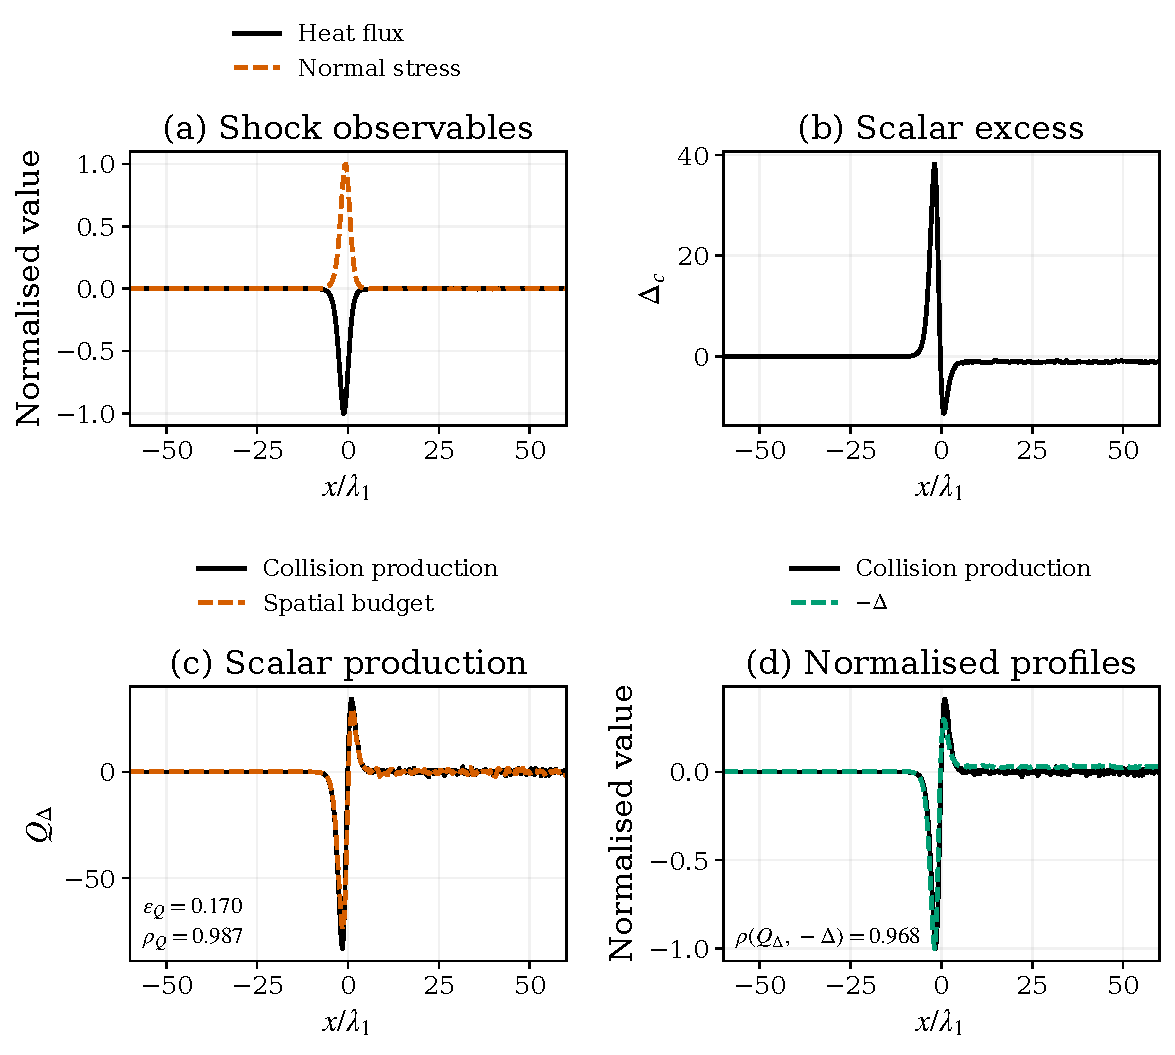
\includegraphics[width=0.95\linewidth]{figures/fig6_dsmc_delta_budget.pdf}}
  \caption{Direct DSMC scalar-excess production in a Mach-3 monatomic hard-sphere shock.  (a) Normalised heat flux and normal stress identify the nonequilibrium shock layer.  (b) Scalar fourth-order excess $\Delta$.  (c) Direct collisional production $Q_\Delta^{\rm DSMC}$, accumulated from pre- and post-collision changes of $|\boldsymbol c|^4$, compared with the spatial budget $\partial_xJ_\Delta+4u_x'K_\Delta$.  Realisations are aligned at their density midpoints before averaging; the plotted $x/\lambda_1$ is this aligned coordinate, $(x-x_s)/\lambda_1$. The active-zone relative error is 0.170 and the correlation is 0.987.  (d) Normalised $Q_\Delta^{\rm DSMC}$ and $-\Delta$ have correlation 0.968, indicating strong relaxation-like alignment without assuming a BGK relaxation rate.}
  \label{fig:dsmc_budget}
\end{figure}

\begin{revision}
The DSMC calculation extends the source diagnostics to directly sampled binary collisions. Together with the model sources in table~\ref{tab:source_laws}, it illustrates how a common heat-flux observation channel can coexist with different scalar-production laws. The pair-selection limitation discussed in the sampler audit below applies to the quantitative DSMC comparisons.
\end{revision}


\begin{revision}
\textbf{Particle-number audit and interpretation.} The original ensemble with 120 particles per cell (PPC120) is supplemented by PPC60, 240, 480, 960, 1920 and 3840, each with eight seeds and the same grid, time step and sampling schedule, giving 56 runs. Figure~\ref{fig:revision_dsmc_moments} shows the high-PPC moment profiles; appendix~\ref{app:particle_sensitivity} reports the directly logged collision-source audit. Between PPC1920 and PPC3840, aligned ensemble-mean $R^{\cl}_{xx}$, $\Delta$ and $S$ differences are approximately $0.385\%$, $0.391\%$ and $0.309\%$, and the collision-source difference is $0.668\%$. These finite-sample differences do not establish statistical equivalence or independence from the sampling window. 

Moreover, an audit identified a pair-selection bias in the original DSMC sampler; corrected-sampler pilots are separate and have not been mixed into this ensemble. Consequently, the original-source budget correlations remain diagnostics of that implementation, not a bias-free validation of the Boltzmann collision operator. Between-seed intervals do not account for this systematic error.
\end{revision}

\begin{figure}
\centering
\begingroup\setlength{\fboxsep}{6pt}
\revisionbox{\begin{minipage}{0.92\textwidth}\captionsetup{width=\linewidth}
\centering
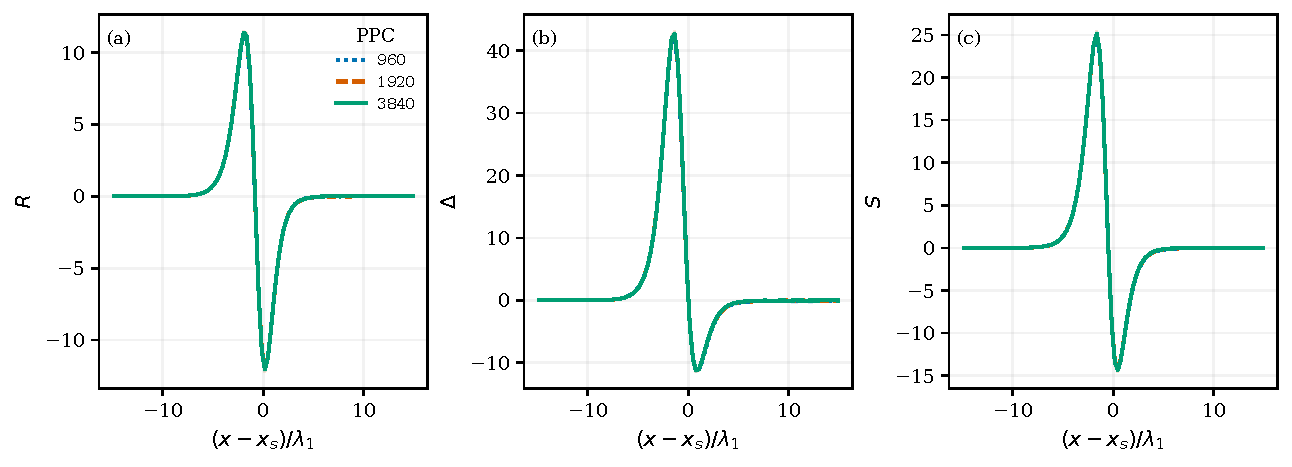
\includegraphics[width=\linewidth]{figures/Main_DSMC_high_moments.pdf}
\caption{Mach-3 hard-sphere DSMC high-order moments at PPC960, 1920 and 3840. Lines show eight-seed means and bands pointwise $95\%$ Student-$t$ intervals with seven degrees of freedom. Each time-averaged profile is aligned at its $n=2$ crossing by linear interpolation, without smoothing; $\lambda_1=1$ in the DSMC units. The bands exclude systematic sampler error and are not simultaneous confidence bands. These are original-sampler results; the identified pair-selection bias remains unresolved. Alignment does not remove temporal shock wandering. The Mach-3 DSMC fields are not a direct same-case validation of the Mach-5 DVM comparisons.}
\label{fig:revision_dsmc_moments}
\end{minipage}}
\endgroup
\end{figure}

\section{Consequences and outlook for closure modelling}
\label{sec:consequences}

The identifiability result has a direct consequence for closure modelling.  If a model is trained, fitted or regularised only through the heat-flux budget, then all states related by \eqref{eq:null_transform} are observationally equivalent to that budget.  A one-parameter family
\begin{equation}
  R^{\cl}_{xx,\eta}=R^{\cl}_{xx}+\eta(x),\qquad
  \Delta_{\eta}=\Delta-3\eta(x)
  \label{eq:closure_family}
\end{equation}
produces exactly the same observed channel $S$ for any shock-local field $\eta(x)$.  Two closures can therefore agree in the heat-flux residual and disagree in the tensorial closure moment required by an R26-type model.  This is not merely a diagnostic inconvenience.  The tensorial and scalar parts enter different members of a moment hierarchy and represent different pieces of the nonequilibrium distribution: traceless anisotropy and isotropic tail intensity.  Treating their sum as the tensorial moment itself can therefore produce a closure with the correct observed energy-transport channel and the wrong internal split.  In R26 language, such a closure would appear successful when inspected through the heat-flux equation, but it would supply the wrong tensorial fourth-order state to any equation, wall condition or regularisation term that depends on $R^{\cl}_{ij}$ rather than on the composite $A_{ij}=R^{\cl}_{ij}+\Delta\delta_{ij}/3$.

\begin{revision}
These shocks provide a reference test for reduced kinetic solvers, neural closures and moment models: recover $S$, supply independent scalar-excess information, and then infer $R^{\cl}_{xx}$. Agreement in low-order profiles alone cannot test this split. The sparse-probe results show that the scalar information can be sampled at a limited number of locations when those locations adequately cover the shock core.
\end{revision}

\begin{revision}
The ES-BGK and ES-FP diagnostics (table~\ref{tab:model_source_corrections} and figure~\ref{fig:esfp_esbgk_sources}) modify scalar production through stress anisotropy while retaining the heat-flux observation channel. Independently evolved ES-BGK Mach-2/3 fields are reported in appendix~\ref{app:esbgk_evolved}; these finite-time calculations preserve positive states but have not passed the specified stationarity criterion. On the same DVM profiles, ES-FP gives the larger correction. Figure~\ref{fig:dsmc_budget} adds the binary-collision diagnostic, subject to the original-sampler bias in \S\ref{sec:dsmc}. Thus testing the observation map and testing the collision-source law remain separate requirements.
\end{revision}

\begin{revision}
In multidimensional flows, the observed heat-flux quantity is the divergence of the composite tensor $R^{\cl}_{ij}+\Delta\delta_{ij}/3$, so additional tensorial information is needed to reconstruct the full closure tensor.  The one-dimensional shock studied here is therefore the clean base problem, not the end point of the theory.
\end{revision}


\begin{revision}
\textbf{Relation to realizability and closed-system stability.} The family in the displayed null-space family describes an unobserved direction in one balance law, not a family of admissible solutions of a closed R26 system. A residual that observes only $S$ does not penalise changes along that direction or test their moment realizability. The scalar complement removes this observational freedom; positivity and realizability constraints must still be imposed independently. Hyperbolicity additionally depends on the constitutive flux laws for $m_{ijk}$, $R^{\cl}_{ij}$ and $\Delta$. No closed-system principal symbol is evaluated here, so removing the null direction does not prove a real spectrum, removal of the Bobylev instability or hypoellipticity. In multiple dimensions, complementary observations would need to resolve the irreducible rotational components, for example in a representation of the Lie algebra $\mathfrak{so}(3)$ of three-dimensional rotations, rather than append only one scalar observation.

The two-budget procedure is primarily an identifiability diagnostic. It is constructive when an invertible scalar source law, the required fluxes and an anchor are supplied, as for these BGK references. For general Boltzmann production, a measured source does not alone determine $\Delta$ algebraically.

\textbf{Scope of the channel result.} Invertibility of the two-observation map does not imply positivity of an underlying distribution, hyperbolicity of a closed moment system, or an entropy inequality. No closed flux Jacobian is constructed here, and no restoration of a real spectrum or hypoellipticity is claimed. In multiple dimensions, observing a tensor divergence does not identify all tensor components: adding a scalar channel is not generally sufficient. The present reservoir-boundary shock calculation supplies no solid-wall moment boundary law. Polyatomic internal energies would enlarge the moment state and introduce additional exchange channels; the one-dimensional monatomic rank calculation cannot be transferred unchanged. Finally, this work does not train a constitutive closure or establish its Chapman--Enskog limit. Varying a mean-free-path coordinate alone is not an independent macroscopic hydrodynamic-limit test. The reported $2.54$--$4.43\%$ recovery range concerns the tested BGK references, not arbitrary molecular cross-sections.
\end{revision}

\section{Conclusions}
\label{sec:conclusion}

The heat-flux budget of a monatomic kinetic normal shock constrains a combined fourth-order energy-transport channel, not the tensorial closure moment alone.  In one dimension this channel is $S=R^{\cl}_{xx}+\Delta/3$, and the observation map from $(R^{\cl}_{xx},\Delta)$ to $S$ has a one-dimensional null space.  This projection property explains why residual agreement in the heat-flux equation cannot by itself certify recovery of every R26-level closure variable.

\begin{revision}
The missing scalar channel can be supplied constructively.  A DVM-consistent scalar-excess budget supplies the missing scalar field, and the two budgets recover $R^{\cl}_{xx}$ without direct $R$ data.  For the tested $Pr=1$ BGK shocks at Mach 2, 3 and 5, the error falls from about $63$--$64\%$ to $2.54$--$4.43\%$.  With adequate shock-core coverage, sparse scalar-excess probes approach the full-field recovery accuracy in the tested shocks. The missing information is one scalar channel; the number and placement of probes needed to reconstruct it depend on the shock profile. These errors do not include a Mach-4 budget test or the separate $Pr=2/3$ cross-method campaign.
\end{revision}

\begin{revision}
The collision-model analysis shows that the observation channel and the source law must be kept separate.  Table~\ref{tab:source_laws} summarises the ladder.  Shakhov corrects the heat-flux relaxation to $Pr=2/3$ while leaving the even scalar-excess source invariant.  ES-BGK leaves the heat-flux observation channel unchanged but modifies the scalar-excess source through a stress-quadratic anisotropic-Gaussian target, contributing about $4.3$--$4.5\%$ of $\|\Delta\|$ in the present Mach 2--5 profiles.  ES-FP gives a larger anisotropic-diffusion correction of about $21.5$--$22.4\%$ while remaining strongly correlated with the BGK/Shakhov source.  Finally, DSMC measures the corresponding fourth-order production directly from accepted binary collisions.  In the original-sampler Mach-3 DSMC ensemble, the direct collisional production and spatial scalar-excess budget have correlation 0.987, while the production and $-\Delta$ have correlation 0.968. The identified pair-selection bias limits both comparisons to diagnostics of that implementation.  Thus the scalar-excess channel is not an artefact of BGK-type relaxation targets; it is a physical collision-production channel whose specific source law changes as one moves from BGK and Shakhov to ES-BGK, ES-FP and Boltzmann/DSMC.
\end{revision}

\begin{revision}
The higher-Mach BGK distributions extend the direct moment comparison to Mach 6, 8 and 12 on the case-dependent spatial and velocity domains in table~\ref{tab:high_mach_grids}. Their peak scalar-to-tensorial ratios $\max|\Delta_d/3|/\max|R^{\cl}_{xx}|$ are 0.714, 0.716 and 0.720, respectively. The scalar complement remains substantial in these stored distributions, subject to the equilibrium-quadrature defects in table~\ref{tab:high_mach_run_audit}. Full/lightweight profile differences of roughly $0.23$--$0.27\%$ at Mach 8 and 12 measure combined numerical sensitivity; they do not extend the Mach-2--5 budget-recovery result or establish isolated convergence. The separate Mach-8 Shakhov comparison in appendix~\ref{app:m8_reference} tests density and temperature against published profiles, with stationarity and positivity limitations explicitly retained.
\end{revision}


\begin{revision}
The numerical evidence must be distinguished from the identifiability statement. The observation-map null space is an algebraic property; small discretisation sensitivities do not prove hyperbolicity, entropy stability or convergence of every collision model. The sparse-recovery operating point requires shock-core coverage, and the corrected-sampler comparison quantifies rather than eliminates uncertainty associated with pair selection. The final velocity-grid comparison is complete. At PPC 960, the eight-seed differences in the three moment profiles are below $1\%$, while the collision-source difference is $1.413\%$; these differences are comparable to the estimated sampling uncertainty. Neither this comparison nor the entropy diagnostic establishes universal model validation (appendix~\ref{app:additional_audits}).
\end{revision}

\begin{revision}
As a separate profile-level benchmark, appendix~\ref{app:dsmc_cross_method} compares high-particle-count Bird DSMC shocks at Mach 2--5 with available Shakhov DVM snapshots and corrected-Shakhov R26 profiles. This comparison complements, but does not replace, the DSMC collision-production and sampler-sensitivity studies: the new runs contain one seed per Mach and do not record the collision-wise $Q_\Delta$ observable used in \S\ref{sec:dsmc}.
\end{revision}

\section*{Funding}
This research received no specific grant from any funding agency, commercial or not-for-profit sectors.

\section*{Declaration of AI-assisted tools}
ChatGPT (OpenAI) and Claude (Anthropic) assisted with language editing, numerical-script debugging and critical review of the manuscript and response letters. The author is responsible for verifying the numerical results, figures, equations, references and scientific conclusions; AI suggestions were not treated as independent scientific evidence.

\section*{Declaration of interests}
The author reports no conflict of interest.

\section*{Data availability statement}
\begingroup\raggedright
Manuscript sources, figure and table files, recoverable solver and analysis source snapshots, compact numerical profiles and run/check records are deposited in the public repository \url{https://github.com/Ehsan-Roohi/DVM-JFM}; the scientific deposit is identified by commit \texttt{4c3d311}, and the accompanying reader-facing revision is identified by tag \texttt{reviewer-revision-20261010} \citep{RoohiShockArchive2026}. The independent ES-BGK Mach-2/3 deposit, including all six completed $t=400$ reduced-distribution checkpoints, budget arrays, profiles and reproducible comparison scripts, is identified separately by tag \texttt{esbgk-m2-m3-t400-20261011}. Its own deposit manifest records file sizes and SHA-256 hashes. Continuations are kept outside this frozen finite-time deposit. The original publication manifest records file sizes and SHA-256 hashes, while its solver-specification and coverage audits distinguish the collision-model campaigns, historical and corrected calculations, and unresolved provenance gaps. The bundled Mach-2 and Mach-3 raw-profile comparison scripts reproduce the deposited comparison tables. This deposit does not contain all multi-gigabyte velocity-distribution/restart files, and some archived drivers require adaptation of machine-specific paths. The Bird DSMC original remains an external dependency; the repository supplies the documented modifications and original-source identification. The archived budgets have been regenerated with their documented discrete-source contracts. The full distribution used for Figure~\ref{fig:shakhov_check} is included in the public repository with its hash; a complete public deposit of the larger BGK raw distributions remains outstanding. No DOI has yet been assigned.\par\endgroup


\clearpage
\appendix
\section{\revisionheading{DVM numerical sensitivity}}
\label{app:numerical_sensitivity}

\begin{revision}
This appendix concerns the Mach-5 BGK sensitivity campaign. 
The velocity integrals use uniform tensor-product composite-trapezoidal weights, including half endpoint weights on each axis. Streaming is advanced explicitly with first-order upwind differences and $\Delta t=C_{\rm CFL}\Delta x/v_{\max}$. A local discrete Maxwellian is formed by iteratively matching density, streamwise velocity and temperature, followed by the frozen-local-target update $f^{n+1}=M+(f^*-M)\exp(-\Delta t)$. 

The code uses unit relaxation rate in these computational coordinates; a macroscopic-length definition of $\Kn$ must not be inserted into these arrays without transforming the transport and source scales together. Maxwellian reservoirs supply incoming velocities at the left and right boundaries, at Rankine--Hugoniot states. There are no solid walls. 

The implementation recentres the shock periodically and applies a positivity floor of $10^{-30}$. These operations are part of the numerical method, not proofs of moment-budget preservation. Runs end at the prescribed step counts; the reported late-profile changes diagnose stationarity but are not an implemented residual-based stopping test. Conservation of low-order moments by the fitted Maxwellian does not guarantee exact equilibrium values of higher moments on a finite velocity grid.
For each field $g\in\{\rho,T,q_x,R^{\cl}_{xx},\Delta_d,S\}$, the comparison uses $100\|g_{\rm base}-g_{\rm test}\|_2/\|g_{\rm test}\|_2$ on 601 equally spaced points in $|(x-x_s)/\lambda_1|\leq15$. Each profile is independently aligned at its density midpoint and linearly interpolated without additional smoothing or plateau correction. The test profile is the denominator, not an exact reference solution. 

The baseline has $N_x=2200$, half-domain $80\lambda_1$, velocity grid $141\times27\times27$ and $v_{\max}=22$. The enlarged velocity domain uses $169\times33\times33$ points with longitudinal bound 26.4 and transverse bound 27.076923. Velocity refinement uses $211\times40\times40$ points at the baseline extent. Spatial refinement uses 3299 points; the enlarged spatial half-domain is $120\lambda_1$ with 3300 points. The time-step test halves the baseline CFL coefficient from 0.75 to 0.375. Prescribed step counts for baseline, velocity extent, velocity refinement, spatial refinement, half time step and spatial extent are 52000, 62400, 52000, 78000, 104000 and 52000, respectively. All six integrations reached their prescribed end steps; final profiles, matching checkpoints and archive checksums were verified.
\end{revision}

\begin{figure}
\centering
\begingroup\setlength{\fboxsep}{6pt}
\revisionbox{\begin{minipage}{0.92\textwidth}\captionsetup{width=\linewidth}
\centering
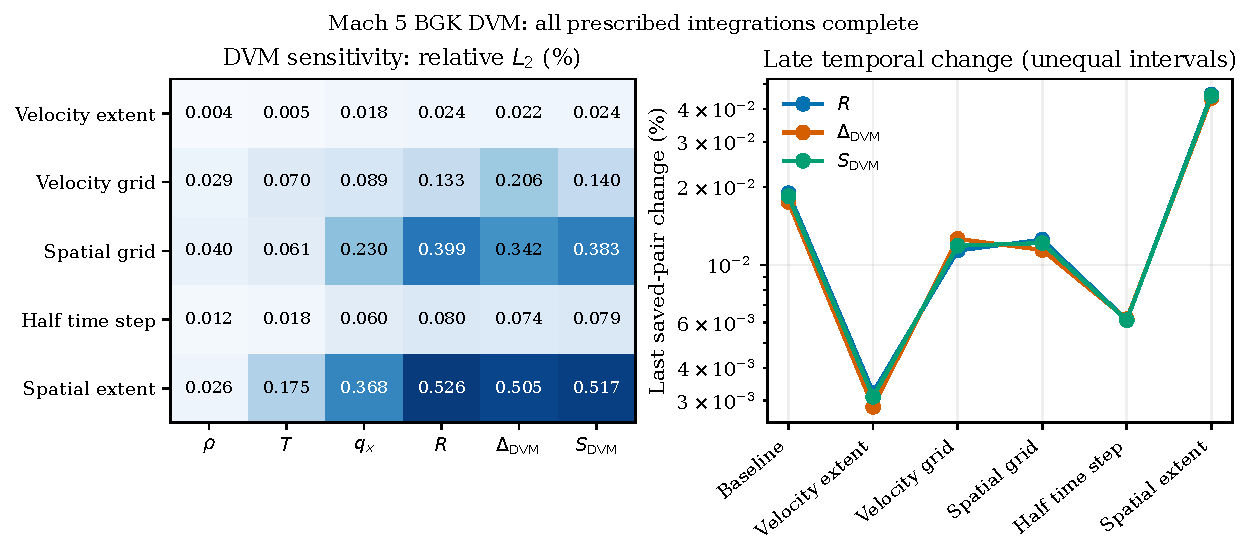
\includegraphics[width=\linewidth]{figures/A1_DVM_sensitivity_summary.pdf}
\caption{Mach-5 BGK DVM sensitivity summary. Left: relative $L_2$ differences defined in the text. Right: relative changes between the last two saved profiles, at step pairs 50000--52000, 62000--62400, 50000--52000, 76000--78000, 102000--104000 and 50000--52000 in the displayed case order. Unequal intervals are not comparable time derivatives. Two levels do not establish asymptotic convergence order; spatial refinement also changes the time step. These diagnostics introduce no new stopping threshold.}
\label{fig:revision_dvm_summary}
\end{minipage}}
\endgroup
\end{figure}

\begin{figure}
\centering
\begingroup\setlength{\fboxsep}{6pt}
\revisionbox{\begin{minipage}{0.92\textwidth}\captionsetup{width=\linewidth}
\centering
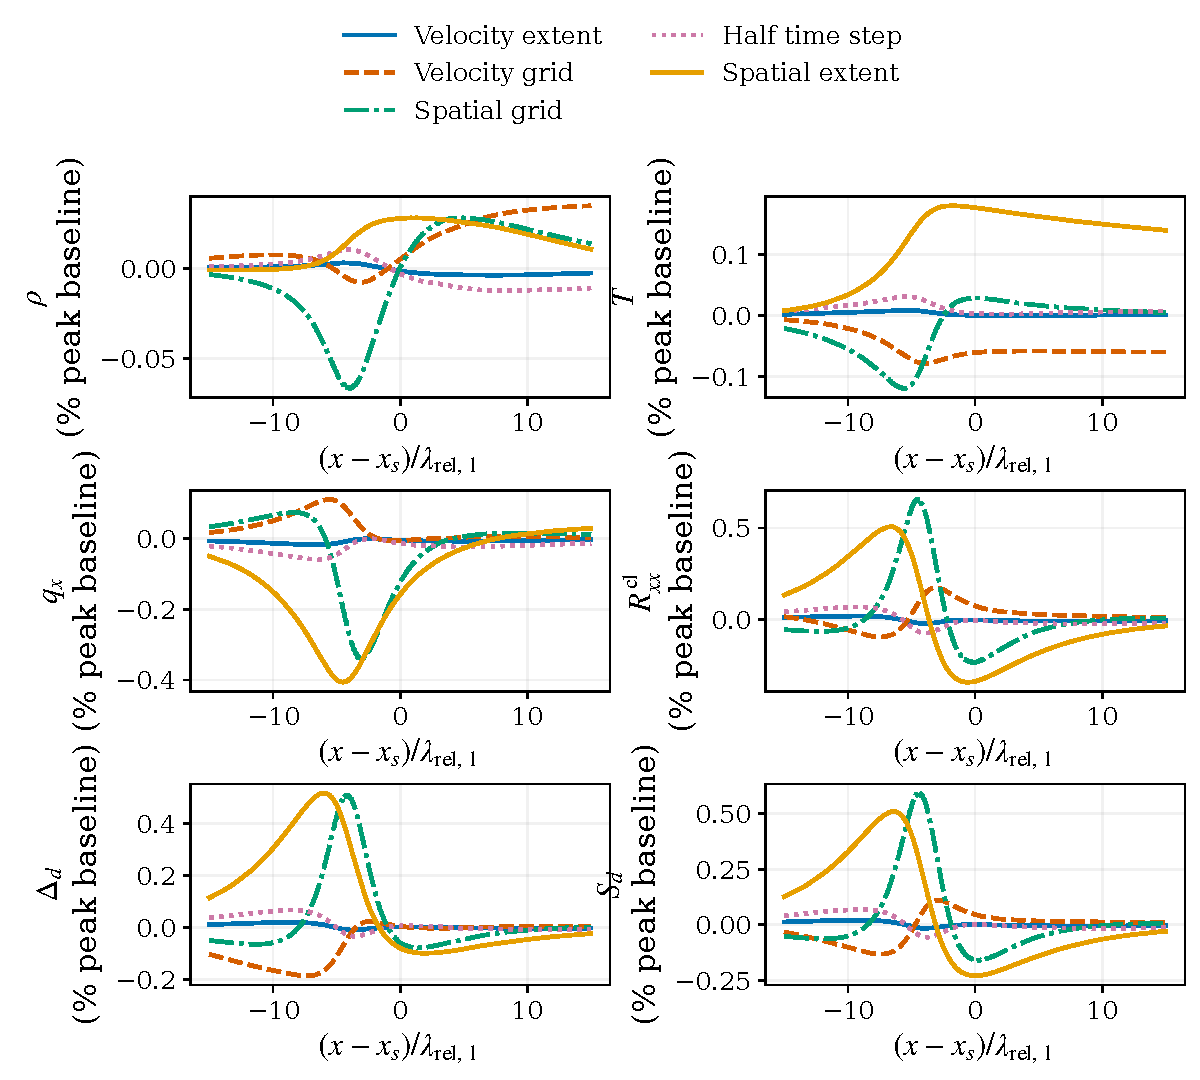
\includegraphics[width=\linewidth]{figures/A2_DVM_profile_differences.pdf}
\caption{Aligned DVM profile differences for the same tests as figure~\ref{fig:revision_dvm_summary}. Each ordinate is $100(g_{\rm test}-g_{\rm base})/\max|g_{\rm base}|$, with the maximum taken over the plotted interval. Peak normalisation avoids division by zero-crossing values. $\Delta_d$ uses the discrete-Maxwellian reference and is not the raw DSMC fourth-moment excess. This comparison does not directly measure omitted velocity-tail integrals or resolve distribution bimodality.}
\label{fig:revision_dvm_profiles}
\end{minipage}}
\endgroup
\end{figure}

\clearpage
\section{\revisionheading{DSMC particle-number sensitivity}}
\label{app:particle_sensitivity}

\begin{revision}
The seven PPC levels retain 400 spatial cells, time step 0.005 and 180000 steps, with sampling after step 70000 every tenth step. All eight seeds at each level use the original sampler. Figure~\ref{fig:revision_dsmc_source} holds this sampling schedule fixed and therefore does not establish averaging-window independence or reconfirm the historical collision-source/spatial-budget correlation of 0.987. Adjacent-PPC source differences are $10.870\%$, $3.589\%$, $4.963\%$, $2.275\%$, $1.268\%$ and $0.668\%$ for the successive pairs from 60--120 through 1920--3840. The trend need not be monotone because finite-seed noise and systematic effects remain. Collision counts are accumulated event counts, not independent sample counts or effective sample sizes.
\end{revision}

\begin{figure}
\centering
\begingroup\setlength{\fboxsep}{6pt}
\revisionbox{\begin{minipage}{0.92\textwidth}\captionsetup{width=\linewidth}
\centering
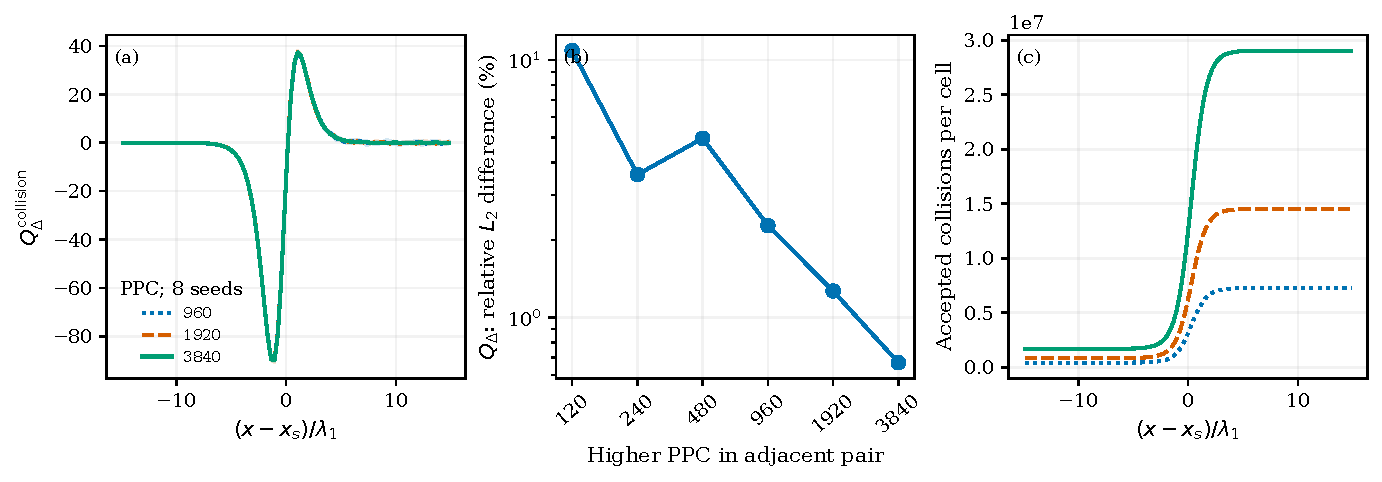
\includegraphics[width=\linewidth]{figures/A3_DSMC_collision_source.pdf}
\caption{Directly logged scalar collision-source sensitivity. (a) Eight-seed mean and pointwise $95\%$ Student-$t$ intervals for the three highest PPC levels. (b) Adjacent-PPC relative $L_2$ differences of aligned mean source profiles, normalised by the higher-PPC profile over $|(x-x_s)/\lambda_1|\leq15$. (c) Mean accumulated accepted-collision counts per cell, interpolated to the same aligned coordinate. No spatial smoothing is applied. Systematic pair-selection error is not included in the uncertainty bands.}
\label{fig:revision_dsmc_source}
\end{minipage}}
\endgroup
\end{figure}


\clearpage
\section{\revisionheading{Additional statistical and operator diagnostics}}
\label{app:additional_audits}
\begin{revision}
\textbf{Corrected pair selection.} A separate ensemble uses the corrected pair-selection implementation at PPC 120 and 960, with eight seeds per level and otherwise the same 400-cell grid, time step 0.005, 180000 steps and sampling schedule. Original and corrected checkpoints are version-specific. The original controls are reused; the corrected results are not substituted into the original PPC sequence. Each seed is aligned at the density midpoint before linear interpolation over $|(x-x_s)/\lambda_1|\leq15$. A bar denotes the mean over eight seed profiles. Suffixes $c$ and
$o$ identify corrected and original samplers; $s(g_c-g_o)$ is the
pointwise sample standard deviation of their eight matched-label
differences. For an observable $g$, the reported difference is $100\|\bar g_c-\bar g_o\|_2/\|\bar g_o\|_2$. A descriptive uncertainty scale is $100\|s(g_c-g_o)/\sqrt{8}\|_2/\|\bar g_o\|_2$, using matched seed labels. Random-number trajectories diverge after the algorithm change, so matching labels does not guarantee variance reduction.
The differences and their descriptive uncertainty scales are reported in table~\ref{tab:corrected_sampler}.
\par\medskip
\begin{minipage}{\linewidth}\captionsetup{width=\linewidth}
\makeatletter\def\@captype{table}\makeatother
\caption{Eight-seed corrected-versus-original DSMC sampler comparison. Entries are percentages. Differences use the original ensemble mean as the denominator; the descriptive uncertainty scale is the norm of the paired-label standard error, as defined in appendix~\ref{app:additional_audits}. Matching seed labels does not guarantee variance reduction. These values are not significance or equivalence tests.}
\label{tab:corrected_sampler}
\centering
\begin{tabular}{llrrrr}
\hline
PPC & Measure & $R^{\mathrm{cl}}_{xx}$ & $\Delta$ & $S$ & $Q_\Delta$\\
\hline
120 & Difference & 3.611 & 2.851 & 3.288 & 3.524\\
    & Uncertainty scale & 3.304 & 2.497 & 2.869 & 3.859\\
960 & Difference & 0.933 & 0.734 & 0.800 & 1.413\\
    & Uncertainty scale & 0.971 & 0.718 & 0.809 & 1.296\\
\hline
\end{tabular}
\end{minipage}
\par\medskip

Thus the sub-percent moment differences at PPC 960 are comparable to sampling uncertainty. This is not an equivalence test, a proof that the correction has no effect, or a convergence study of the corrected sampler.

\textbf{Sampling-window diagnostic.} For the eight original PPC-3840 seeds, ten disjoint 10000-step blocks are reconstructed over steps 80000--180000. Moment sums are differenced using sample counts; collision-source sums use their accumulated sampling-time exposure. Each block is independently aligned. Differences between the ensemble means of the first and last five blocks are $0.285\%$, $0.262\%$, $0.193\%$ and $1.034\%$ for $R^{\cl}_{xx},\Delta,S,Q_\Delta$, respectively. Ten blocks do not establish full independence or a reliable effective sample size. Percentile intervals of a nonnegative norm cannot be interpreted as tests of zero drift.

\textbf{Velocity tails and entropy.} Twenty selected spatial rows of each Mach-5 baseline, enlarged-velocity-domain and refined-velocity-grid final distribution were inspected. These sampled tail diagnostics do not cover the Mach-6, Mach-8 or Mach-12 distributions. The largest resolved $|\boldsymbol c|^4 f$ fraction in the outer ten percent of the velocity box was approximately $3\times10^{-8}$ for the baseline/refined grids and $4.4\times10^{-12}$ for the enlarged box. These are resolved outer-box contributions, not certified bounds on omitted tails beyond the computational domain.

The local ES-FP operator was evaluated on these BGK reference distributions using the full temperature tensor, $\beta=-5/4$ and unit collision rate. On the twenty inspected rows of each Mach-5 case, the minimum eigenvalue of $D/(2\nu T)$ was approximately $0.11160$ for the baseline, $0.11157$ for the enlarged velocity domain and $0.11239$ for the refined velocity grid. Diffusion was therefore positive definite at these sampled states. This selected-row check does not establish admissibility at every spatial point, for the legacy Mach-2/3 profiles, or during an ES-FP evolution. Second- and fourth-order derivatives of $\log f$, boundary entropy fluxes, integration-by-parts defects and same-grid continuum-Maxwellian controls were compared. Computed shock-core entropy production was positive, but derivative-order sensitivity was $15.93\%$ on the baseline grid and $9.17\%$ on the refined grid. The maximum core energy-source residual, normalised by $\rho T$, decreased from 0.103 to 0.01995 in these rate units. Negative upstream values on the coarse grid also occurred for its Maxwellian control; they cannot be identified as physical entropy violations. Conversely, these diagnostics do not establish an H-theorem or an entropy-stable ES-FP shock solution.

\textbf{Shakhov clipping budget.} In the separate 20-sweep diagnostic, maximum single-event clipping increments normalised by $\rho$, $\rho T$ and $\rho T^2$ were $4.695\times10^{-5}$ for mass, $1.327\times10^{-3}$ for energy and $7.889\times10^{-3}$ for the fourth scalar moment. These maxima are not accumulated errors at a fixed cell or steady-state error estimates. Clipping is therefore not assumed to preserve the analytic source-neutrality property of the unmodified Shakhov correction.
\end{revision}


\clearpage
\section{\revisionheading{High-particle DSMC profiles and cross-method context}}
\label{app:dsmc_cross_method}
\begin{revision}
The Shakhov DVM curves in this appendix are a separate $Pr=2/3$ campaign, not the $Pr=1$ BGK budget references. The reduced distributions are $g=\int f\,\dd v_y\dd v_z$, $h=\int(v_y^2+v_z^2)f\,\dd v_y\dd v_z$ and $k=\int(v_y^2+v_z^2)^2f\,\dd v_y\dd v_z$; retaining $k$ permits the axial fourth-order quantities to be evaluated. Uniform cell-centred spatial grids and longitudinal composite-trapezoidal quadrature are used. Streaming is first-order explicit upwind with $\Delta t=0.8\Delta x/v_{\max}$. The local collision update uses the exponential relaxation factors $\exp(-\Delta t/\tau)$ and $\exp(-Pr\Delta t/\tau)$, with $\mu=T$, $\tau=1/\rho$, and no distribution clipping. Incoming populations are supplied by the upstream and downstream Rankine--Hugoniot Maxwellian reservoirs; outgoing populations come from the interior. The plotted Mach-2 profile has 1280 cells on $[-30,30]$ and 321 longitudinal velocities on $[-16,16]$. The Mach-3, Mach-4 and Mach-5 profiles use 1920, 2560 and 3200 cells on $[-45,45]$, $[-60,60]$ and $[-75,75]$, respectively, with 801 velocities on $[-40,40]$. Their saved times are $238.125$, $173.4375$ and $143.4375$. These are the archived plotted snapshots, not a claim that subsequently evolving jobs remained at those times.

For this campaign, stationarity requires five consecutive checks with the maximum fieldwise relative change below $10^{-7}$ over all eight saved fields $(\rho,u_x,T,q_x,\sigma_{xx},R^{\cl}_{xx},\Delta,S)$, with each denominator bounded below by $10^{-8}$. Checks are separated by approximately two computational time units. The plotted Mach-3--5 receipts have zero qualifying consecutive checks. This criterion differs from that of the separate Mach-8 benchmark in appendix~\ref{app:m8_reference}.

The corrected-Shakhov R26 comparison uses the same $Pr=2/3$ and $\mu=T$, $\tau=1/\rho$ transport parameters, but solves a steady moment boundary-value problem. For the archived Mach-3 result, a piecewise degree-four representation on 4012 elements gives 16049 native points over $[-45,45]$, with an eight-point Gauss residual objective and a sparse augmented Levenberg--Marquardt solve. Independent qualification evaluates the full corrected tensor PDE on the native points, finite profiles and positive pressure, with scaled PDE and boundary/phase tolerances $0.01$ and $10^{-4}$. The measured native PDE residual is $0.0046433$ and the boundary/phase residual $1.51\times10^{-11}$. The runner stopped at its 30-iteration limit with automatic acceptance disabled; the separate independent checker subsequently passed the stated numerical criteria. Thus ``accepted'' here denotes this finite-tolerance independent qualification, not a zero residual, uniqueness, or agreement with a kinetic collision operator. The Mach-2 corrected profile has 3841 native points. Only these two corrected R26 profiles enter the present cross-method comparison; no corrected Mach-4 or Mach-5 R26 solution is included.
\end{revision}
\begin{revision}
We add a separate Bird DSMC profile set at $M_1=2,3,4,5$, with 2000 upstream particles per cell, 800 spatial cells, $\Delta t=0.005$, and sampling through $t=400$ after a warm-up to $t=200$ \citep{Bird1994}. The collision model is VHS with $\omega=1$ and inverse scattering parameter $\alpha_{\rm VSS}=1$ in the variable soft sphere (VSS) notation (isotropic scattering);
 $\omega$ is the viscosity exponent and
starred quantities are divided by their corresponding upstream references; the transport law is $\mu^*=T^*$ and $\tau^*=1/\rho^*$. Each Mach number has one independent seed, 800 total blocks, and 400 sampled blocks after warm-up. The high-particle runs use the original Bird sampler, so the pair-selection limitation described in appendix~\ref{app:additional_audits} remains applicable.

For the Mach-2 quantitative comparison, profiles are aligned by a density-midpoint translation only and evaluated on the common interval $[-15,15]\lambda_1$, without fitting the shock width. Table~\ref{tab:dsmc2000_m2} reports raw-profile relative $L^2$ differences with the DSMC norm in the denominator. The comparison is descriptive: the DSMC samples are finite-time, one-seed estimates, stationarity is not certified, and higher central moments retain finite-sample bias. The DVM is a Shakhov calculation and the R26 curve is the corrected consistent Shakhov solution; equal transport coefficients do not make these collision descriptions identical.

Figures~\ref{fig:dsmc2000_m2} and~\ref{fig:dsmc2000_m3m5} show the profiles. The Mach-2 figure uses raw DSMC data; the Mach-3--5 figure also shows local quadratic smoothing as a visual guide. All tabulated errors use unsmoothed profiles. The DVM curves are finite-time snapshots, not stationary references. Corrected-Shakhov R26 profiles are available and numerically accepted here at Mach 2 and 3 only; no corrected R26 result is supplied at Mach 4 or 5. Here $e_R=R^{\cl}_{xx,\rm model}-R^{\cl}_{xx,\rm DSMC}$,
$e_{\Delta/3}=(\Delta_{\rm model}-\Delta_{\rm DSMC})/3$ and
$e_S=S_{\rm model}-S_{\rm DSMC}$; $\langle a,b\rangle=\sum_i a_ib_i$
on the comparison interval, and $c_e$ denotes their normalised inner
product. Table~\ref{tab:dsmc2000_channel} resolves the signed errors in $S=R^{\cl}_{xx}+\Delta/3$. The Mach-3 R26 row was recomputed from the accepted corrected-Shakhov profile, rather than read from a figure annotation. With the same raw-data alignment, its relative $L^2$ differences against 2000-ppc DSMC are $1.328\%$, $2.613\%$, $15.267\%$, $38.376\%$, $26.390\%$ and $26.449\%$ for $\rho,T,q_x,R^{\cl}_{xx},\Delta,S$, respectively. These comparisons provide a reusable cross-method profile benchmark, not a validation of the collision-production measurement, a statistical confidence interval, or a test of the two-channel identifiability result.
\end{revision}

\begin{table}
\centering
\revisionbox{\begin{minipage}{0.90\linewidth}\captionsetup{width=\linewidth}\caption{Mach-2 raw-profile relative $L^2$ differences against the 2000-particle-per-cell Bird DSMC result. Entries are $100\|g_{\rm model}-g_{\rm DSMC}\|_2/\|g_{\rm DSMC}\|_2$ on the common $[-15,15]\lambda_1$ interval after density-midpoint translation only; no shock-width fit or smoothing is used in the metric. The DVM is a finite-time Shakhov snapshot and the R26 result is the corrected Shakhov profile.}
\label{tab:dsmc2000_m2}\end{minipage}}\par
\small
\begin{tabular}{lrrrrrr}
\toprule
Model & $\rho$ & $T$ & $q_x$ & $R^{\cl}_{xx}$ & $\Delta$ & $S$\\
\midrule
Shakhov DVM & 0.141 & 0.180 & 2.968 & 16.718 & 25.948 & 8.272\\
Corrected Shakhov R26 & 0.468 & 0.561 & 6.165 & 22.883 & 25.755 & 11.963\\
\bottomrule
\end{tabular}
\end{table}

\begin{table}
\centering
\revisionbox{\begin{minipage}{0.90\linewidth}\captionsetup{width=\linewidth}\caption{Signed-error decomposition against raw 2000-ppc DSMC profiles at Mach 2 and 3. The three error columns are $100\|e\|_2/\|S_{\rm DSMC}\|_2$ on $[-15,15]\lambda_1$ after density-midpoint translation only; $c_e=\langle e_R,e_{\Delta/3}\rangle/(\|e_R\|_2\|e_{\Delta/3}\|_2)$. Thus $e_S=e_R+e_{\Delta/3}$ pointwise. The Mach-3 DVM row uses the saved transient snapshot at $t=238.125$. The R26 Mach-3 row comes from the accepted corrected-Shakhov profile (SHA-256 beginning \texttt{1b870043}); the calculations use unsmoothed profiles and are descriptive finite-time comparisons.}
\label{tab:dsmc2000_channel}\end{minipage}}\par
\small
\begin{tabular}{llrrrr}
\toprule
$M_1$ & Model & $\|e_R\|$ (\%) & $\|e_{\Delta/3}\|$ (\%) & $\|e_S\|$ (\%) & $c_e$\\
\midrule
2 & Shakhov DVM & 8.424 & 13.906 & 8.272 & $-0.836$\\
2 & Corrected Shakhov R26 & 11.531 & 13.803 & 11.963 & $-0.567$\\
3 & Shakhov DVM & 8.837 & 13.589 & 9.189 & $-0.742$\\
3 & Corrected Shakhov R26 & 19.440 & 14.181 & 26.449 & $+0.219$\\
\bottomrule
\end{tabular}
\end{table}

\begin{figure}
\centering
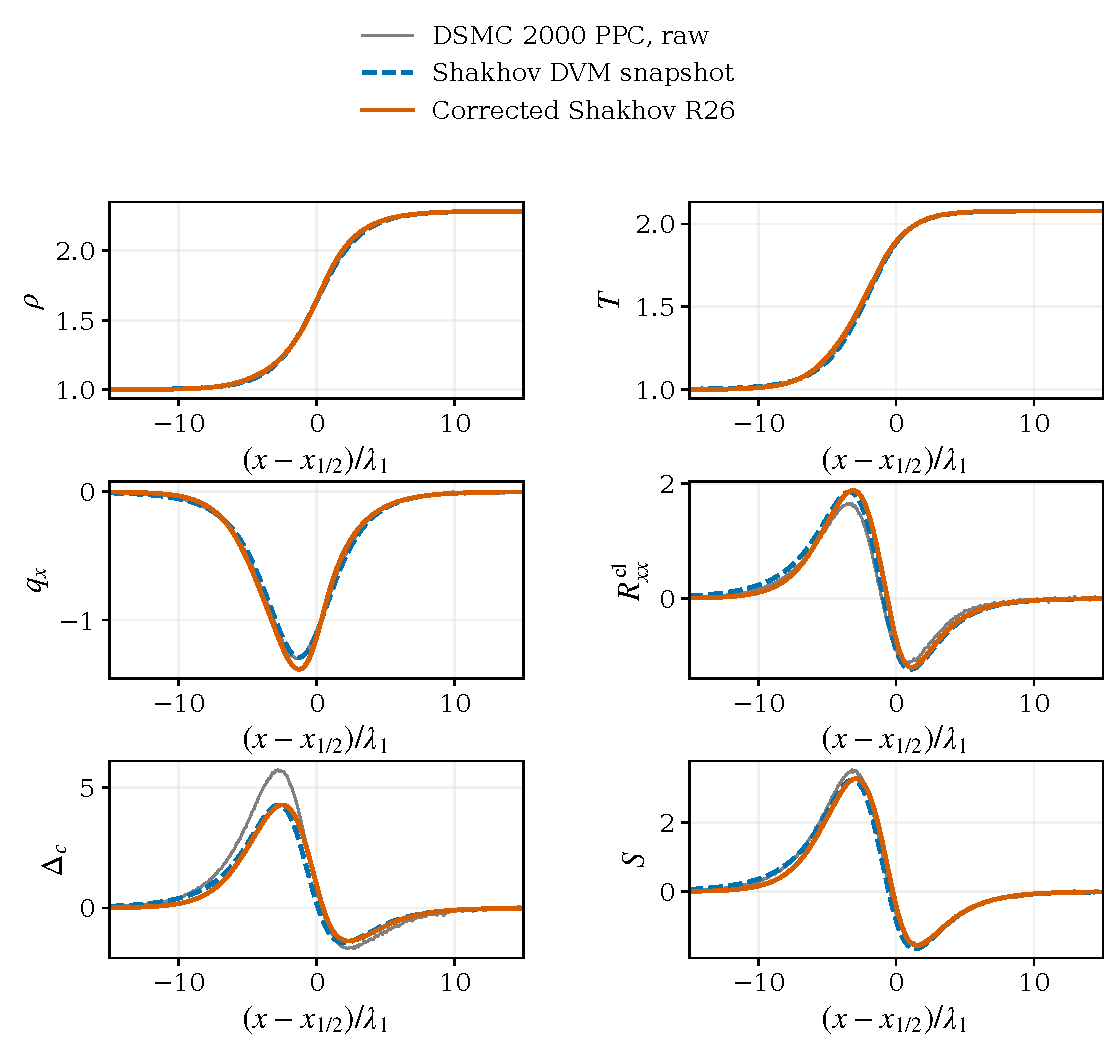
\includegraphics[width=\linewidth]{figures/M2_DSMC2000_cross_method.pdf}
\caption{Mach-2 raw profiles from 2000-ppc Bird DSMC, a Shakhov DVM snapshot, and corrected-Shakhov R26. Density-midpoint translation is the only spatial alignment; the historical R26 curve preceding the symmetric trace-free (STF) corrections is excluded.}
\label{fig:dsmc2000_m2}
\end{figure}

\begin{figure}
\centering
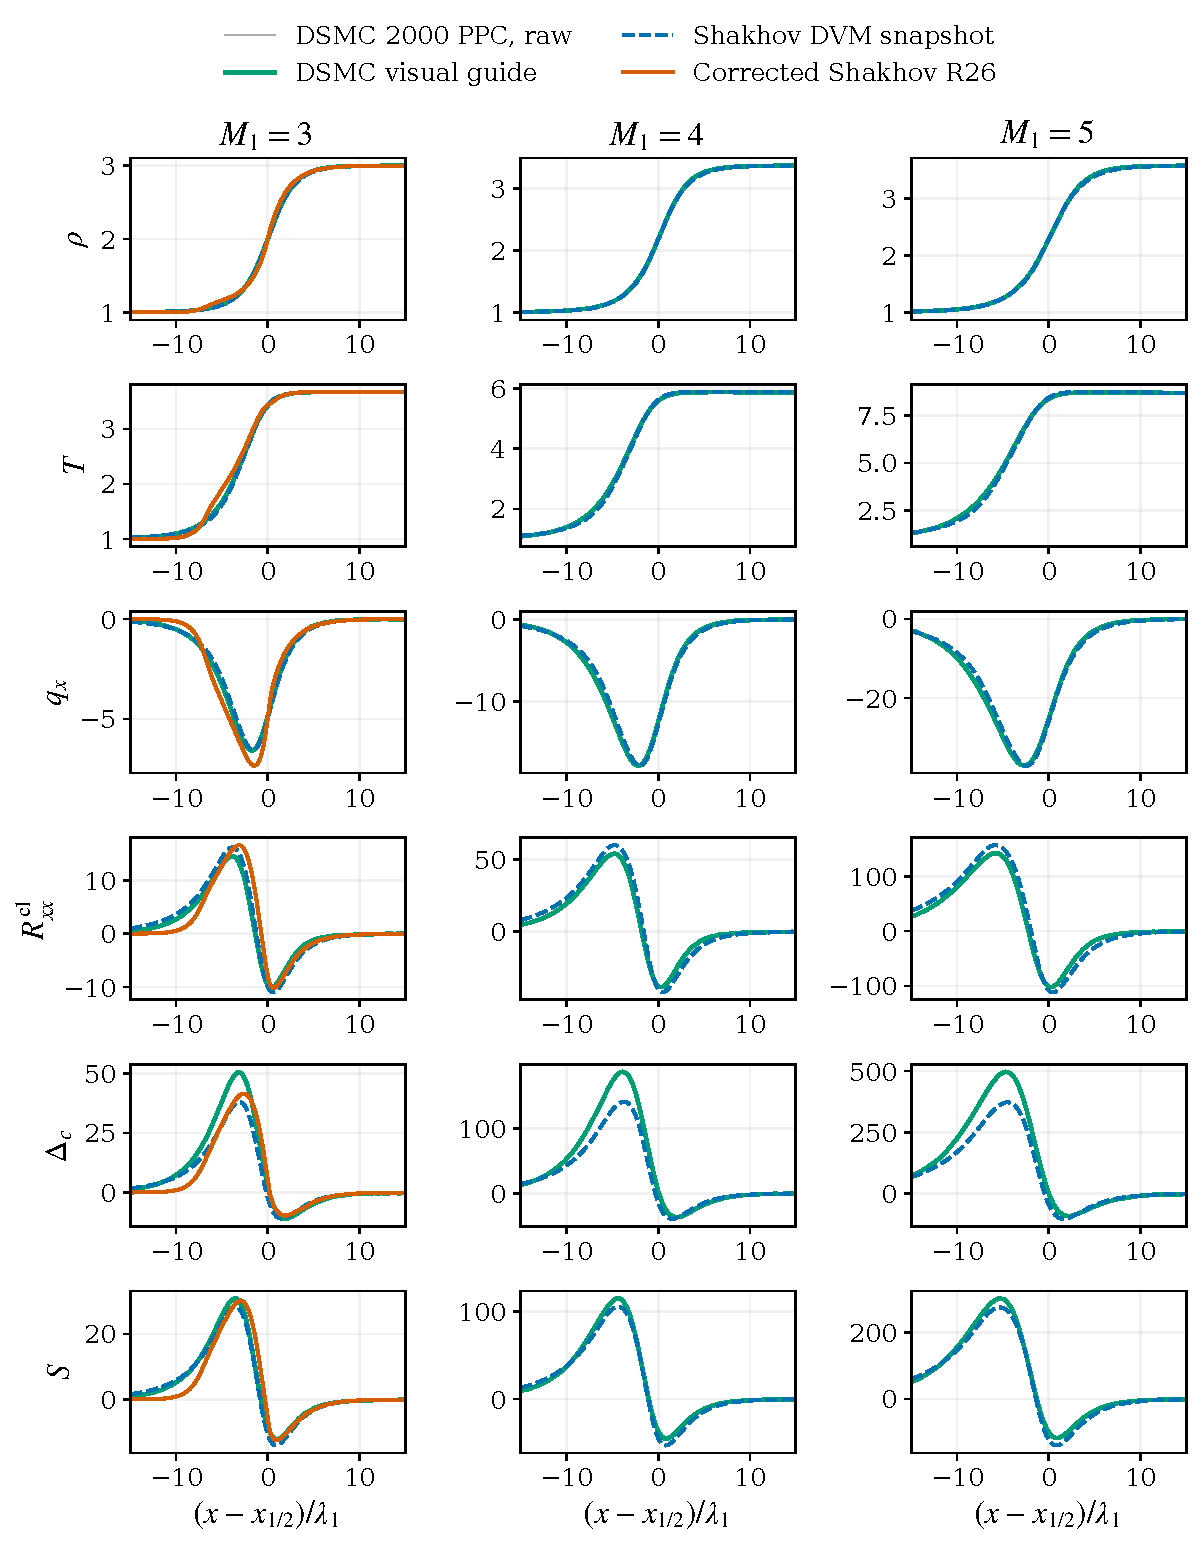
\includegraphics[width=\linewidth]{figures/M3_M5_DSMC2000_DVM_R26.pdf}
\caption{Mach-3--5 profile comparison using 2000-ppc Bird DSMC and Shakhov DVM snapshots, with the corrected-Shakhov R26 profile shown only where available (Mach 3). Raw DSMC data and display-only local smoothing are both shown. The DVM fields are transient snapshots; neither the DSMC stationarity nor model-specific convergence is certified.}
\label{fig:dsmc2000_m3m5}
\end{figure}

\clearpage

\clearpage
\section{\revisionheading{Mach-8 Shakhov benchmark comparison}}
\label{app:m8_reference}
\begin{revision}
This appendix compares density and temperature with the S-model curves in figure~1 of \citet{ChenXuCai2013}. The matched physical parameters are $M_1=8$, $Pr=2/3$, $\omega=0.81$ in $\mu\propto T^\omega$, and $\rho_1=T_1=R=\lambda_1=1$. Equation~(35) of that reference gives $\mu_{\rm ref}=1.0338373584$ and hence $\tau=\mu_{\rm ref}T^{\omega-1}/\rho$. Our calculation solves transverse-integrated Shakhov equations for $g=\int f\,\dd v_y\dd v_z$ and $h=\int(v_y^2+v_z^2)f\,\dd v_y\dd v_z$, without clipping. The baseline uses 1200 spatial cells on $[-50,30]\lambda_1$ and 401 longitudinal velocities on $[-40,40]$, in double precision. Its first-order upwind discretisation differs from the reference unified gas-kinetic scheme (UGKS) discretisation with 300 spatial cells. This is a separate Mach-8 calculation from the three-dimensional-velocity BGK configurations in table~\ref{tab:high_mach_grids}: its collision model, relaxation law and reduced velocity representation differ, so the spatial and velocity extents are not interchangeable.

The published curves are extracted from the original PDF vector paths (133 vertices per curve), rather than supplied numerical data. Density and temperature are normalised by their Rankine--Hugoniot jumps. One translation aligns each computed density midpoint with the reference density midpoint; the same translation is used for temperature, with no fitted stretching or independent temperature shift. At the reference vertices over $-20\leq x/\lambda_1\leq15$, the maximum absolute discrepancy, expressed as a percentage of the full jump, is reported in table~\ref{tab:m8_reference}. Figure~\ref{fig:m8_reference} shows both profiles and differences. Finite resolution of the published curves and interpolation introduce unquantified extraction uncertainty, so sub-percent differences should not be interpreted as exact solver errors.
\end{revision}
\begin{revision}
\par\medskip
\noindent\begin{minipage}{\linewidth}\captionsetup{width=\linewidth}
\makeatletter\def\@captype{table}\makeatother
\captionsetup{width=\linewidth,justification=raggedright,singlelinecheck=false}
\caption{Mach-8 comparison with the published Shakhov curves. Maximum discrepancies are percentages of the full density or temperature jump, after a shared density-midpoint alignment. The refined case doubles the spatial resolution and also halves the CFL time step.}
\label{tab:m8_reference}
\centering
\begin{tabular}{lrr}
\hline
Calculation & Density & Temperature\\
\hline
Baseline, $t=400$ & 0.97 & 1.09\\
Extended time, $t=800$ & 0.97 & 1.09\\
Spatial refinement, $N_x=2400$, $t=400$ & 0.78 & 0.99\\
\hline
\end{tabular}
\end{minipage}
\end{revision}
\begin{figure}
\centering
\begingroup\setlength{\fboxsep}{6pt}
\revisionbox{\begin{minipage}{0.92\textwidth}\captionsetup{width=\linewidth}
\centering
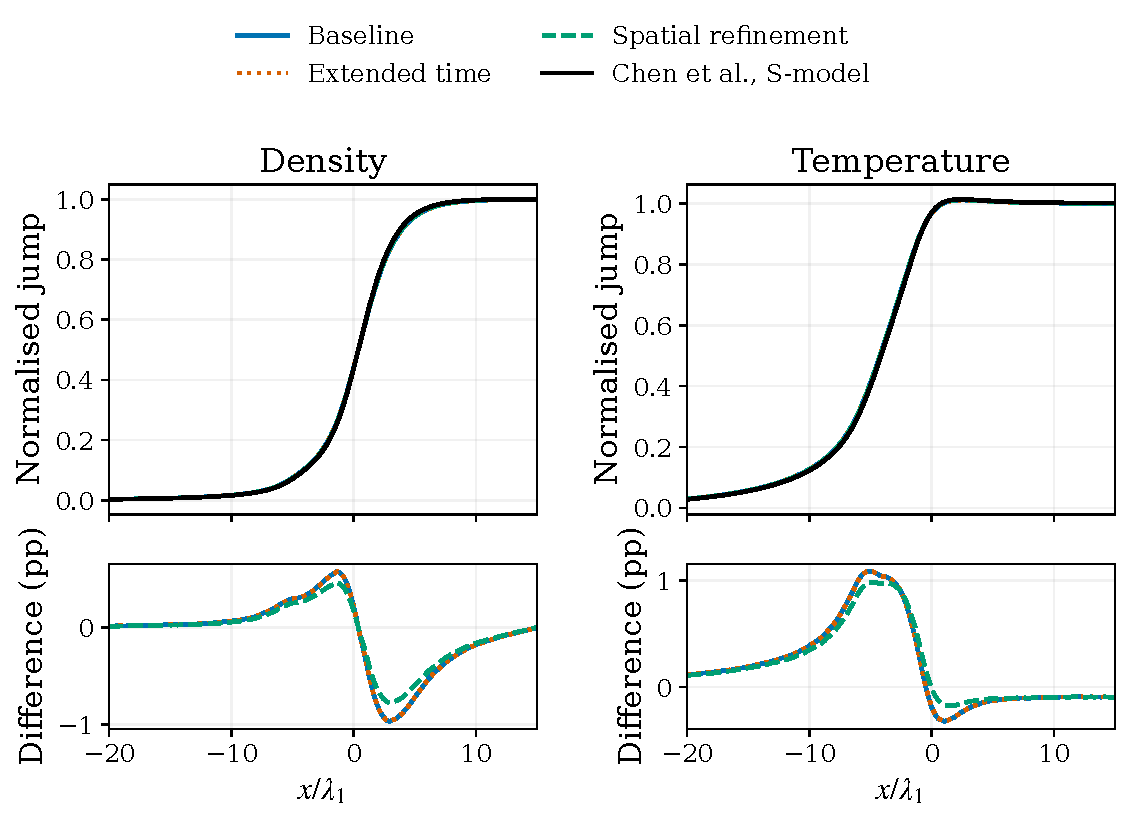
\includegraphics[width=\linewidth]{figures/m8_paper_comparison.pdf}
\caption{Matched-parameter Mach-8 Shakhov benchmark comparison. Black curves are the vector-extracted S-model results from figure~1 of \citet{ChenXuCai2013}; coloured curves are the present baseline, time-extended and spatially refined calculations. Lower panels show discrepancies in percentage points of the normalised jump. Density and temperature use the same spatial translation for each calculation.}
\label{fig:m8_reference}
\end{minipage}}\endgroup
\end{figure}
\begin{revision}
The close macroscopic agreement is a bounded benchmark check, not validation of a nonnegative kinetic distribution or of the fourth-order channels. Here $Y$ denotes any field in the five-field list below. In all cases the prescribed stationarity criterion remains unmet: every 2000 steps, the maximum profile change over $(\rho,u_x,T,q_x,\sigma_{xx})$, divided fieldwise by $\max(1,\max_x|Y|)$, must be below $10^{-7}$ for five consecutive checks on the fixed spatial grid. The integrations terminate at their prescribed physical times. A small translation of the shock contributes to this unaligned criterion even when aligned profiles are close.

The six sensitivity calculations test extended integration time, finer spatial resolution, a smaller time step, finer velocity resolution, a larger velocity domain and a larger spatial domain. The table and figure report comparisons for the baseline, extended-time and spatially refined calculations. Across the six tests, the maximum local negative-$g$ mass fraction remains approximately $2.13$--$2.15\%$, and the corresponding negative-$h$ energy fraction is $5.15$--$5.22\%$. Small aligned macroscopic sensitivities do not remove this positivity limitation. The reduced distributions also do not determine all three-dimensional fourth-order moments. This appendix therefore supports the reported density/temperature comparison only; it does not independently validate $R^{\cl}_{xx}$, $\Delta$ or $S$, or replace the constant-relaxation BGK high-Mach results in \S\ref{sec:high_mach}.
\end{revision}


\clearpage
\section{\revisionheading{Normal-shock symmetry and supporting moment identities}}
\label{app:symmetry_proof}

\begin{revision}
\textbf{Symmetry assumptions.} The planar normal-shock problem has no transverse flow, forcing or preferred transverse direction. Its Maxwellian reservoirs and isotropic collision law are invariant under transverse reflections and rotations. We consider the solution branch that preserves these symmetries, as does evolution from symmetry-preserving initial data. This specifies the branch; it is not a uniqueness theorem for every steady solution of the kinetic boundary-value problem. At each fixed $x$, write $c_y=v_y$, $c_z=v_z$ and $c_x=v_x-u_x(x)$. The following three symmetries suffice for the moment reduction:
\begin{equation}
\begin{split}
 f(c_x,c_y,c_z)&=f(c_x,-c_y,c_z)=f(c_x,c_y,-c_z),\\
 f(c_x,c_y,c_z)&=f(c_x,c_z,c_y).
\end{split}
\label{eq:transverse_symmetries}
\end{equation}
The local equilibrium reference has the same symmetries. No reflection symmetry in $c_x$ is assumed: the streamwise heat flux may therefore be non-zero.
\end{revision}

\begin{revision}
\textbf{Componentwise proof.} Extend \eqref{eq:q_sigma} and \eqref{eq:Rdef} to the full tensors, with $\delta_{ij}$ the Kronecker delta:
\begin{equation}
\begin{split}
 C_{ij}(\boldsymbol c)&=c_i c_j-\tfrac13|\boldsymbol c|^2\delta_{ij},
 \qquad \sigma_{ij}=\int C_{ij}f\,\dd\boldsymbol v,\\
 R^{\cl}_{ij}&=\int |\boldsymbol c|^2 C_{ij}(f-M_d)\,\dd\boldsymbol v
                 -7T\sigma_{ij}.
\end{split}
\label{eq:full_R_tensor}
\end{equation}
For $i\ne j$, $C_{ij}=c_i c_j$. Changing $c_y\to-c_y$ reverses the sign of the $xy$ and $yz$ integrands without changing $f$, $M_d$ or the integration measure; changing $c_z\to-c_z$ does the same for $xz$. Each such integral equals its negative and is zero. This proves that the off-diagonal components of both $\sigma$ and $R^{\cl}$ vanish. Next, changing variables $c_y\leftrightarrow c_z$ interchanges the $yy$ and $zz$ integrands while leaving the distributions and measure unchanged, giving equality of their integrals. Finally, the pointwise identity
\[
 \sum_{i=x,y,z} C_{ii}=|\boldsymbol c|^2-|\boldsymbol c|^2=0
\]
implies $\sum_i\sigma_{ii}=0$ and $\sum_i R^{\cl}_{ii}=0$, including the stress subtraction. Combining these facts yields
\begin{equation}
 R^{\cl}_{yy}=R^{\cl}_{zz}=-\tfrac12R^{\cl}_{xx},\qquad
 \sigma_{yy}=\sigma_{zz}=-\tfrac12\sigma_{xx},\qquad
 R^{\cl}_{ij}=\sigma_{ij}=0\quad(i\ne j).
 \label{eq:normal_shock_tensor_reduction}
\end{equation}
Consequently $\tr(\sigma^2)=\sigma_{xx}^2+2(\sigma_{xx}/2)^2=3\sigma_{xx}^2/2$, as used in \eqref{eq:es_1d_delta_target}. These restrictions leave $\Delta$ independent: it is a scalar integral, not the trace of the already trace-free tensor $R^{\cl}$. For example, on full velocity space with continuum-reference moments, a mixture of isotropic Maxwellians with different temperatures and the same mean velocity has $R^{\cl}_{ij}=\sigma_{ij}=0$. For positive mixture fractions $a_\ell$ summing to one and component temperatures $T_\ell$, the mixture temperature is $T=\sum_\ell a_\ell T_\ell$ and $\Delta_c=15\rho[\sum_\ell a_\ell T_\ell^2-T^2]>0$ when the temperatures differ. This illustrates independence at the level of moment definitions, not an additional shock solution.
\end{revision}

\begin{revision}
\textbf{Discrete velocities.} The same change-of-variables proof becomes a node-pairing proof when the transverse node sets and weights are invariant under sign changes and interchange, and the sampled distribution and fitted $M_d$ preserve those symmetries. Equal $y$ and $z$ grids symmetric about zero admit these pairings; invariance under arbitrary rotations is unnecessary. The trace identity holds nodewise even on a finite grid. The other equalities require the stated symmetries and are subject to numerical symmetry errors; finite-particle DSMC samples need not satisfy them exactly. In particular, symmetry enforces equality of the two transverse stresses, not vanishing diagonal stress of a finite-grid Maxwellian. It does not remove the equilibrium-quadrature defects reported in table~\ref{tab:high_mach_run_audit}.
\end{revision}

\newpage
\begin{revision}
\textbf{Why the coefficient $7$?} It is a continuum R26 moment convention. Let $M$ be the Maxwellian with covariance $T I$ and consider only its standard stress-polynomial contribution
\[
 f_\sigma=M\frac{\sigma_{kl}c_kc_l}{2\rho T^2},\qquad \sigma_{kk}=0,
\]
where repeated indices are summed. Gaussian contraction gives
\begin{equation}
 \int |\boldsymbol c|^2c_ic_jc_kc_l M\,\dd\boldsymbol v
 =7\rho T^3(\delta_{ij}\delta_{kl}+\delta_{ik}\delta_{jl}
                         +\delta_{il}\delta_{jk}).
 \label{eq:gaussian_sixth_contraction}
\end{equation}
To verify the factor, write $|\boldsymbol c|^2=\sum_a c_a^2$: in the Gaussian pairings of $c_a c_a c_i c_j c_k c_l$, pairing the two $a$ indices together contributes the dimension $3$, while the remaining pairings contribute $4$, giving $3+4=7$ for each displayed Kronecker product. Contracting with $\sigma_{kl}/(2\rho T^2)$ removes the first product and gives $7T\sigma_{ij}$. The scalar trace contribution vanishes under the same contraction, so
\[
 \int |\boldsymbol c|^2 C_{ij}f_\sigma\,\dd\boldsymbol v=7T\sigma_{ij}.
\]
Subtracting this contribution defines the fourth-order departure used in \eqref{eq:full_R_tensor}; it does not assume the actual shock distribution equals a truncated Grad expansion. On a finite grid the Gaussian contraction need not be exact. The discrete-reference definition retains the coefficient $7$ as the chosen moment convention, with the separate $M_d$ subtraction explicitly specified in \eqref{eq:Rdef}.
\end{revision}

\clearpage

\clearpage
\section{\revisionheading{Independently evolved ES-BGK shocks at Mach 2 and 3}}
\label{app:esbgk_evolved}
\begin{revision}
The source evaluations in \S\ref{sec:delta_budget} are supplemented by independent ES-BGK shock evolutions. These calculations use the anisotropic Gaussian target in \eqref{eq:es_gaussian}, rather than substituting its source into a saved BGK solution. The upstream state is $\rho_1=T_1=1$, $R=1$, $\gamma=5/3$ and $u_1=M_1\sqrt{5/3}$; incoming populations at the two boundaries are equilibrium Rankine--Hugoniot reservoirs. With $Pr=2/3$ and $\alpha_{\rm ES}=1-1/Pr=-1/2$, viscosity matching to the Shakhov law $\mu=T$ requires
\begin{equation}
 \tau_{\rm ES}=(1-\alpha_{\rm ES})\frac{\mu}{p}
 =\frac{3}{2\rho},\qquad p=\rho T.
\end{equation}
Using $\tau_{\rm ES}=\mu/p$ would give a different viscosity. Positions use the shared Shakhov upstream relaxation-length reference, $\lambda_1=\sqrt{RT_1}\tau_{\rm Sh,1}=1$ in computational units; the different ES-BGK relaxation time is not used to rescale the plotted coordinates.

The implemented kinetic solver evolves three reduced distributions,
$g=\int f\,\dd v_y\dd v_z$, $h=\int(c_y^2+c_z^2)f\,\dd v_y\dd v_z$ and $k=\int(c_y^2+c_z^2)^2f\,\dd v_y\dd v_z$.
Normal-shock symmetry gives zero transverse mean velocity. The transverse Gaussian target integrals are evaluated analytically: $h_G=2T_\perp g_G$ and $k_G=8T_\perp^2g_G$, with $T_\parallel=T+\alpha_{\rm ES}\sigma_{xx}/\rho$ and $T_\perp=T-\alpha_{\rm ES}\sigma_{xx}/(2\rho)$. This reduction retains the axial and contracted fourth moments used here. Spatial transport uses conservative first-order upwind finite volumes with one shared interface flux; collision uses a self-consistent backward-Euler update with implicit stress relaxation. The axial velocity interval is $[-40,40]$, with trapezoidal quadrature. There is no clipping, silent normalisation or periodic recentering in these ES-BGK calculations.

The Mach-2 and Mach-3 domains are $[-30,30]$ and $[-45,45]$, respectively. Baseline cells have $\Delta x=0.1875$, axial velocity spacing $\Delta v=0.2$ and $\Delta t=0.00375$ ($C_{\rm CFL}=0.8$). The spatial-refinement cases halve both $\Delta x$ and the CFL-selected time step; velocity refinement then halves $\Delta v$ at that finer spatial grid. Thus the baseline-to-spatial-refinement comparison changes space and time together. The six completed cases in table~\ref{tab:esbgk_evolved} terminate at $t\simeq400$. Separate half-time-step checks and subsequent continuations are excluded from this frozen result set because they were not completed at the time of this deposit.

Stationarity requires five consecutive comparisons approximately two physical-time units apart, with the largest scaled change in each of $\rho,u_x,T,q_x,\sigma_{xx},R^{\cl}_{xx},\Delta,S$ below $10^{-7}$ and the scaled moment rate from a full numerical step below $10^{-7}$. Each family is scaled by its maximum absolute value, with a $10^{-8}$ denominator floor. An additional numerical step at the final saved state measures the reported post-state RHS. None of these six cases passes this criterion: their final rates remain between $5.5\times10^{-5}$ and $6.2\times10^{-5}$. Positive density, temperature, target covariance and reduced populations are retained, but successful execution and positivity do not certify a stationary shock or global stability.
\end{revision}

\par\medskip\noindent\begin{minipage}{\linewidth}\makeatletter\def\@captype{table}\makeatother
\centering
\revisionbox{\begin{minipage}{0.96\textwidth}\captionsetup{width=\linewidth}
\caption{Completed finite-time ES-BGK cases at $Pr=2/3$, $t\simeq400$. B denotes baseline, X coupled spatial/time refinement, and V subsequent axial-velocity refinement. $N_x$ counts cells and $N_v$ axial velocity nodes. The three errors are percentages relative to direct velocity moments on the common mask $|S_{\rm direct}|>0.02\max|S_{\rm direct}|$. They measure steady-form budget reconstruction of a nonstationary snapshot, not ES-BGK model error. RHS is the final scaled full-step moment rate.}
\label{tab:esbgk_evolved}
\centering\small\setlength{\tabcolsep}{3pt}
\begin{tabular}{lrrr rrr r}
\toprule
Case & $N_x$ & $N_v$ & $\Delta t$ & $\varepsilon_S$ & $\varepsilon_\Delta$ & $\varepsilon_R$ & RHS\\
\midrule
M2 B & 320 & 401 & 0.003750 & 13.70 & 16.62 & 26.62 & $6.15\times10^{-5}$\\
M2 X & 640 & 401 & 0.001875 & 6.80 & 8.46 & 13.24 & $6.15\times10^{-5}$\\
M2 V & 640 & 801 & 0.001875 & 6.82 & 8.47 & 13.27 & $6.15\times10^{-5}$\\
M3 B & 480 & 401 & 0.003750 & 8.35 & 12.10 & 17.19 & $5.53\times10^{-5}$\\
M3 X & 960 & 401 & 0.001875 & 4.22 & 6.15 & 8.71 & $5.57\times10^{-5}$\\
M3 V & 960 & 801 & 0.001875 & 4.22 & 6.16 & 8.71 & $5.57\times10^{-5}$\\
\bottomrule
\end{tabular}\par
\end{minipage}}\par
\end{minipage}\par\medskip

\begin{revision}
Direct $R^{\cl}_{xx}$ and $\Delta$ use the continuum-reference definitions, and $S=R^{\cl}_{xx}+\Delta/3$. The heat reconstruction integrates $Q_q-(\partial_xu_x)L_q$ using the actual upstream $F_q$ anchor and trapezoidal spatial integration. The scalar reconstruction uses the actual finite-velocity-grid ES target excess, $\Delta_G=\sum_j w_j(c_{x,j}^4g_{G,j}+2c_{x,j}^2h_{G,j}+k_{G,j})-15\rho T^2$, and the derivative of $J_\Delta$ plus $4(\partial_xu_x)K_\Delta$; the recovered tensorial moment is $R_{\rm bud}^{\cl}=S_{\rm bud}-\Delta_{\rm bud}/3$. Here $j$ indexes axial velocity nodes, $w_j$ are their quadrature weights, $c_{x,j}=v_j-u_x$, and $g_{G,j},h_{G,j},k_{G,j}$ are the three reduced ES target distributions at a node. The fluxes are the reduced-distribution equivalents of \eqref{eq:J_K_delta}; derivatives use centred differences in the interior and second-order one-sided boundary formulas. The same gas mean is used for the target and distribution moments. On the completed states, the finite-grid target heat flux is below $1.5\times10^{-14}$ and the discrepancy from $\Delta_G=3\alpha_{\rm ES}^2\sigma_{xx}^2/\rho$ is below $9\times10^{-12}$.

The errors are $100\|g_{\rm bud}-g_{\rm direct}\|_{2,\mathcal A}/\|g_{\rm direct}\|_{2,\mathcal A}$ for each $g=S,\Delta,R^{\cl}_{xx}$, on the common mask $\mathcal A$ defined in the table. No separate curve alignment or plateau subtraction is applied to these budget checks. Coupled spatial/time refinement approximately halves the reconstruction discrepancies, while subsequent velocity refinement changes them little. Because the reconstructions omit time derivatives, their mismatch includes temporal evolution as well as discretisation and derivative/integration errors; it does not independently validate the steady budget or quantify collision-model error.

Figures~\ref{fig:esbgk_m2_evolved} and \ref{fig:esbgk_m3_evolved} compare the six displayed fields with the archived DSMC, Shakhov DVM and corrected Shakhov R26 profiles used in appendix~\ref{app:dsmc_cross_method}. Each curve is shifted once to its density midpoint. Density and temperature are close across the models, whereas the fourth moments show more visible differences. These are comparisons between different collision models and numerical grids, with finite-time and sampling limitations; they are not matched-grid convergence or exact-error studies. The common observation channel does not require the different models to produce identical $R^{\cl}_{xx}$, $\Delta$ or $S$ profiles.
\end{revision}

\clearpage\begin{figure}[p]
\centering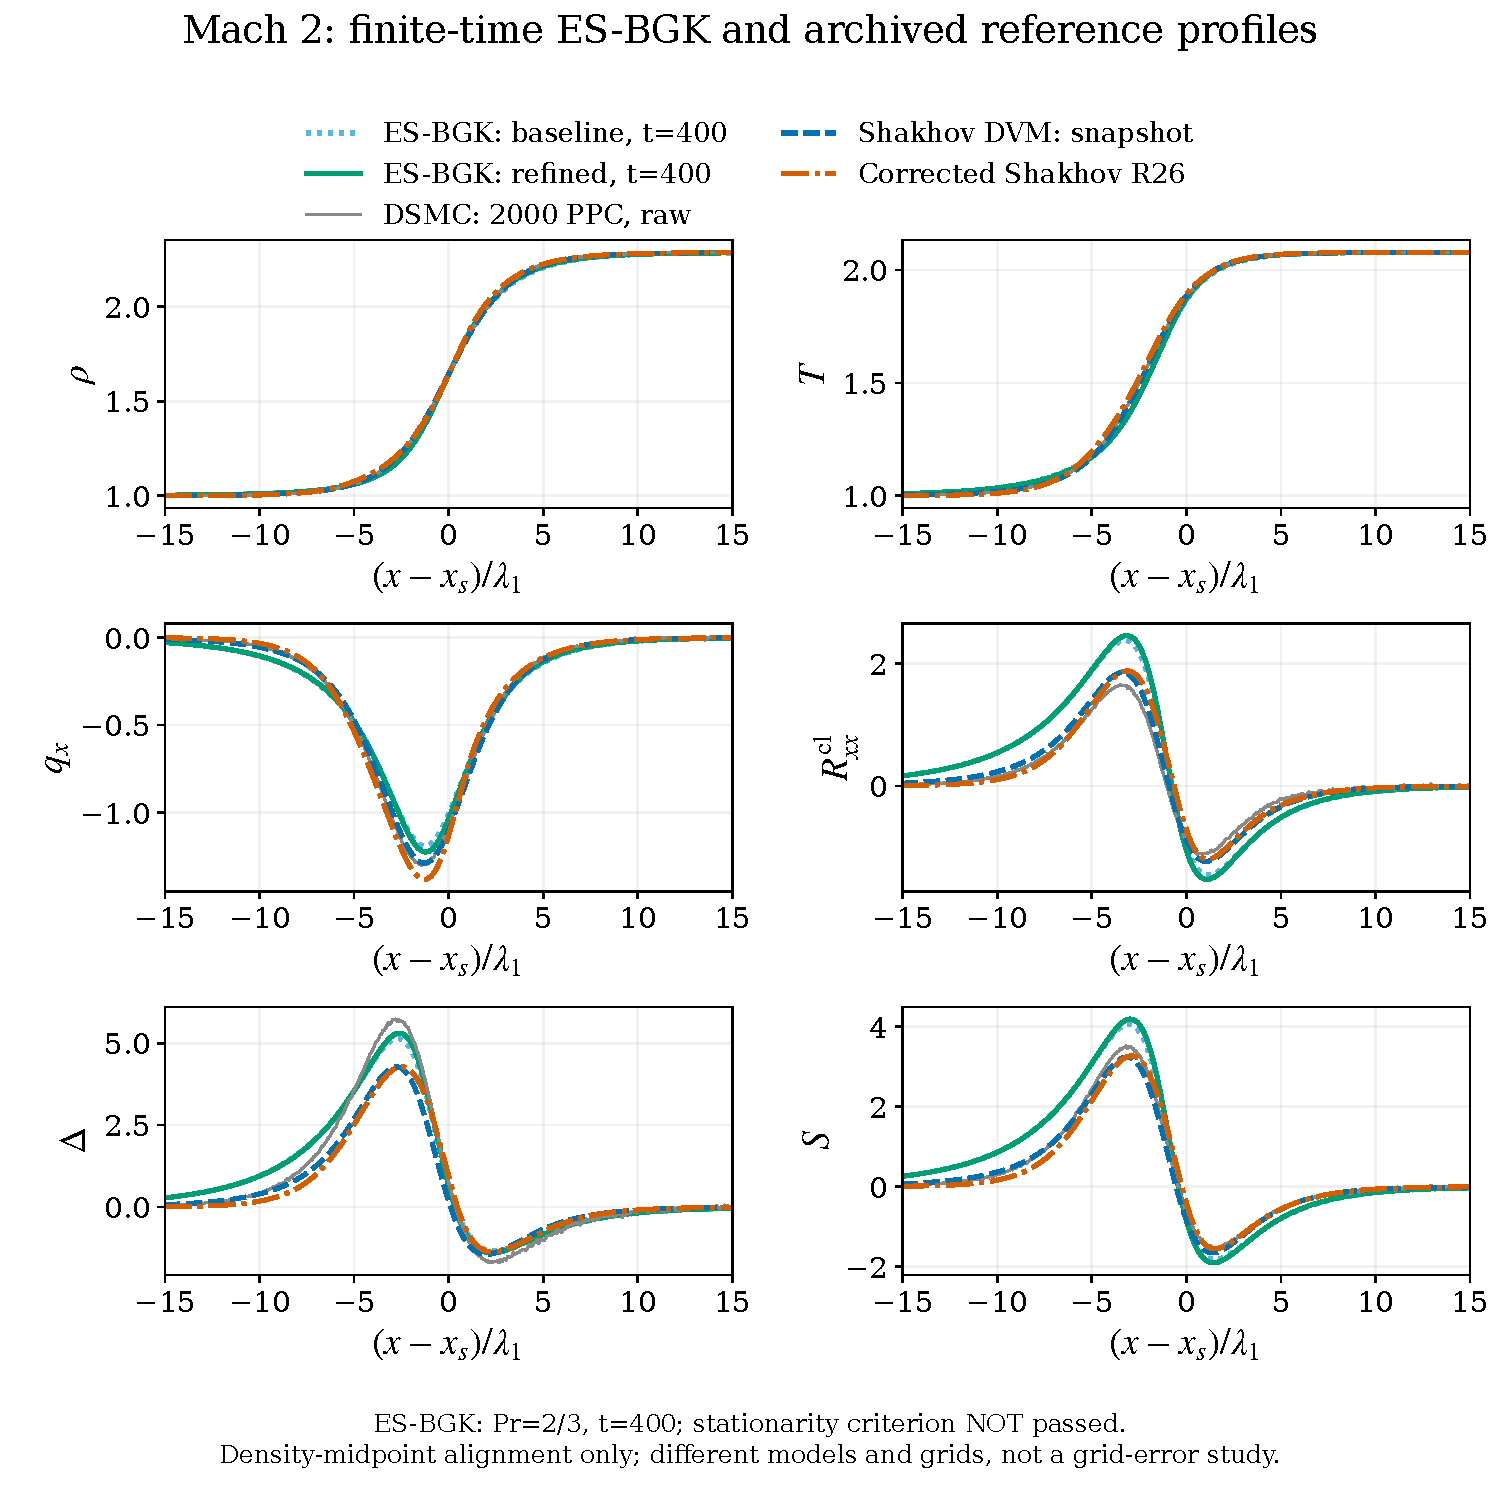
\includegraphics[width=.98\linewidth]{figures/ESBGK_M2_comparison.pdf}
\caption{Mach-2 finite-time ES-BGK profiles ($Pr=2/3$, $\mu=T$, $t\simeq400$) compared with archived 2000-PPC DSMC, Shakhov DVM and corrected Shakhov R26 profiles. The ES baseline uses $N_x=320$, $N_v=401$; the refined curve uses $N_x=640$, $N_v=801$. Only density-midpoint translations are applied; raw DSMC profiles are not smoothed. No plotted ES-BGK case has passed the stationarity criterion. The different collision models and grids prevent interpreting curve differences as numerical error alone.}
\label{fig:esbgk_m2_evolved}
\end{figure}
\clearpage\begin{figure}[p]
\centering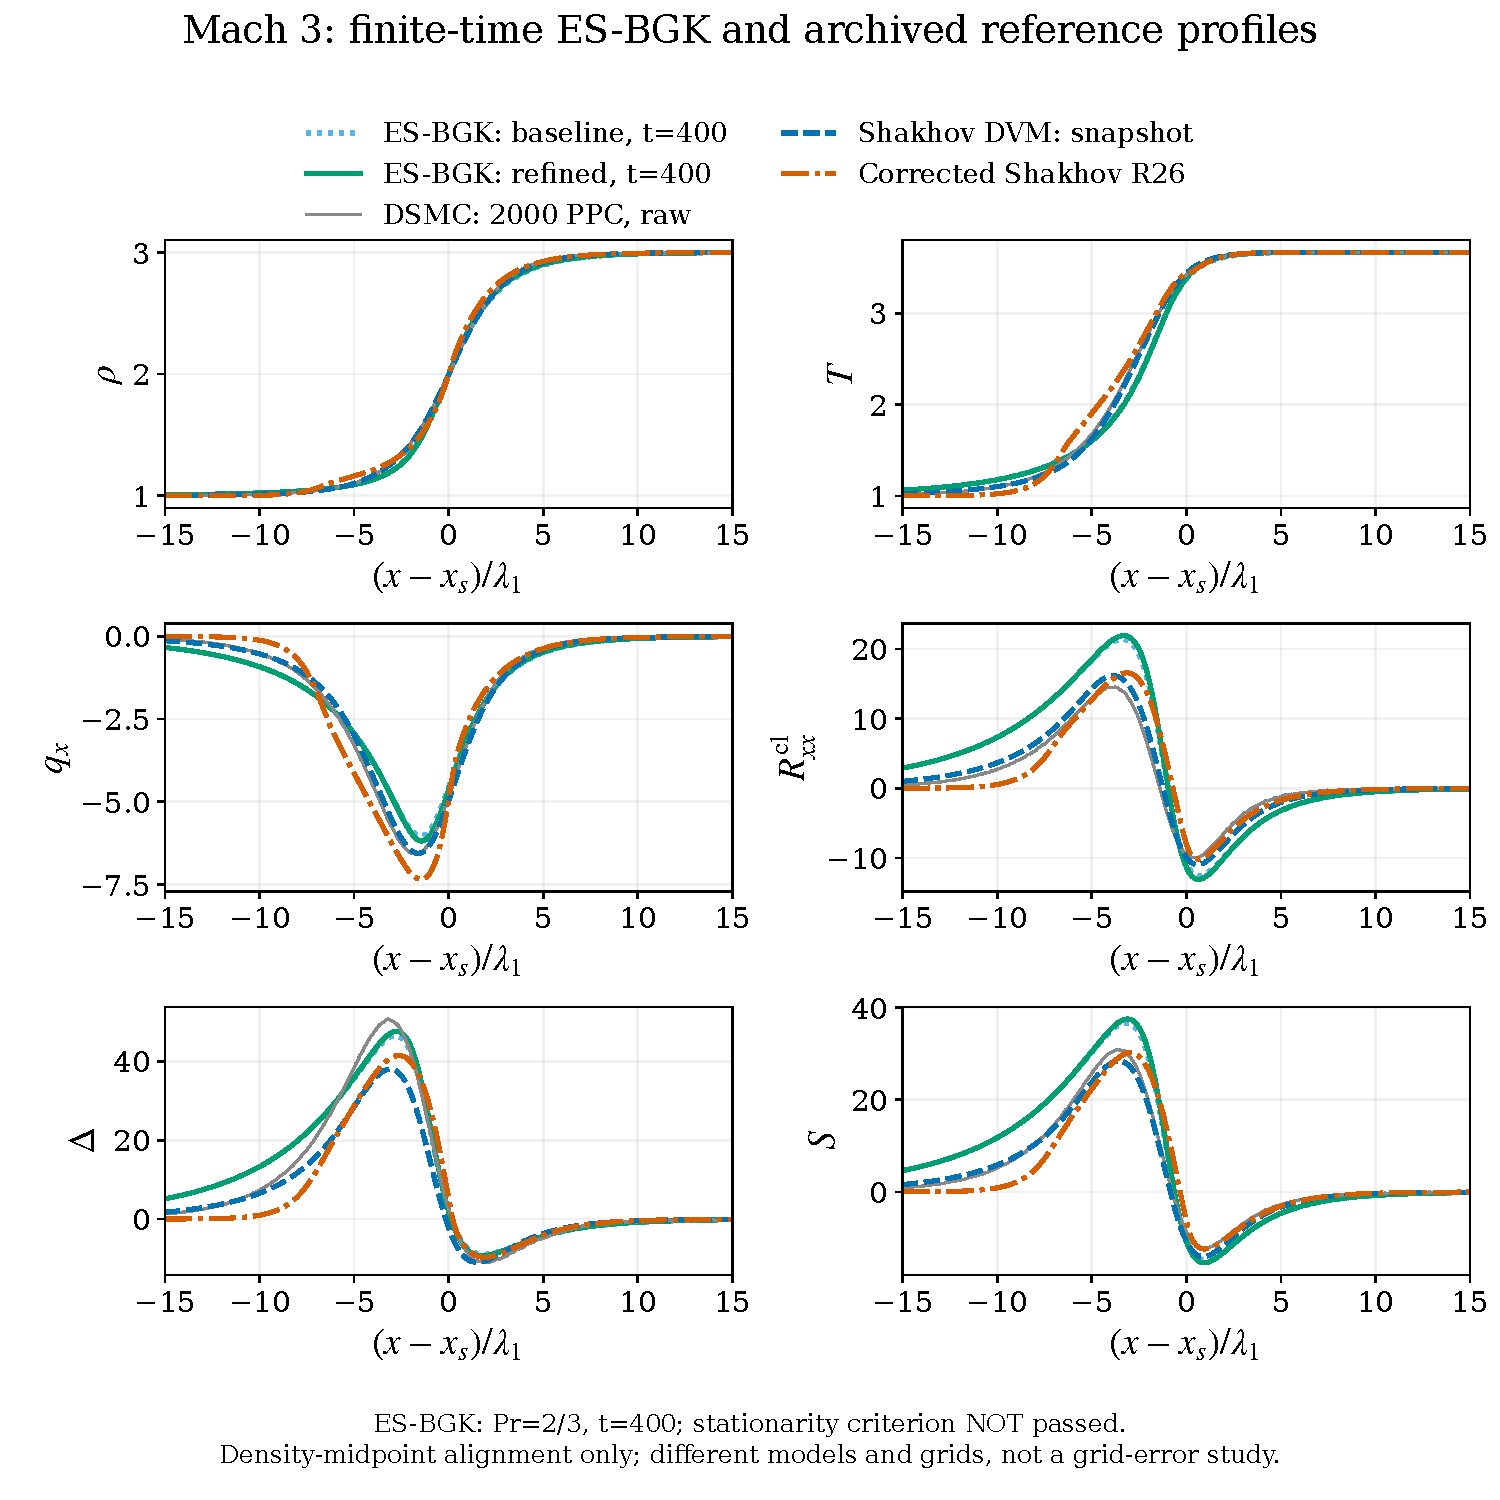
\includegraphics[width=.98\linewidth]{figures/ESBGK_M3_comparison.pdf}
\caption{Mach-3 counterpart of figure~\ref{fig:esbgk_m2_evolved}. The ES-BGK baseline uses $N_x=480$, $N_v=401$; the refined curve uses $N_x=960$, $N_v=801$. Model transport parameters, finite-time qualification and plotting conventions are the same as in figure~\ref{fig:esbgk_m2_evolved}. The archived corrected R26 profile is a separate finite-residual-qualified Shakhov calculation.}
\label{fig:esbgk_m3_evolved}
\end{figure}

\clearpage\bibliographystyle{jfm}
\bibliography{references}

\end{document}
